% Opciones empleadas:
%
% a4paper -> indica el tama? del papel, en este caso A4.
% 11pt -> tama? de la fuente 11 puntos.
% oneside -> s?o escribimos en una cara del folio.
%
% Otras opciones interesantes:
%
% twoside -> escribimos a doble cara.
% openbib -> para que las referencias bibliogr?icas tengan un salto de l?ea entre cada campo de la referencia.
%
\documentclass[a4paper,11pt,oneside]{book}

% codificaci? latin1 y s?bolos del idioma espa?l (? acentos, ...)
\usepackage[spanish]{babel}
\usepackage[utf8]{inputenc}

% puede que queramos usar el s?bolo del euro.
\usepackage{eurosym}

% El paquete fancybox nos permite crear cajas de diferentes estilos con facilidad.
% http://www.ctan.org/get/macros/latex/contrib/fancybox/fancybox.pdf
% http://www.mackichan.com/index.html?techtalk/487.htm~mainFrame
\usepackage{fancybox}
\usepackage{multicol}
\usepackage{amsmath}

% Para incluir subfiguras.
\usepackage{subcaption}

\usepackage[nottoc,numbib]{tocbibind}

% PARA incluir gr?icos en JPG => compilar con pdflatex.
\usepackage[pdftex]{graphicx}

% Para incluir gr?icos EPS => compilar con latex.
%\usepackage[dvips]{graphicx}

% Para escribir en color...
%
% ... cuando compilamos con el comando ``latex''
%\usepackage[dvips,usenames]{color}
% ... uando compilamos con el comando ``pdflatex''
 \usepackage[pdftex,usenames,dvipsnames]{color}

% Espaciado y ajuste de m?genes
\usepackage{setspace}
\onehalfspacing
% \doublespacing
\setlength{\textwidth}{15cm}
\setlength{\textheight}{22cm}

% Paquete fancyhdr -> Para modificar la cabecera y pie de p?inas.
% http://tug.ctan.org/tex-archive/macros/latex/contrib/fancyhdr/
\usepackage{fancyhdr}
\pagestyle{fancy}
\fancyhf{}
\fancyhf[HR]{\thepage}
\fancyhf[HL]{\nouppercase\rightmark}

% Package booktabs -> Para mejorar el aspecto de las tablas o cuadros.
% http://www.ctan.org/tex-archive/macros/latex/contrib/booktabs/
\usepackage{booktabs}

\usepackage{hyperref}
\hypersetup{
    colorlinks,
    linkcolor={red!50!black},
    citecolor={blue!50!black},
    urlcolor={blue!80!black}
}


% Package rotating -> Para poder girar las tablas y dibujarlas a lo largo
% del folio en vez de a lo ancho.
\usepackage{rotating}

% Packages multicol y multirow, para manejar tablas de filas y columnas m?ltiples.
\usepackage{multicol}
\usepackage{multirow}

\usepackage{color}
\usepackage{xcolor}
\usepackage{caption}
\DeclareCaptionFont{white}{\color{white}}
\DeclareCaptionFormat{listing}{\colorbox{gray}{\parbox{\textwidth}{#1#2#3}}}
\captionsetup[lstlisting]{format=listing,labelfont=white,textfont=white}

 \usepackage{listings}
 \usepackage{courier}
 \lstset{
         basicstyle=\footnotesize\ttfamily, % Standardschrift
         numberstyle=\tiny,          % Stil der Zeilennummern
         numbersep=5pt,              % Abstand der Nummern zum Text
         tabsize=2,                  % Groesse von Tabs
         extendedchars=true,         %
         breaklines=true,            % Zeilen werden Umgebrochen
         keywordstyle=\textbf,
         frame=b,
         stringstyle=\textit, % Farbe der String
         showspaces=false,           % Leerzeichen anzeigen ?
         showtabs=false,             % Tabs anzeigen ?
         xleftmargin=17pt,
         framexleftmargin=17pt,
         framexrightmargin=5pt,
         framexbottommargin=4pt,
         %backgroundcolor=\color{lightgray},
         showstringspaces=false      % Leerzeichen in Strings anzeigen ?
 }

 \lstset{literate=
  {á}{{\'a}}1 {é}{{\'e}}1 {í}{{\'i}}1 {ó}{{\'o}}1 {ú}{{\'u}}1
  {Á}{{\'A}}1 {É}{{\'E}}1 {Í}{{\'I}}1 {Ó}{{\'O}}1 {Ú}{{\'U}}1
  {à}{{\`a}}1 {è}{{\`e}}1 {ì}{{\`i}}1 {ò}{{\`o}}1 {ù}{{\`u}}1
  {À}{{\`A}}1 {È}{{\'E}}1 {Ì}{{\`I}}1 {Ò}{{\`O}}1 {Ù}{{\`U}}1
  {ä}{{\"a}}1 {ë}{{\"e}}1 {ï}{{\"i}}1 {ö}{{\"o}}1 {ü}{{\"u}}1
  {Ä}{{\"A}}1 {Ë}{{\"E}}1 {Ï}{{\"I}}1 {Ö}{{\"O}}1 {Ü}{{\"U}}1
  {â}{{\^a}}1 {ê}{{\^e}}1 {î}{{\^i}}1 {ô}{{\^o}}1 {û}{{\^u}}1
  {Â}{{\^A}}1 {Ê}{{\^E}}1 {Î}{{\^I}}1 {Ô}{{\^O}}1 {Û}{{\^U}}1
  {œ}{{\oe}}1 {Œ}{{\OE}}1 {æ}{{\ae}}1 {Æ}{{\AE}}1 {ß}{{\ss}}1
  {ç}{{\c c}}1 {Ç}{{\c C}}1 {ø}{{\o}}1 {å}{{\r a}}1 {Å}{{\r A}}1
  {€}{{\EUR}}1 {£}{{\pounds}}1
 }

 \usepackage{pgfgantt}

 \usepackage{enumitem}

% Personalizamos la separaci? entre p?rafos...
\parskip=6pt

% Personalizamos el identado en la primera l?ea del nuevo p?rafo...
\parindent=10pt

% Establecemos el n?mero m?imo de niveles de profundidad en las secciones.
\setcounter{secnumdepth}{3}

% T?ulo
\title{GNOMECAT, un editor de ficheiros GNU Gettext para o proxecto GNOME}
% Autor
\author{Marcos Chavarría Teijeiro}
% Fecha
\date{\today}


\renewcommand\lstlistingname{Fragmento de Código}
\renewcommand\lstlistlistingname{Fragmentos de Código}

\newenvironment{bottompar}{\par\vspace*{\fill}}{\clearpage}

\begin{document}

  % \maketitle sirve para generar autom?ica una portada predefinida, pero para un proyecto fin de carrera
  % de FIC no sirvir? porque no cumple las normas de presentaci?. Podemos hacer dos cosas:
  % 1. Usarla e ignorar las normas (y asumir las consecuencias que pueda tener)
  % 2. Hacernos una portada en LaTeX que cumpla las normas (menos arriesgado)
  %
        %
% Portada.
%

% Nota: Sería más cómodo emplear el comando \maketitle que genera una portada de forma automática, pero
% no incluye toda la información que es necesario incluir en la memoria de un proyecto de fin de carrera
% de la Facultad de Informática de A Coruña.
%

\begin{titlepage}

	\begin{center}

		% Logotipo de la universidad.
		
\includegraphics[width=6cm]{./eps/logo_udc.eps}
		\vspace{2cm}

		% Nombre de la facultad, de la universidad y del departamento en que se realiza el PFC.
		{\Large{\textbf{Facultade de Informática da Universidad de A Coruña}}}
		\\
		{\it \large{\textbf{Tecnoloxías da Información e das Comunicacións}}}
		\vspace{1cm}

		% Indicamos el nombre de la titulación oficial que hemos cursado con tanto esfuerzo.
		{\large PROXECTO DE FIN DE CARREIRA\\Enxeñaría Informática}
		\vspace{1cm}

		% Título
		\textbf{\Large GNOMECAT, un editor de ficheiros GNU Gettext para o proxecto GNOME}
		\vspace{7cm}
	\end{center}

	\begin{flushright}
		\begin{tabular}{ll}
			% Nombre del alumno.
			\large{\textbf{Alumno:}}	&
			\large{Marcos Chavarría Teijeiro} \\

			% Nombre del director/tutor del proyecto.
			\large{\textbf{Director:}}	&
			\large{Fernando Bellas Permuy} \\

			% Fecha.
			\large{\textbf{Fecha:}}	&
			\large{\today} \\
		\end{tabular}
	\end{flushright}

\end{titlepage}


  % FRONTMATTER: TOC, LOF, LOT y descripci?/organizaci? de la memoria.
        \frontmatter

  % Los proyectos de fin de carrera de FIC han de ir acompa?dos de una serie de documentos adicionales, algunos
  %   de ellos obligatorios (certificado, resumen, lista de palabras clave) y otros opcionales (dedicatoria
  % y agradecimientos).
  %
        \thispagestyle{empty}     % No number page, headings...
        %
% Certificado
%

\begin{center}
	\begin{minipage}[t][6cm][l]{.8\textwidth}
		\begin{center}
			% Nombre del director del proyecto
			D. {\sc Fernando Bellas Permuy}

			% A los profesores les gusta que se indique su grado o posición en la estructura de la universidad :-P
			Profesor de Escuela o Facultad Universitaria

			% Departamento al que pertenece el director y en el que se realiza el proyecto.
			Departamento de Tecnoloxías da Información e das Comunicacións

			Universidad de A Coruña
		\end{center}
	\end{minipage}
\end{center}

% El director certifica que el proyecto obra de su proyectando constituye su Proyecto de Fin de Carrera en la titulación indicada.
CERTIFICA:
Que a memoria entitulada {\it ``GNOMECAT, un editor de ficheiros GNU Gettext para o proxecto GNOME''} foi realizada por {\sc Marcos Chavarría Teijeiro} baixo a miña direción e constitúe o seu Proxecto de Fin de Carreira de Enxeñería Informática.

\vspace{5cm}

En A Coruña, a \today

% Espacio para que pueda firmar el certificado que debe acompañar al proyecto.
\vspace{3cm}

\begin{center}
	\begin{minipage}[t][4cm][l]{.5\textwidth}
	% Nombre del director del proyecto
	D. {\sc Fernando Bellas Permuy}
	\\
	Director do proxecto
	\end{minipage}
\end{center}

        \thispagestyle{empty}     % No number page, headings...

        %
% Resumen del proyecto de fin de carrera
%

\section*{Resumen:}

A internacionalización e localización de software son dous aspectos moi importantes nos que traballar en produtos software modernos. Que un programa estea localizado a un idioma que o usuario entenda é fundamental para que este usuario se sinta cómodo empregándoo.

O sistema de internacionalización e localización GNU Gettext é unha das solucións para estes dous problemas máis empregada actualmente. Para facer a localización dos programas os tradutores deben editar unha serie de ficheiros. Para facilitar dita tarefa existen ferramentas denominadas CAT (\emph{Computer Assisted Translation}).

Neste proxecto preténdese crear unha nova ferramenta para a asistencia á tradución centrada na organización de software libre GNOME. Dita ferramenta editará os ficheiros de GNU Gettext e empregará unha interface construída coas ferramentas que aporta o stack de GNOME.

Para facilitar a participación de futuros desenvolvedores empregarase unha linguaxe de programación cunha sintaxe moi amigable en contraste coa empregada noutros proxectos de GNOME. En concreto empregarase a linguaxe de programación Vala.

Este proxecto foi elaborado durante dous veráns consecutivos como parte do programa Google Summer of Code.

        \thispagestyle{empty}     % No number page, headings...

        %
% Palabras clave
%

\section*{Lista de palabras clave:}

\begin{itemize}
  \item GNOME
  \item Localización (L10N)
  \item Internacionalización (I18N)
  \item Computer Assisted Translation (CAT)
  \item GTK+
  \item Vala
  \item GNU Gettext
  \item Google Summer of Code
\end{itemize}

        \thispagestyle{empty}     % No number page, headings...

        %
% Agradecimientos
%

\section*{Agradecementos}

Quero aproveitar este espazo para amosar o meu agradecemento a todas aquelas persoas que dunha maneira ou outra estiveron relacionadas coa elaboración deste proxecto. Gustaríame agradecer a axuda prestada polos mentores dos dous Summer of Code que fixen e a guía que me ofreceu Fernando Bellas para poder presentar a realización deste programa como o meu Proxecto de Fin de Carreira. Quero, ademais, facer facer unha especial mención a Daniel Mustieles, coordinador do equipo de tradutores de GNOME ao castelán, pai deste proxecto e a persoa que máis me axudou para realizalo. Tamén, expresar o meu agradecemento a todos os usuarios e desenvolvedores de GNOME que dende un chat de IRC, un correo ou un comentario dun blogue me axudaron a mellorar o programa.

Gustaríame agradecer tamén as horas de dedicación de todo o persoal docente que dende os tres anos cos que empecei a ir a escola, ata as últimas materias da carreira me estiveron formando. Sen todo o tempo que dedicaron a formarme non tería os coñecementos necesarios sobre a informática e sobre a vida para poder levar a cabo o presente proxecto.

Non me quero esquecer de todas o resto de persoas que me acompañan neste camiño que é a vida. Quero dar grazas a meus pais, tíos, avós  e o resto da miña familia que sempre me apoiou canto puido e máis.

Teño a sorte de contar con moitos e bos amigos e amigas así que por último e non por elo menos importante gustaríame darlles a todos eles as grazas por eses anacos de tempo agora xa inmortais nos que xunto a eles tiven a oportunidade de viaxar, saltar, bailar, estudar, rir, chorar, falar, cantar, berrar, comer, soñar, beber... en definitiva, de vivir. 

A todos vós, moitas grazas!


\begin{flushright}
  Marcos Chavarría Teijeiro \\
  A Coruña, 15 de xuño de 2015
\end{flushright}


        \thispagestyle{empty}     % No number page, headings...

        
\begin{bottompar}
\begin{center}


\includegraphics{img/cclicence.png}

\textbf{Este traballo está licenciado baixo Creative Commons Attribution-ShareAlike 4.0 International License.}
\end{center}
\end{bottompar}
        \thispagestyle{empty}     % No number page, headings...


        \tableofcontents
        \listoffigures
        %\listoftables


  % MAINMATTER: El contenido, cap?ulo a cap?ulo, de la memoria del PFC.
        \mainmatter
        %
% Frontmatter - Introducción. Los miembros del tribunal que juzgan los PFC's tienen muchas más memorias que leer, por lo que
%	agradecerán cualquier detalle que permita facilitarles la vida. En este sentido, realizar una pequeña introducción,
%	comentar la organización y estructura de la memoria y resumir brevemente cada capítulo puede ser una buena práctica
%	que permita al lector centrarse fácilmente en la parte que más le interesa.
%

\chapter[Introdución]{Introdución}

Neste capítulo de introdución intentarase explicar os aspectos necesarios para entender en que consiste o proxecto, o que me fixo levalo a cabo e, por último, unha explicación da estrutura da presente memoria.

\section{Internacionalización e Localización de Software}
A internacionalización é o proceso de adaptación dun software para que este poida ser traducido a varios idiomas e ser usado en diferentes rexións sen modificar a súa enxeñería. A localización de software consiste na adaptación de dito software a unha rexión determinada. Isto, aínda que afecta fundamentalmente ó idioma, tamén ten outros elementos como as divisas, a forma de formatar as datas ou a utilización de determinados símbolos que nunhas áreas teñen un significado e noutras outro distinto.

Trátase dun aspecto moi importante do mundo do software pois se ben unha persoa que saiba inglés (o idioma orixe da maior parte dos programas) a internacionalización dos programas é un problema de comodidade, para o que non entenda a lingua de Shakespeare; trátase dun problema de usabilidade. Unha persoa que non sexa nativa dixital e que non entenda inglés terá serios problemas para entender calquera software moderno non localizado.

\section{O Proxecto GNOME}
GNOME é ambiente de escritorio, unha infraestrutura de desenvolvemento e unha comunidade de software libre.

Como ambiente de escritorio foi creado polos mexicanos Miguel de Icaza e Federico Mena en 1997 como alternativa a KDE compatible coa licencias GPL\footnote{En aquel momento KDE empregaba unha licencia QPL que aínda que era libre non era compatible GPL.}. Trátase de crear un solución software para todo o mundo poñendo interese en aspectos como a accesibilidade, a internacionalización ou a usabilidade.

Como infraestrutura de desenvolvemento GNOME prové unha gran cantidade de aplicativos e bibliotecas para crear os programas tanto para a plataforma GNOME como para outras plataformas.

\begin{figure}[h!]
    \centering
    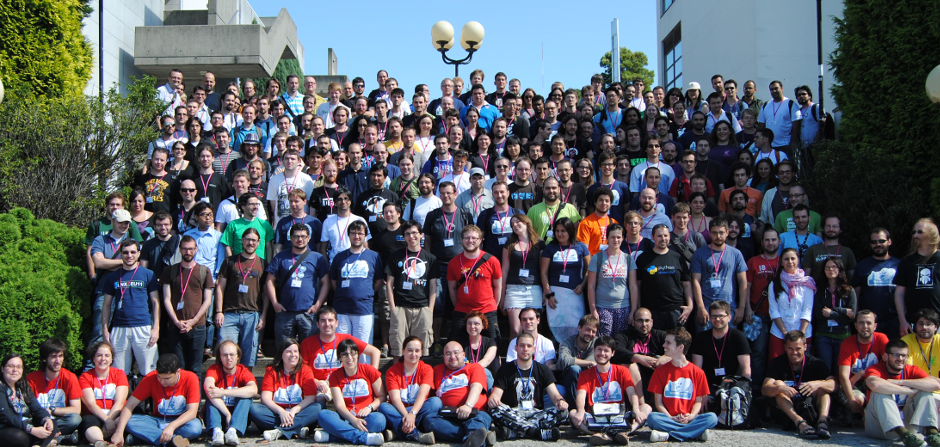
\includegraphics[width=\textwidth]{img/guadec_2012.png}
    \caption{GUADEC A Coruña 2012}
    \label{fig:guadec2012}
\end{figure}

Como comunidade reúne a gran cantidade de persoas, tanto voluntarias como profesionais, que axudaron e axudan a que o proxecto siga adiante. Dentro desta comunidade poden encontrarse persoas de moi diversa procedencia e oficio sendo a maioría programadores, aínda que tamén existen persoas dedicadas a marketing, á administración, ó deseño ou á administración de sistemas, entre outras.

GNOME ademais pon especial interese en intentar sumar xente ao proxecto. Participa sempre no programa de iniciación ao desenvolvemento de software libre Summer of Code promovido por Google e é promotor da iniciativa Outreachy\footnote{Inicialmente denominábase GNOME Outreach Program for Women} que pretende acercar ás mulleres á contribución en software libre.

En Europa a comunidade de GNOME reúnese na GUADEC, que é o acrónimo de \textbf{G}NOME \textbf{U}sers \textbf{A}nd \textbf{D}evelopers \textbf{C}onference. Un evento que se fai anualmente e que no ano 2012 tivo lugar na Facultade de Informática da Coruña~(Figura~\ref{fig:guadec2012}).

\subsection{Localización e Internacionalización no Proxecto GNOME}
Como xa dixemos un dos aspectos máis importante para o proxecto GNOME é o acercamento ás persoas e para lograr isto ponse pleno interese na internacionalización e na localización do ambiente de escritorio e das aplicacións de GNOME. GNOME está traducido a máis de 50 idiomas moitos dos cales teñen máis do 90\% das cadeas traducidas.

O proxecto GNOME emprega o sistema GNU Gettext para internacionalizar e localizar os seus programas e conta con unha plataforma web de nome Damned Lies para xestionar a localización de todo o proxecto. Este programa amosa as estatísticas do estado actual das traducións e axuda a xestionar o ciclo de traballo dos tradutores. Permite asignar módulos a tradutores, que os tradutores suban os ficheiros traducidos e que se faga unha revisión do traballo do tradutor.

Outros proxectos de software como Facebook, Twitter ou, dentro do software libre, Ubuntu e Fedora contan con plataformas online dende as que se pode facer directamente a tradución. GNOME opta por facer a tradución \emph{offline} para que esta sexa dunha maior calidade.

Para que os tradutores poidan traballar de forma cómoda é necesario a existencia de ferramentas que lle faciliten o traballo. Estas ferramentas coñécense como CAT, que é o acrónimo de Computer Assisted Translation. Neste traballo preténdese realizar unha destas ferramentas centrada no proxecto GNOME.

\section{Google Summer of Code}
O Summer of Code (xeralmente abreviado SoC ou GSoC) é un programa da empresa estadounidense Google para o fomento do desenvolvemento de software libre entre estudantes de todo o mundo. Realizase unha vez ao ano durante o verán e os participantes deberán ser estudantes, maiores de 18 anos e non ter durante ese verán ningún traballo remunerado.

Existen diversas organizacións de software libre que se presentan para participar no programa aportando unha lista de ideas sobre a que os futuribles participantes deberán presentar un proxecto do que queren traballar durante o verán. Se os estudantes son elixidos, a organización asignará a cada estudante un ou máis mentores que deberán guiar ao participante a levar a cabo as tarefas asignadas. Existen avaliacións tanto para os estudantes como para os mentores. Se o estudante é avaliado con éxito recibirá 5500 dólares polo traballo realizado.

Trátase dun programa de moito éxito en todo o mundo e sobre todo en países como India, onde carecen de iniciativas locais similares. Na edición do verán do ano 2014, participaron 190 organizacións entre as cales se atopan principales axentes no mundo do software libre como GNOME, KDE, GNU ou Firefox e 1307 estudantes de todo o mundo.

\section{Motivación}
Durante a GUADEC Hispana\footnote{A GUADEC Hispana é a versión para hispanofalantes da GUADEC} 2012 que tivo lugar en A Coruña dentro da GUADEC do mesmo ano, asistín a unha charla impartida por Daniel Mustieles, o coordinador do equipo de tradutores ao castelán do proxecto GNOME. Nesta charla Daniel, resaltaba a necesidade de que o programa actual de asistencia á tradución fose mellorado.

GTranslator está escrito en C e emprega unha biblioteca chamada GObject para facer orientación a obxectos dentro de C. Isto fai que achegarse ó proxecto sexa complicado para un novato polo que falando con outros desenvolvedores da plataforma decidiuse que era mellor reescribir o programa noutra linguaxe e ao mesmo tempo arranxar algúns erros que tiña anteriormente o programa.

Durante o ano seguinte presentei un proxecto para o Google Summer of Code para escribir un novo programa CAT para a plataforma GNOME. Este programa sería unha re-escritura e re-deseño de GTranslator nunha linguaxe de programación moito máis amigable, Vala.

\section{Estrutura da memoria}

A memoria componse de oito capítulos nos que se expón os pasos que se deron para crear o programa GNOMECAT.

\paragraph*{Capítulo 1. Introdución.}
Este capítulo. Nel intentamos explicar de forma resumida en que consiste este proxecto, as motivacións para levalo a cabo e a estrutura da memoria.

\paragraph*{Capítulo 2. Estado do Arte.}
Explicaranse as tecnoloxías empregadas no ámbito da internacionalización e localización de software en xeral e software libre en particular. Farase ademais unha análise de diversas ferramentas do mercado.

\paragraph*{Capítulo 3. Fundamentos Tecnolóxicos.}
Enumeraranse as ferramentas e bibliotecas empregadas durante a elaboración deste proxecto.

\paragraph*{Capítulo 4. Metodoloxía.}
Detallarase o conxunto de prácticas e métodos seguidos durante a realización do programa e que están inspiradas fundamentalmente na metodoloxía eXtreme Programming.
\paragraph*{Capítulo 5. Planificación e Seguimento.}
Explicarase a planificación e o seguimento de cada unha das iteracións que fixemos para elaborar o programa.

\paragraph*{Capítulo 6. Análise de Requisitos.}
Explicarase como se levou a cabo o análise de requisitos para esta aplicación e detallarase cada un dos mesmos.

\paragraph*{Capítulo 7. Deseño e implementación.}
Neste capítulo explicaremos detalles concretos do deseño e a implementación de certas partes do programa.

\paragraph*{Capítulo 8. Conclusións e Traballo Futuro.}
Relataranse as conclusións despois da elaboración do presente proxecto e explicaranse posibles liñas de traballo futuro.






        \chapter{Estado do Arte}

Neste capítulo explicarase como funciona a internacionalización e localización con GNU Gettext. Ademais analizaremos as diferentes alternativas que existen no mercado como ferramentas de asistencia á tradución e ás características que cada unha incorpora. Ó final faremos un resumo das características que empregan os programas CAT\footnote{Computer Assisted Translation}.

\section{Internacionalización e localización con GNU Gettext}
Gettext é un sistema para a internacionalización e localización amplamente usado en entornos UNIX. Conta con varías implementacións, sendo a primeira de Sun Microsystems no ano 1990. A implementación máis usada é a que GNU liberou no ano 1995. Pese ser unha solución antiga, é a día de hoxe a mellor que se pode atopar no mercado.

Para internacionalizar un programa con GNU Gettext non empregaremos as cadeas de texto directamente como podería ser no Fragmento de Código~\ref{code-no-i18n}.

\begin{lstlisting}[language=C,label=code-no-i18n,caption=helloworld.c (Sen Internacionalizar)]
#include <stdio.h>

int
main ()
{
    printf ("Hello World!");
}
\end{lstlisting}

En lugar diso chamaremos a unha función especial que proporciona Gettext de nome \lstinline{gettext()} pero que é máis empregada a través do seu alias \lstinline{_()}. Ademais configuraremos o programa para que colla a tradución do idioma que queiramos. Desta forma o programa anterior quedaría como se pode ver no Fragmento de Código~\ref{code-i18n}.

\begin{lstlisting}[language=C,label=code-i18n,caption=helloworld.c]
#include <stdio.h>
#include <locale.h>
#include <libintl.h>

#define _(str) gettext(str)

#define

int
main ()
{
    setlocale (LC_ALL, "");
    bindtextdomain ("helloworld", "/usr/local/share/locale");
    textdomain ("helloworld");

    printf (_("Hello World!"));
}
\end{lstlisting}

A función \lstinline{gettext()} é a encargada de substituír a cadea orixinal pola tradución. Non obstante, vemos que debemos configurar algunhas cousas antes de poder chamar á función.

En primeiro lugar debemos establecer a linguaxe que queremos empregar no programa. Para iso usamos a función \lstinline{setlocale()}. O primeiro argumento da función determina que parte do locale actual queremos modificar. Entre outras podemos atopar:

\begin{itemize}
    \item \textbf{LC\_ALL.} Queremos cambiar todo.
    \item \textbf{LC\_ADDRESS.} Queremos cambiar a forma de formatar os enderezos.
    \item \textbf{LC\_MESSAGES.} Os mensaxes do programa.
    \item \textbf{LC\_NUMERIC.} O formatado das cantidades non monetarias
    \item \textbf{LC\_TIME.} O formatado de datas e horas.
\end{itemize}

Por último especificamos o código de idioma ou no caso de empregar a cadea baleira empregamos os valores das variables de entorno.

Os códigos de idioma empregan a normativa ISO 639 polo que son da forma $$language[\_territory][.codeset][@modifier]$$ Por exemplo o código do galego empregando codificación UTF-8 é \lstinline{gl\_ES.UTF-8}.

Ademais debemos indicarlle ó programa onde ten que atopar as traducións. Para iso empregamos a función \lstinline{bindtextdomain()} que liga un nome de dominio a unha ruta dentro do sistema e a función \lstinline{textdomain()} que lle indica o programa cal é o nome de dominio que debe empregar. Un dominio é un conxunto de cadeas que se empregan nunha parte determinada dun programa. Cada dominio debe ter un nome de dominio único dentro dun programa.

Con estes parámetros Gettext xa é capaz de atopar as traducións que no caso do programa anterior atoparíanse en \emph{/usr/local/share/locale/gl/LC\_MESSAGES/helloworld.mo}.

Unha vez que internacionalizamos o nosos programa debemos traducir as cadeas. Pero para traducir as cadeas debemos extraelas antes do código fonte. Para iso empregaremos a utilidade \emph{xgettext}. Empregando as opcións adecuadas obtemos no ficheiro que se amosa no Fragmento de Código~\ref{potfile}.

\begin{lstlisting}[label=potfile,caption=helloworld.pot]
# SOME DESCRIPTIVE TITLE.
# Copyright (C) YEAR THE PACKAGE'S COPYRIGHT HOLDER
# This file is distributed under the same license as the PACKAGE package.
# FIRST AUTHOR <EMAIL@ADDRESS>, YEAR.
#
#, fuzzy
msgid ""
msgstr ""
"Project-Id-Version: PACKAGE VERSION\n"
"Report-Msgid-Bugs-To: \n"
"POT-Creation-Date: 2014-11-12 19:24+0100\n"
"PO-Revision-Date: YEAR-MO-DA HO:MI+ZONE\n"
"Last-Translator: FULL NAME <EMAIL@ADDRESS>\n"
"Language-Team: LANGUAGE <LL@li.org>\n"
"Language: \n"
"MIME-Version: 1.0\n"
"Content-Type: text/plain; charset=CHARSET\n"
"Content-Transfer-Encoding: 8bit\n"

#: helloworld.c:14
#, c-format
msgid "Hello World!"
msgstr ""
\end{lstlisting}

Os ficheiros Gettext coa estensión \emph{POT} trátanse de plantillas xenéricas para todos os idiomas. Para obter o arquivo especifico para o noso idioma debemos empregar a ferramenta \emph{msginit} coa que obteremos un ficheiro como o que se pode ver no Fragmento de Código~\ref{untrans-pofile}.

\begin{lstlisting}[label=untrans-pofile,caption=helloworld.po (Sen Traducir)]
# Galician translations for HELLOWORLD package.
# Copyright (C) 2014 THE HELLOWORLD COPYRIGHT HOLDER
# This file is distributed under the same license as the ch package.
# Marcos Chavarría Teijeiro <chavarria1991@gmail.com>, 2014.
#
msgid ""
msgstr ""
"Project-Id-Version: ch 01\n"
"Report-Msgid-Bugs-To: \n"
"POT-Creation-Date: 2014-11-12 19:24+0100\n"
"PO-Revision-Date: 2014-11-12 19:54+0100\n"
"Last-Translator: Marcos Chavarría Teijeiro <chavarria1991@gmail.com>\n"
"Language-Team: Galician\n"
"Language: gl_ES\n"
"MIME-Version: 1.0\n"
"Content-Type: text/plain; charset=ISO-8859-1\n"
"Content-Transfer-Encoding: 8bit\n"

#: helloworld.c:14
#, c-format
msgid "Hello World!"
msgstr ""
\end{lstlisting}

Desta forma obtemos un ficheiro Gettext PO que é o ficheiro que temos que editar. Traducindo o arquivo obtemos algo como o Fragmento de Código~\ref{trans-pofile}.

\begin{lstlisting}[label=trans-pofile,caption=helloworld.po (Traducido)]
# Galician translations for HELLOWORLD package.
# Copyright (C) 2014 THE HELLOWORLD COPYRIGHT HOLDER
# This file is distributed under the same license as the HELLOWORLD package.
# Marcos Chavarría Teijeiro <chavarria1991@gmail.com>, 2014.
#
msgid ""
msgstr ""
"Project-Id-Version: HELLOWORLD 1.0\n"
"Report-Msgid-Bugs-To: \n"
"POT-Creation-Date: 2014-11-12 19:24+0100\n"
"PO-Revision-Date: 2014-11-12 19:54+0100\n"
"Last-Translator: Marcos Chavarría Teijeiro <chavarria1991@gmail.com>\n"
"Language-Team: Galician\n"
"Language: gl_ES\n"
"MIME-Version: 1.0\n"
"Content-Type: text/plain; charset=ISO-8859-1\n"
"Content-Transfer-Encoding: 8bit\n"

#: helloworld.c:14
#, c-format
msgid "Hello World!"
msgstr "Ola Mundo!"
\end{lstlisting}

Antes de poder empregar o ficheiro no noso programa temos que compilalo. Para iso empregamos a utilidade msgfmt coa que obtemos o ficheiro helloworld.mo. Se movemos o ficheiro o directorio adecuado (o que especificamos en \lstinline{textdomain()}) o noso programa xa estará localizado.

\subsection{Ficheiros Gettext PO}
Como xa dixemos antes, os ficheiros PO son os ficheiros que temos que editar para localizar o noso programa. Primeiro dicir que se trata ficheiros de texto plano e que polo tanto podemos editar con calquera editor de ficheiros de texto plano. Non obstante, o ideal é empregar algunha ferramenta que nos facilite a tarefa como pode ser unha ferramenta CAT.

As súas principais características son:

\paragraph{Soporte de plurais}
Algo que pode parecer trivial como o soporte de plurais deixa de selo cando consideramos que non todos as linguaxes do mundo empregan dous plurais. A lingua eslovaca, por exemplo, conta con tres formas de plural de forma que o plural faise diferente para 1, 3 e 5 elementos.

Gettext representa a forma de plural de cada linguaxe con unha cadea da seguinte forma: $$nplurals=n; plural=exp;$$ Onde $n$ representa o número de plurais da linguaxe e $exp$ a expresión para calcular cando debemos empregar cada forma. Por exemplo a forma plural do galego representase como $nplurals=2; plural=(n != 1);$. Isto é que temos 2 plurais e que so se emprega a forma singular cando o número de elementos é igual a $1$.

No código fonte para que GetText escolla a tradución adecuada temos que empregar a función \lstinline{ngettext}. Esta función recibe como parámetros a cadea orixinal en singular, a cadea orixinal en plural e o número de elementos. No Fragmento de Código~\ref{plural-code} temos un exemplo:

\begin{lstlisting}[label=plural-code,language=C,caption=Plurais en GetText (Código Fonte).]
[...]
    printf (ngettext ("We have %d car.", "We have %d cars.", n), n);
[...]
\end{lstlisting}

A cadea do ficheiro PO (Fragmento de Código~\ref{plural-pofile}) correspondente ó código anterior pódese ver no seguinte fragmento de código. Vemos como temos unha entrada \lstinline{msgstr} por cada plural. Desta forma o plural número $0$ corresponde ós singular e o plural número $1$ correspondese coa primeira forma do plural.

\begin{lstlisting}[label=plural-pofile,caption=Plurais en GetText (Ficheiro PO).]
#: helloworld.c:19
#, c-format
msgid "We have %d car."
msgid_plural "We have %d cars."
msgstr[0] "Temos %d coche."
msgstr[1] "Temos %d coches."
\end{lstlisting}


\paragraph {Marcado de traducións difusas}
Permítese marcar certas traducións como difusas de forma que o tradutor indica que non estar seguro de que dita tradución sexa correcta. Se marcásemos a tradución \emph{"Hello World!"} como difusa o ficheiro PO tería o aspecto que se pode ver no Fragmento de Código~\ref{fuzzy-po-file}.

\begin{lstlisting}[label=fuzzy-po-file,caption=Ficheiro POT con comentario.]
[...]
#: helloworld.c:15
#, c-format
#, fuzzy
msgid "Hello World!"
msgstr ""
[...]
\end{lstlisting}

\paragraph {Formato das traducións}
Os ficheiro PO permite indicar se as cadeas a traducir teñen un formato determinado. Por exemplo, a cadea do exemplo no Fragmento de Código~\ref{trans-pofile} pódese ver que ten o flag \lstinline{c-format} debido a que é parte dunha sentencia printf e podería levar indicadores de formato da forma \lstinline{%s}.

\paragraph {Cabeceira con metadatos}
Existe unha cadea especial nos documentos Gettext PO. Trátase da cadea baleira que serve para almacenar metadatos do ficheiro. No fragmento de código \ref{trans-pofile} podemos ver istos metadatos. Algúns dos metadatos existentes son:

\begin{itemize}
    \item \textbf{Project-Id-Version.} Nome único para o proxecto deste arquivo de tradución.
    \item \textbf{Report-Msgid-Bugs-To.} Ligazón onde reportar errores nas cadeas orixinais ou para pedir contexto para facer a tradución.
    \item \textbf{POT-Creation-Date.} Data de creación do ficheiro POT.
    \item \textbf{PO-Revision-Date.} Data da última actualización das traducións.
    \item \textbf{Last-Translator.} Nome e enderezo de correo electronico do último traductor.
    \item \textbf{Language-Team.} Enderezo de correo eléctronico do equipo de traductores.
    \item \textbf{Language.} Linguaxe do ficheiro expresada coa codificación ISO 639.
    \item \textbf{Content-Type.} Tipo MIME do ficheiro, que será sempre \lstinline{text/plain} e codificación dos caracteres.
    \item \textbf{Plural-Forms.} Expresión da forma plural empregada.
\end{itemize}

Ademais destes campos, nos comentarios, gárdanse os nomes de todas as persoas que contribuíron a esta tradución.

\paragraph{Gardado dos orixes das cadeas}
Gettext almacena para cada cadea en que lugares do código aparece esta. O cal pode ser moi interesante para implentar a previsualización das traducións. Por exemplo no Fragmento de Código~\ref{trans-pofile} vemos como a cadea \emph{"Hello World!"} pode atoparse na liña 14 do ficheiro \lstinline{helloworld.c}.

\paragraph{Comentarios dos programadores}
É unha función moi importante xa que en moitas ocasións nas linguaxes a mesma palabra empregase como verbo ou como nome polo que en ocasións é importante incorporar un contexto para esa tradución. Para facer isto é necesario simplemente poñer un comentario no programa antes de empregar a cadea. Por exemplo no Fragmento de Código~\ref{prog-comment-code}, estamos engadindo un comentario a cadea \emph{"Hello World!"}.

\begin{lstlisting}[label=prog-comment-code,language=C,caption=Tradución con comentario.]
[...]
    // Translators: We are just waving the world.
    printf (_("Hello World!"));
[...]
\end{lstlisting}

O ficheiro POT resultado tería a forma que se pode ver no Fragmento de Código~\ref{prog-comment-pofile}.

\begin{lstlisting}[label=prog-comment-pofile,caption=Ficheiro POT con comentario.]
[...]
#. Translators: We are just waving the world.
#: helloworld.c:15
#, c-format
msgid "Hello World!"
msgstr ""
[...]
\end{lstlisting}


\paragraph{Comentarios dos tradutores}
A biblioteca permite que os tradutores comenten as cadeas. No Fragmento de Código~\ref{trans-comment-pofile} podemos ver o aspecto que tería o ficheiro PO se engadimos un comentario á cadea \emph{"Hello World!"}.

\begin{lstlisting}[label=trans-comment-pofile,caption=Ficheiro PO con comentario.]
[...]
# This is a note from translators.
#: helloworld.c:15
#, c-format
msgid "Hello World!"
msgstr ""
[...]
\end{lstlisting}

\section{Ferramentas CAT do mercado}
\label{sec:ferramentascat}
Nesta sección analizaremos algunhas das ferramentas de asistencia á tradución existentes. Veremos as características que incorporan estes programas así como estudar a súa interface de usuario.

\subsection{GTranslator}
GTranslator é a aplicación oficial do proxecto GNOME para a asistencia á tradución. Este aplicativo só permite a tradución de arquivos GNU Gettext. As característica máis destacables deste programa son a posibilidade de abrir varios ficheiros en diferentes lapelas, soporte de memorias de tradución, perfiles para diferentes tradutores, edición dos comentarios dos ficheiros .po e un sistema de plugins que permite estender a ferramenta.

\begin{figure}[h]
    \centering
    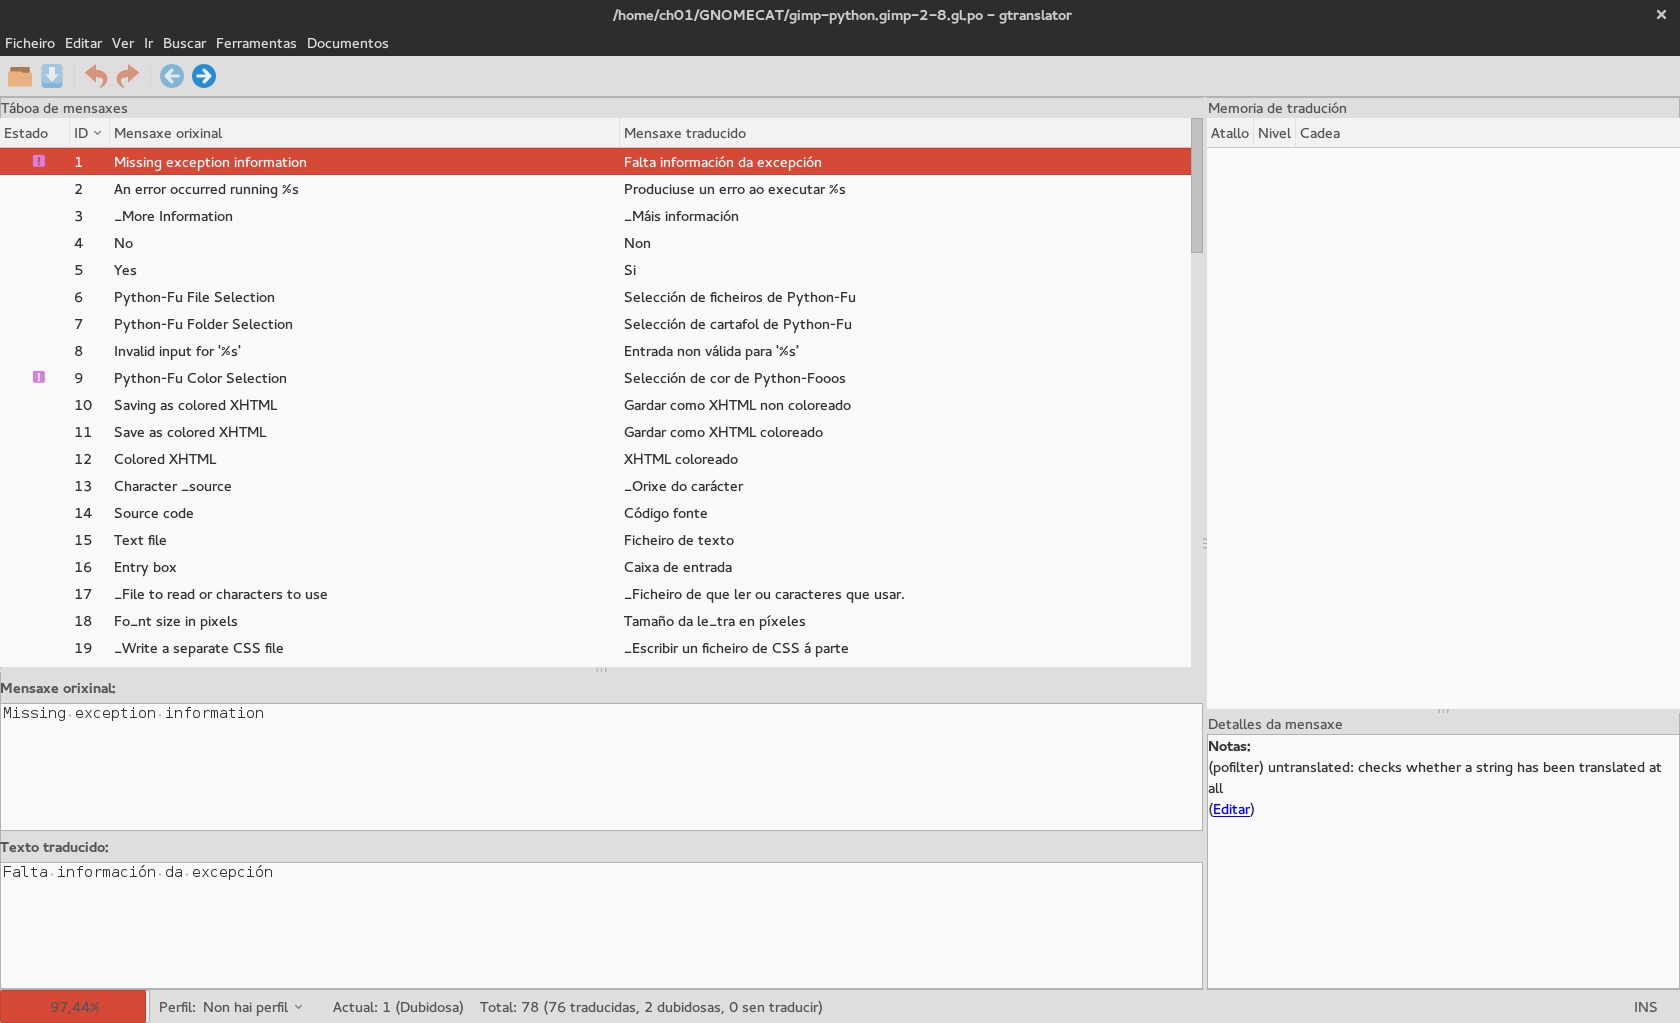
\includegraphics[width=\textwidth]{img/captura_gtranslator.png}
    \caption[Interface de GTranslator]{Interface de GTranslator}
    \label{fig:gtranslator}
\end{figure}

En canto a interface, como podemos ver na Figura~\ref{fig:gtranslator}, a parte máis importante do programa é a a lista de mensaxes. Abaixo desta lista temos un panel onde se pode editar cada mensaxe e á súa dereita a memoria de tradución. A disposición dos elementos desta interface é configurable xa que permite mover e ampliar cada un dos módulos. O programa tamén incorpora atallos de teclado que permiten moverse polo documento e seleccionar cada elemento da memoria de tradución.

Este programa pese a ser o aplicativo oficial de GNOME é moi pouco usado. As razóns disto son a ausencia dunha característica chave que o diferencie doutras ferramentas do mercado, a presenza de fallas importantes que afectan a usabilidade e a ausencia dun mantedor que resolva estes problemas.

\subsection{Lokalize}
Lokalize é o programa oficial para o soporte á tradución en KDE. Foi escrita dende cero empregando a tecnoloxía de KDE Platform 4 e baseándose no código de KBabel. As súas características máis destacables son: o soporte para ficheros GNU Gettext e o formato QT TS, entre outros; a xestión de proxectos incorporando unha vista que permite ver un resumo de cada ficheiro dentro do proxecto; uso de memorias de tradución e de glosarios; comprobación da ortografía e vista previa das traducións a partir de scripts feitos polo usuario.

\begin{figure}[h]
    \centering
    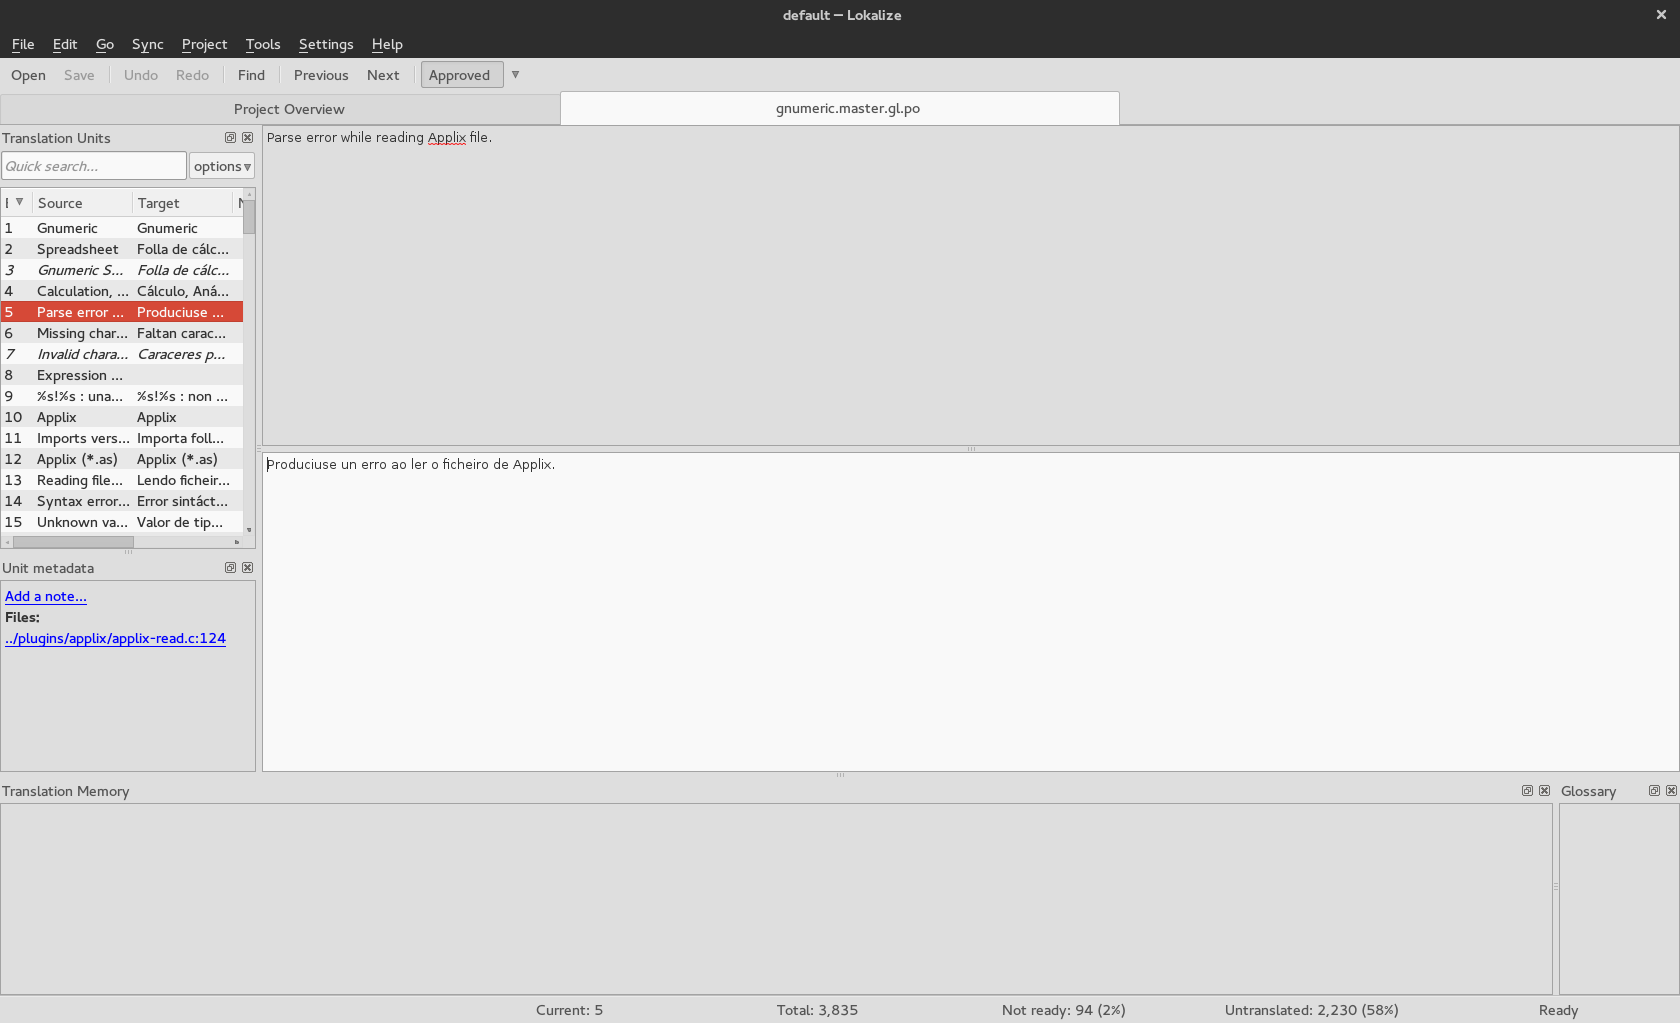
\includegraphics[width=\textwidth]{img/captura_lokalize.png}
    \caption{Interface de Lokalize}
    \label{fig:lokalize}
\end{figure}

En canto á interface, o programa permite abrir varios ficheiros cada un na súa lapela. Como se pode ver na Figura~\ref{fig:lokalize}, a vista de tradución está centrada no panel de edición, onde aparecen tanto a cadea orixinal como a cadea para traducir. Na columna da esquerda podemos ver a lista de cadeas, onde se amosan os primeiros caracteres da cadea orixinal e da tradución e o estado desta tradución. Ademais, tamén se pode ver o contexto da tradución, engadir un novo comentario e ver en que ficheiros estaba dita tradución. Por último, tamén podemos ver na parte inferior a memoria de tradución e o glosario.

\subsection{Virtaal}

Virtaal é unha ferramenta CAT\cite{website:virtaalweb} creada por Translate House\footnote{Compañía que surxiu a partir dunha comunidade de tradutores de Sudáfrica e que está especializada na creación de ferramentas e bibliotecas para axudar a tradución.} As características máis destacables son a incorporación de suxestión a tradución, comprobación da calidade das tradución e, sobre todo, a capacidade de abrir unha gran variedade de formatos a través da biblioteca Translate Toolkit.

\begin{figure}[h]
    \centering
    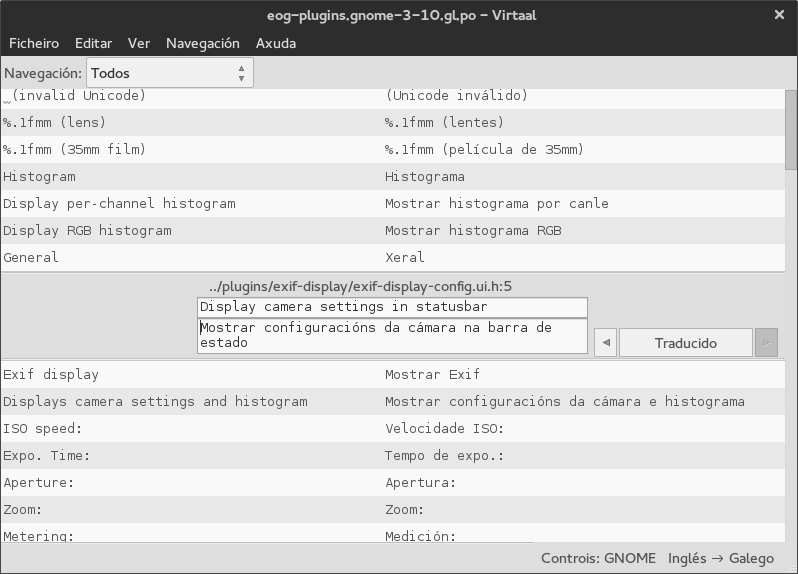
\includegraphics[width=\textwidth]{img/captura_virtaal.png}
    \caption{Interface de Virtaal}
    \label{fig:virtaal}
\end{figure}

Como se pode ver na Figura~\ref{fig:virtaal}, a interface é minimalista e moi centrada na tradución. A diferenza dos casos anteriores, trátase dunha interface fixa e que integra a lista das mensaxes coa edición da propia mensaxe. Tamén se indican posibles fallos que poida ter a tradución, como falta de puntos ó final, ausencia de marcadores de formato, etc.

\subsection{OmegaT}
Ferramenta CAT\cite{website:omegat} lanzada no ano 2001 e pensada fundamentalmente para tradutores profesionais. Ten soporte para o uso de memoria de tradución, glosario, tradución directa entre outras cousas. Destaca a gran cantidade de formatos que pode empregar.

\begin{figure}[h]
    \centering
    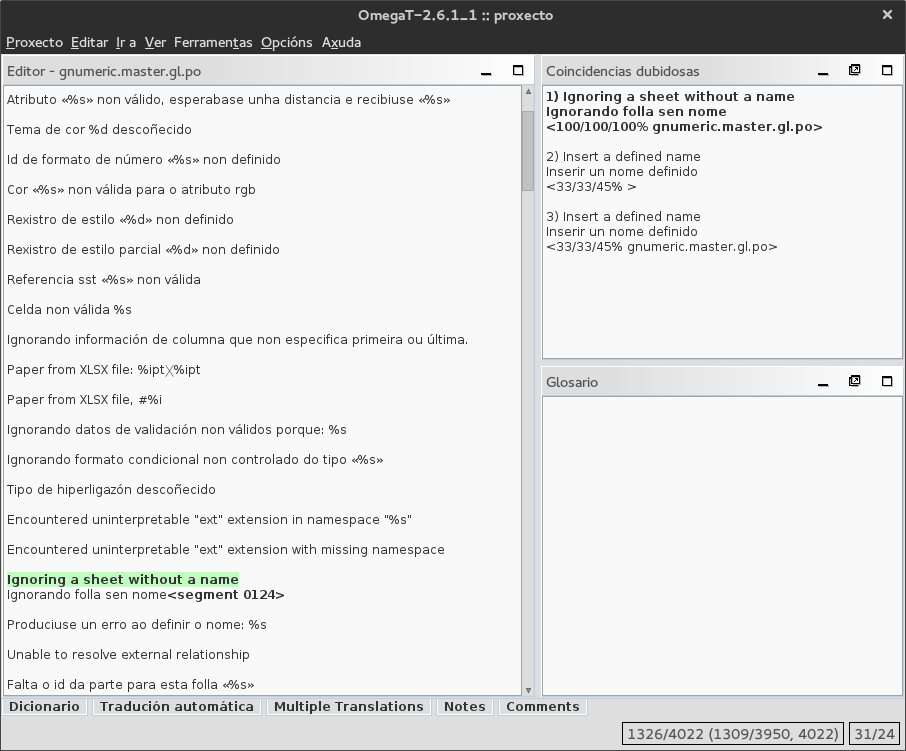
\includegraphics[width=\textwidth]{img/captura_omegat.png}
    \caption{Interface de OmegaT}
    \label{fig:omegat}
\end{figure}

A interface de OmegaT dista bastante do resto de programas. Como amosa a Figura~\ref{fig:omegat}, non existe o concepto de lista de mensaxes para traducir. O documento amósase como unha sucesión de cadea e se facemos clic encima dunha, permitiranos traducila. Trátase dun programa moi usado para a tradución tanto profesional como amateur.

\subsection{Google Translation Toolkit}
É a ferramenta CAT desenvolvida por Google e lanzada no ano 2008. A diferenza dos aplicativos analizados anteriormente, esta trátase unha solución puramente web. Entre as súas principais características, encóntrase a posibilidade de facer tradución automática empregando Google Translator, o uso de memorias de tradución compartidas, glosarios, soporte de etiquetas HTML, entre outros, e atallos de teclado. Ten soporte para varios formatos, como ficheiros PO, documentos de Microsoft Word, de LibreOffice ou mesmo artigos da Wikipedia.

\begin{figure}[h]
    \centering
    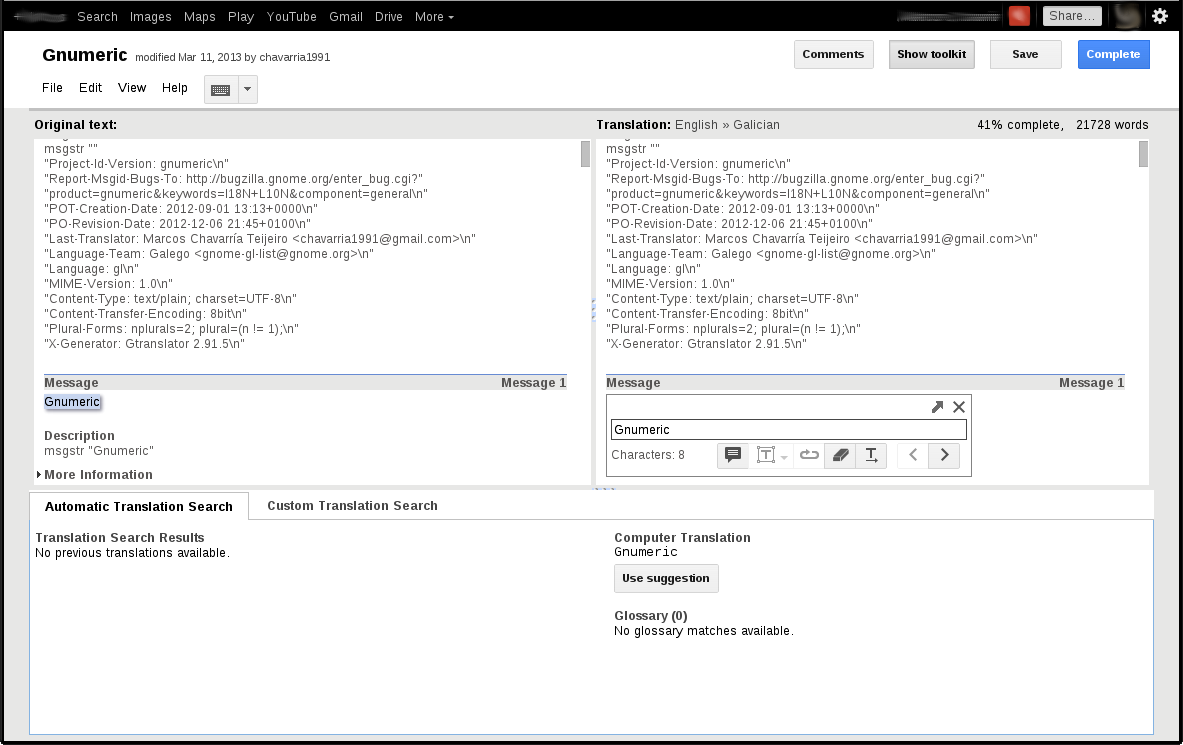
\includegraphics[width=\textwidth]{img/captura_googletranslationtoolkit.png}
    \caption{Interface de Google Translation Toolkit}
    \label{fig:translatetoolkit}
\end{figure}

Como se pode ver na Figura~\ref{fig:translatetoolkit}, na interface mestúrase a lista de cadeas co seu cadro de edición. Ademais, emprega unha interface semellante á do resto de ferramentas ofimáticas de Google, temos botóns para autocompletar etiquetas e para avanzar a seguinte tradución. Aínda que foi pensado para a tradución colaborativa de documentos de ONGs e artigos da Wikipedia, na actualidade emprégase maioritariamente para a tradución de proxectos comerciais.


\subsection{Transifex}
Trátase dunha plataforma que xurdiu a partir dun proxecto do Google Summer of Code do ano 2007 que pretendía crear unha plataforma online máis amigable que o Damned Lies de GNOME que naquel momento tamén empregaba Fedora unha distribución de GNU/Linux. Trátase dunha solución de pago con plans que van dende os 19 ós 300 dólares. Non obstante, os proxectos de código aberto poden usar o servizo de forma gratuíta e dispón dun período de mostra 30 días. As súas principais características son a posibilidade de descargar o documento e volvelo subir para poder traducilo con outra ferramenta CAT, editor online, memoria de tradución e unha API que permite integralo con outros servizos. Ademais, tamén soporta unha gran variedade de formatos, entre os que se atopan os ficheiros PO, DTD de Mozilla ou XML, entre outros.

\begin{figure}[h]
    \centering
    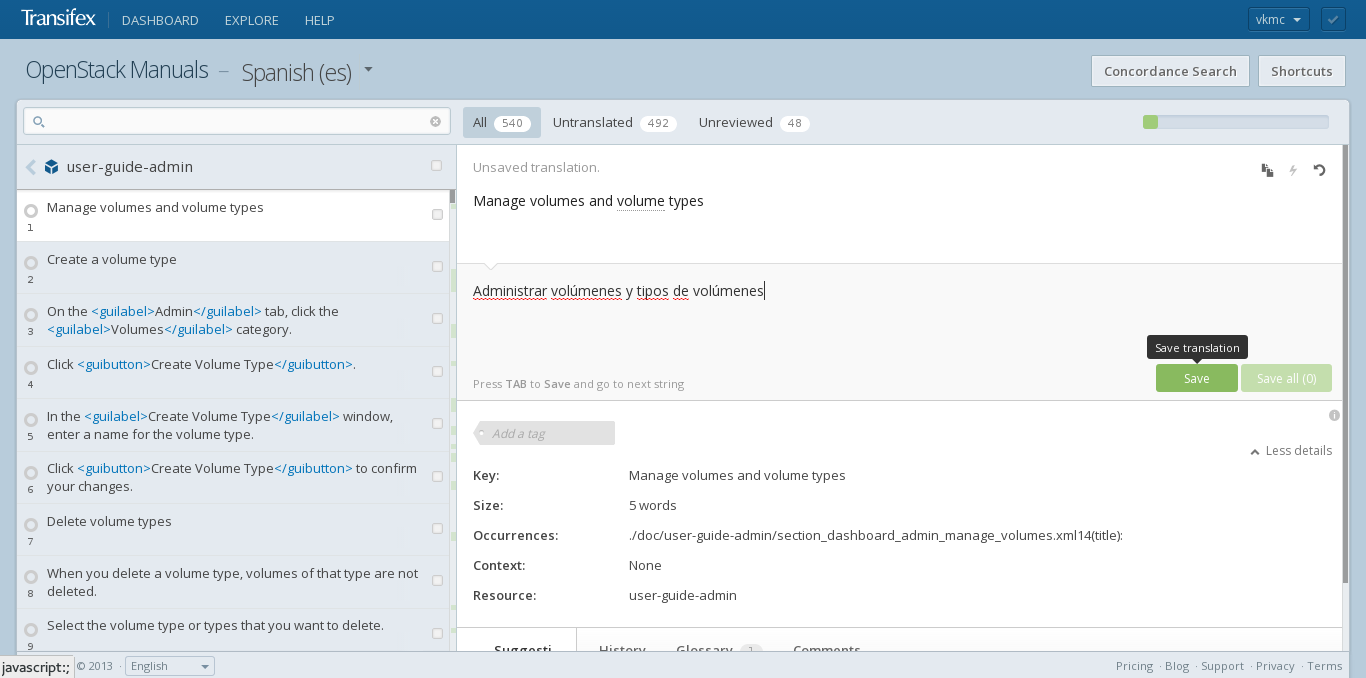
\includegraphics[width=\textwidth]{img/captura_transifex.png}
    \caption{Interface de Transifex}
    \label{fig:transifex}
\end{figure}

A interface de Transifex, como ser pode ver na Figura~\ref{fig:transifex}, separa a lista de cadeas do cadro de edición. No cadro de edición temos a posibilidade de consultar a memoria de tradución ou o glosario. O programa tamén incorpora resaltado de sintaxe.

\subsection{Outras ferramentas}
Existen moitas máis ferramentas CAT no mercado. De feito, segundo unha enquisa \cite{article:2006survey} elaborada polo Imperial College London a cerca de 900 tradutores profesionais de 54 países diferentes, OmegaT é o único programa que aparece na enquisa (cun 7\% de usuarios) de todos os programas anteriormente citados. As ferramentas máis usadas son ferramentas para Microsoft Windows e ferramentas con licenzas privativas e usualmente moi caras. Algunhas destas ferramentas son TRADOS, Wordfast, DejaVu SDLX ou STAR Transit. Na Figura~\ref{fig:enquisa2006} podemos ver unha gráfica coas ferramentas máis empregadas segundo este estudo.

\begin{figure}[h]
    \centering
    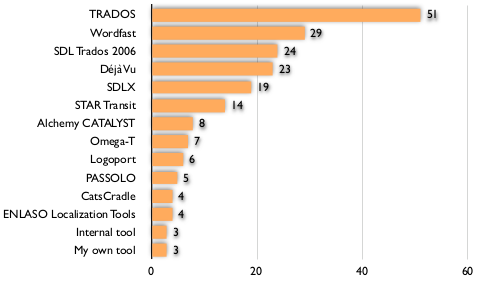
\includegraphics[width=0.7\textwidth]{img/grafico_uso_cat_enquisa2006.png}
    \caption{Ferramentas CAT máis empregadas segundo \cite{article:2006survey}.}
    \label{fig:enquisa2006}
\end{figure}

Hai que ter tamén en conta que se trata dun estudo bastante antigo, polo que algunhas das ferramentas analizadas aínda non existían. Por exemplo, a enquisa cita a ferramenta KBabel, que é a ferramenta de KDE na que está baseada Lokalize, pero con menos dun 2\% de usuarios.


\section{Características xenéricas das ferramentas CAT}

Algunhas das características que aparecen de forma recorrente en todas as ferramentas analizadas son as seguintes:

\subsection{Memoria de Tradución}
Unha memoria de tradución é unha base de datos composta de textos orixinais acompañados das súas traducións. Estes textos almacénanse en segmentos onde a separación entre segmentos vén dada por signos de puntuación ou o cambio de parágrafo, sendo esta última forma a máis frecuente.

A principal función dunha memoria de tradución é a extracción de coincidencias totais ou parciais. Os programas que teñen esta característica buscan na base de datos un segmento que coincida de forma exacta ou parcial coa cadea que se está a traducir e móstrase este segmento como suxestión. Xunto coa suxestión tamén se amosa o grao de proximidade entre a cadea a traducir e para cadea da memoria de tradución.

Existe un formato estándar de compartición de memorias de tradución de nome Translation Memory eXchange (TMX) e plataformas online que almacenan gran cantidade de cadeas e, polo tanto, hai máis posibilidade de obter unha mellor coincidencia. O software Amagama creado por Translate House, os creadores de Virtaal, é un exemplo de memoria de tradución online.

\subsection{Glosario}
Un glosario é unha base de datos de termos xunto cunha ou varias traducións aceptadas. Diferénciase da memoria de tradución en que só se proporciona a tradución a termos e non a cadeas completas. De igual forma que no caso das memorias de tradución, existe un formato estándar de para a compartición de glosarios de nome TermBase eXchange (TBX) e plataformas online para almacenar os glosarios.


\subsection{Previsualización}
As funcións de previsualización permítenlle ó tradutor ver como vai quedar a cadea traducida no programa final.

Os programadores e deseñadores fan as interfaces tendo en conta a lingua orixinal e non ningunha das traducións, polo que se unha tradución é moito máis longa cá orixinal pode verse mal no programa final.

Para conseguir esta característica pódense empregar varias técnicas:

\begin{itemize}
  \item \textbf{Programa orixinal.} Esta técnica que se pode empregar en calquera cadea consiste en compilar o ficheiro PO e executar o programa final con ese ficheiro PO. Desta poderemos ver como queda a nosa tradución para o usuario final. A desvantaxe deste método consiste en que teremos que saber en que parte do programa se emprega a cadea que queremos previsualizar. Este método é empregado por Lokalize que permite a definición de scripts para a previsualización de cadeas.

  \item \textbf{Renderizado de interfaces de usuario en XML.} Nas bibliotecas de interfaces modernas existe a posibilidade de definir interfaces en ficheiros XML e despois renderizalas. Neste caso as cadeas para traducir van nestes arquivos e sería posible renderizar esta interface coa tradución que estamos a realizar. Este método, aínda que si que amosaría a pantalla onde aparece a cadea actual, só é válido para as cadeas que proveñen destes ficheiros XML e non as definidas da forma tradicional. Un exemplo deste método pódese ver na rede no aplicativo Deckard\footnote{\href{http://deckard.malizor.org/}{deckard.malizor.org}} que permite ver as traducións de aplicativos de GNOME.
\end{itemize}


\subsection{Tradución Directa}
A tradución de cadeas de forma automática empregando algoritmos deseñados para tal proceso e que empregan grandes bases de datos aloxadas, xeralmente en internet. Tanto Google como Microsoft teñen os seus produtos corporativos que fan traducións e existen alternativas libres como OpenTrad ou Apertium. Estas traducións, aínda que válidas, acostuman ser de baixa calidade, polo que necesitan unha revisión.

        \chapter{Fundamentos Tecnolóxicos}

Neste capítulo detallaremos os compoñentes tecnolóxicos que empregamos para levar a cabo este proxecto. Primeiro falaremos das ferramentas empregadas e despois das diferentes bibliotecas que usamos no programa.

\section{Ferramentas empregadas}

\paragraph{Vala} É unha linguaxe de programación orientada a obxectos creada por GNOME para acercar a linguaxe de programación C as características das linguaxes de programación modernas. Emprega C xunto coa biblioteca GObject como linguaxe intermedio. Esta linguaxe cunha sintaxe moi parecida a C\# incorpora características como o uso e funcións anónimas, bucles foreach, xestión automática de memoria ou o manexo de excepcións.


 \paragraph{Autotools} Tamén coñecidas como \emph{GNU build system} son un conxunto de ferramentas que permiten permitir a configuración e compilación de programas portables a varias plataformas UNIX.

 \paragraph{Git} É un sistema de control de versións distribuído escrito por Linus Torbards e usado, entre outros moitos proxectos, para xestionar o desenvolvemento de Linux (o kernel). Trátase dunha das solucións de control de versións máis empregada na actualidade pois é moito máis rápida que as outras existentes e, ao ser distribuída, permite traballar ser conexión a internet.

 \paragraph{GitHub} Unha plataforma de almacenamento de proxectos empregando o sistema de control de versións Git. Permite subir proxectos Open Source de forma gratuíta os seus servidores. Conta ademais con ferramentas para a creación de Wikis relacionadas cos proxectos e incorpora un xestor de fallos.

 \paragraph{Listas de Correo} As listas de correo son un medio de comunicación asíncrona moi usadas no mundo do desenvolvemento software. Os usuarios escriben un correo electrónico a un enderezo especial que reenvia dito correo a todos os usuarios subscritos as listas. Ademais os correos enviados a lista son almacenados nun historial para a súa posterior consulta.

 \paragraph{IRC (Internet Relay Chat)} É un protocolo de comunicación entre usuarios creado no ano 1988. É amplamente usado no mundo do desenrolo software como unha ferramenta rápida para consultar dubidas entre desenvolvedores. Existen múltiples clientes dispoñibles para case calquera plataforma. En concreto empregouse o programa XChat.

 \paragraph{JHBuild} Unha serie de scripts que permiten a descarga automática do código fonte dun proxecto e das súas dependencias e a instalación destes proxectos dentro dun entorno separado do resto do sistema. Desta forma os desenvolvedores poden traballar coas últimas versións das bibliotecas que tenden a ser inestables sen ter que usalas en todo os seu sistema.

\paragraph{Glade} Unha ferramenta para a creación de interfaces de usuario con GTK+ as interfaces creadas expórtanse en ficheiros con formato XML.

\paragraph{Dia} É un programa para a creación de diagramas de todo tipo. Ten un paquete para facer diagramas UML.

\paragraph{JSON} É un formato para o intercambio de datos. Acrónimo de JavaScript Object Notation, trátase dun subconxunto da notación para definir obxectos en JavaScript. Para poder analizar este formato no noso programa empregaremos a biblioteca JSON-GLib.

\paragraph{GDB} GNU Project debugger. É o depurador estándar para o proxecto GNU. Permite a execución paso a paso, monitorizar e alterar o valor das variables entre outras moitas características.

\paragraph{\LaTeX} É un sistema de composición de textos. Creado por Leslie Lamport como un gran conxunto de macros de \TeX para facilitar o seu uso, produce documentos de gran calidade con pouco esforzo. Permite incluír dentro dos textos formulas matemáticas, fragmentos de códigos ou figuras, entre outros.

\section{Bibliotecas empregadas}

\paragraph{GLib} É unha biblioteca de propósito xeral creada por GNOME a partir de 5 librerías, GObject, GLib, GModule, GThread e GIO.

\emph{GObject} incorpora características da orientación a obxectos a linguaxe de programación C, como pode ser a creación de clases, herdanza ou as propiedades entre outras. \emph{GLib} constitúe un conxunto de tipos básicos empregados no resto de bibliotecas. \emph{GModule} permite a carga de módulos ou extensións de forma dinámica. Por último, \emph{GThread} é unha biblioteca de xestión de fíos de execución e \emph{GIO} é unha biblioteca pensada para facilitar a entrada e saída nos programas.

Esta biblioteca constitúe unha dependencia básica en todas os aplicativos feitos co \emph{stack} de GNOME e, de feito, é unha dependencia de case todas as demais bibliotecas que empregamos.

\paragraph{GTK+} Biblioteca multiplataforma para a creación de interfaces gráficas de usuario desenvolvida por GNOME. Incorpora unha serie de widgets para a creación de programas tanto grandes como pequenos. Está escrita en C pero existen bindings para moitas linguaxes.

As interfaces gráficas pódense crear de forma programática ou cargando un ficheiro XML. Aínda que pode parecer moito máis traballoso a creación dun ficheiro XML con ese propósito, a existencia de ferramentas como Glade\footnote{\href{http://glade.gnome.org}{glade.gnome.org}}.

\paragraph{LibGee} Trátase dunha biblioteca que fornece a GObject de estruturas de datos comunmente usadas como listas, táboas hash ou conxuntos entre outros.

\paragraph{LibPeas} LibPeas é un motor de plugins para GObject. Escrito orixinalmente para GEdit permite as aplicacións estenderse a través dun sistema de plugins.

\paragraph{GettextPo} Trátase dunha biblioteca que analiza ficheiros GNU Gettext PO. Esta biblioteca está implementada en C e non existen bindings para Vala polo que teremos que facelos nós.

\paragraph{GTKSourceView} Esta biblioteca estende o \emph{widget} de GTK+ GtkTextView, que permite a visualización de textos, para incorporarlle certas características avanzadas como a xestión de cambios permitindo desfacer e refacer ou o resaltado da sintaxe.

\paragraph{JSON-GLib} É unha biblioteca para a análise de cadeas de texto en formato JSON.

        \chapter{Metodoloxía}

Nesta sección descríbese a metodoloxía levada a cabo para a realización deste proxecto. Unha metodoloxía é un conxunto de métodos ou prácticas empregadas para a realización dunha tarefa, neste caso a análise, deseño e implementación dunha nova ferramenta CAT para o proxecto GNOME. Escolleuse unha metodoloxía áxil de ciclo incremental. Moitas das prácticas que se tomaron son collidas da metodoloxía eXtreme Programming.

\section{eXtreme Programming}

Foi creada por Kent Beck no ano 1999\cite{book:extremeprogramming}, e trátase dun dos máis destacados métodos de desenvolvemento áxil. eXtreme Programming (a partir de agora XP) avoga por ciclos de desenvolvemento moi curtos e elimina os roles clásicos de analista, deseñador e programador. Todo equipo participa en todas as partes do desenvolvemento. Desta forma, Beck define uns valores fundamentais da metodoloxía e unhas prácticas que axudan a adoptar estes valores.

\subsection{Valores de eXtreme Programming}

\subsubsection{Comunicación}
É o primeiro valor de XP. Segundo esta metodoloxía, os problemas nos proxectos poden ser traducidos a alguén que non falou con outra persoa sobre algo importante do proxecto. Esta mala comunicación non sucede por casualidade e é debido frecuentemente ás malas prácticas. Para solucionar isto, XP inclúe prácticas nas que é necesaria a comunicación para levalas a cabo. Ademais a figura do \emph{coach} serve para mellorar a comunicación daquelas persoas que non o están facendo ben.

\subsubsection{Simplicidade}

A simplicidade non é unha tarefa sinxela. XP fai unha aposta e invita ao programador a pensar no que o proxecto necesita hoxe e non no que vai necesitar nun futuro. Para manter esta simplicidade ao longo do tempo, é frecuente a súa refactorización. A simplificación do deseño e da implementación axiliza tanto o desenvolvemento como o mantemento. A simplicidade require \textbf{comunicación}, pois canto máis comunicación teñamos por parte do cliente máis sinxelo poderemos facer o sistema, e canto máis simple sexa o sistema, menos comunicación será necesaria para explicar o sistema.

\subsubsection{Retroalimentación}
A retroalimentación ou feedback é fundamental nesta metodoloxía. Pode actuar en varias escalas de tempo. Obtemos feedback en cuestión de minutos ou días de parte dos test do sistema, das peticións dos clientes ou do director do proxecto. Tamén obtemos feedback ó longo dos meses cando o usuario pode analizar as características que implementamos. Neste sentido XP aposta por unha posta rápida en produción, de forma que teñamos sistemas en desenvolvemento e en produción de forma paralela. Con isto melloramos o sistema, xa que imos obtendo as opinións dos usuarios das decisións que xa tomamos e os erros cometidos non se volven repetir.

\subsubsection{Coraxe}
O coraxe é unha parte inherente á metodoloxía. É necesario para tirar o traballo de varios días e volver empezar debido a cambios nos requisitos ou aparición de fallos estruturais. É necesario para ser persistente coa resolución dun problema, as cousas que non se dan resolto un día en horas, pódense resolver ó día seguinte en cuestión de minutos. O coraxe non é útil sen os tres primeiros valores. Cunha boa comunicación existe a posibilidade de facer experimentos con máis risco. A simplicidade permítelle ó programador coñecer mellor o código e, polo tanto, ser máis valente á hora de facer cambios. A retroalimentación axuda a que alguén se sinta máis seguro ao facer un cambio.

\subsubsection{Respecto}
Por último, é necesario respecto. É necesario que os integrantes do equipo se preocupen polo resto de membros e polo que están facendo. Ademais o equipo debe preocuparse polo propio proxecto. Para que XP funcione os programadores débense sentir parte do proxecto e ter un feedback positivo ao respecto.

\subsection{Prácticas recomendadas por eXtreme Programming}

\subsubsection{O Xogo da Planificación}
A planificación é un diálogo entre a xente do negocio e o equipo técnico. Mentres a parte de negocio decide a importancia dun problema, a prioridade da implementación dunha característica ou outra, a composición das entregas ou as datas das mesmas, o equipo técnico é capaz de estimar canto tempo leva implementar unha característica, ten a capacidade de explicar as consecuencias de certa decisión, sabe como organizarse para levar a cabo unha tarefa e pode facer unha planificación máis detallada.

\subsubsection{Entregas Pequenas}
As entregas ou \emph{releases} deben ser o máis pequenas posibles e conter os requerimentos máis valiosos. Aínda así, cada release debe ser autocontida e non ter características implementadas a medias solo para facer o ciclo de entregas máis curto.

\subsubsection{Metáfora}
Cada proxecto feito con XP ten unha metáfora. Unha metáfora é un símil sinxelo de como está composto o sistema. É útil para que os membros do equipo teñan unha visión global do que están facendo e que membros non técnicos do equipo poidan entendelo.

Outras metodoloxías chámanlle a isto \textbf{arquitectura}. O problema con empregar o termino arquitectura é que unha arquitectura non ten necesariamente un sentido de cohesión.

\subsubsection{Deseño simple}
Todos os deseños deben, executar todos os tests, non ter código duplicado, ter o menor número de clases e métodos e todas as partes son importantes para os programadores. Con esta filosofía XP intenta facer un deseño simple para as necesidades actuais do programa. Desta forma, a implementación será máis rápida e o tempo de aprendizaxe para os outros membros do equipo será máis curto.

\subsubsection{Testing}
Calquera característica incorporada que non inclúa un test, simplemente non existe. Os programadores inclúen test de unidade para as novas funcionalidades e os clientes crean test funcionales de como esperan que o programa funciona. Ambos test forman parte do código do programa. Non é necesario escribir test para cada método pero si para cada método que se expoña.

\subsubsection{Refactorización}
Cando é necesario implementar unha nova característica no programa, os programadores pregúntanse se existe unha forma simple de implementala e implementana. Despois analizan o código para ver se existe unha forma de facelo de forma máis simple e que siga executando correctamente todos os tests. Esto chamase refactorizar.

É obvio que traballando desta forma emprégase moito máis tempo do necesario para a implementación de cada característica, pero desta forma poderemos engadir a seguinte característica nunha cantidade razoable de tempo.

\subsubsection{Programación por parellas}
Todo o código en produción é escrito por parellas de programadores con diferentes roles. Por un lado un dos programadores pensara de forma específica como implementar un certo método, mentres o outro pensará dun xeito máis global e estratéxico. Estas parellas cambian continuamente.

\subsubsection{Pertenza Colectiva}
En XP o código pertence a todo o equipo e se unha persoa ten oportunidade de engadir algo de valor a algún fragmento de código ten que facelo nalgún momento. Desta forma todo o mundo ten responsabilidade sobre todo o sistema e, aínda que non todo o mundo coñece cada parte de forma igual, todo o mundo coñece algo de cada parte de forma que son capaces de facer modificacións satisfactorias.

Isto contrasta coas prácticas doutras metodoloxías onde o código escrito por unha persoa só pertence a esa persoa e para engadir nova funcionalidade é necesario facer unha petición a dito programador. Esta práctica pode facer máis lento o desenvolvemento e diminúe o factor camión\footnote{\href{http://en.wikipedia.org/wiki/Bus\_factor}{Truck Factor}: O numero de membros dun equipo dentro dun proxecto, que no caso de seren atropellados por un camión, o proxecto non podería completarse.}.

\subsubsection{Integración Continua}
Os test son executados con cada cambio e, soamente se todos os test son executados correctamente, sóbense os cambios ao produto final. É importante executar os test a cada cambio xa que así saberemos a que se debe o fallo e quen ten que corrixilo. Se para implementar unha característica os seus desenvolvedores non son capaces de que todos os tests funcionen, probablemente necesiten volver a empezar pois non tiñan os coñecementos necesarios para implemementala. 

\subsubsection{Semana de 40 horas}
XP establece unha xornada laboral de 8 horas e 5 días á semana. Para esta metodoloxía é importante que os programadores estean frescos e inspirados cada maña e con xornadas largas de traballo dita tarefa é imposible. O descanso é algo fundamental para poder ter boas ideas.

\subsubsection{Cliente no sitio}
Un cliente do proxecto, é dicir, unha persoa que realmente vaia usalo cando estea en produción, debe sentarse xunto ó equipo e poder responder preguntas e resolver disputas entre membros do equipo.

\subsubsection{Estándares de programación}
Cando se traballa cambiando de parellas cada pouco tempo e facendo refactorizacións continuas, cómpre que todo o equipo siga uns estándares de programación. Isto é, un mesmo estilo de código e unha mesma forma de facer certas cousas.

\section{Metodoloxía seguida}

Dentro das prácticas e valores suxeridos por eXtreme Programming seguimos un subconxunto do mesmo. Moitas das prácticas non se puideron levar a cabo debido a que se tratada dun proxecto dunha persoa.

\paragraph{Pertenza Colectiva} O programa que estamos facendo é software libre e polo tanto o seu código está dispoñible a todo aquel que queira melloralo. En concreto, o noso programa está subido á plataforma GitHub. Calquera persoa pode enviar cambios que poden ser integrados no programa ou reportar fallos.

\paragraph{Estándares de Programación} Na elaboración do programa intentamos seguir un estilo de código fixo en todos os ficheiros. Desta forma facilitamos aos novos desenvolvedores a lectura do código do noso programa.

\paragraph{Semana de 40 horas} Durante a elaboración do programa as horas diarias dedicadas ao programa foron aproximadamente cinco. Pensamos que desta forma o programador tería a mente máis descansada para poder programar.

\paragraph{Deseño Simple} Intentamos solucionar os problemas empregando un deseño simple, tendo en algunhas ocasións que refactorizar gran parte do código.

\paragraph{Cliente no sitio} Os clientes do programa, é dicir, os tradutores de GNOME, tiveron sempre a posibilidade de instalar o programa e comentar, ben a través do blogue, no xestor de fallos que incorpora GitHub, ou vía email as melloras que lles gustaría incorporar ao programa.

        \chapter{Planificación e Seguimento}

A elaboración deste proxecto levouse a cabo durante catro periodos de tempo diferenciados e separados no tempo:

\begin{itemize}
  \item O verán do ano 2013 como parte do programa GSoC.
  \item O primeiro cuatrimestre do curso 2013/2014.
  \item O verán do ano 2014 novamento como parte do GSoC.
  \item O segundo cuatrimestre do curso 2014/2015.
\end{itemize}

Neste cápitulo trataremos a planificación do proxecto e como se levou a cabo neses catro períodos de tempo.

\section{Google Summer of Code 2013}
O tempo de programación do Google Summer of Code son aproximadamente 4 meses, un total de 15 semanas. Durante a edición de 2013 planificouse qeu se ía traballar 13 semanas. As dúas semanas restantes correponden a asistencia a GUADEC e ao comezo do ano lectivo universitario 2013/2014. Contase traballar aproximadamente 5 horas diarias polo que dá un total de 325 horas.

O programa GSoC pide os participantes reportes periodicos en forma de artigos en blogs así que estas serán as nosas iteracións a través das cales iremos recibindo feedback por parte dos futuros usuarios do aplicativo. En función deste feedback iremos modificando o programa. Neste caso empregouse un blog personal creado con anterioridade e de nome \href{http://aquelando.info}{Aquelando.info}. As publicacións deste blog así como as de moitos desenvolvedores do proxecto GNOME están ligadas con Planet GNOME, que é un agregador de blogs, polo que a súa difusión é moi alta. A perioricidade das publicacións e polo tanto das iteracións variará dunha a outra pero é de entre dúas e tres semanas.

Durante este GSoC fixeronse 5 iteracións que explicamos a continuación.

\subsection{Primeira Iteración: Análise, deseño xenérico e inicio da implementación}

A primeira iteración iniciouse o 13 de Xuño e rematouse o 30 de Xuño. O tratarse da primeira iteración dun programa fíxose unha analise das necesidades e un deseño xenerico da estrutura do programa.

\subsubsection{Análise e deseño}
Para o análise, instalamos e estudiamos algúns programas existentes e enviamos correos a listas de correo de equipos de tradución para obter ideas. Obtemos bastante resporta sobretodo por parte de xente do Proxecto Trasno. Unha vez que tiñamos claro que necesidades ten o noso programa fixemos un deseño xenerico da estrutura do programa. Este deseño saca a luz algúns conceptos que estarán presente durante toda a vida do programa como poden ser os \emph{consellos} e as \emph{pistas}.

\begin{figure}[h]
    \centering
    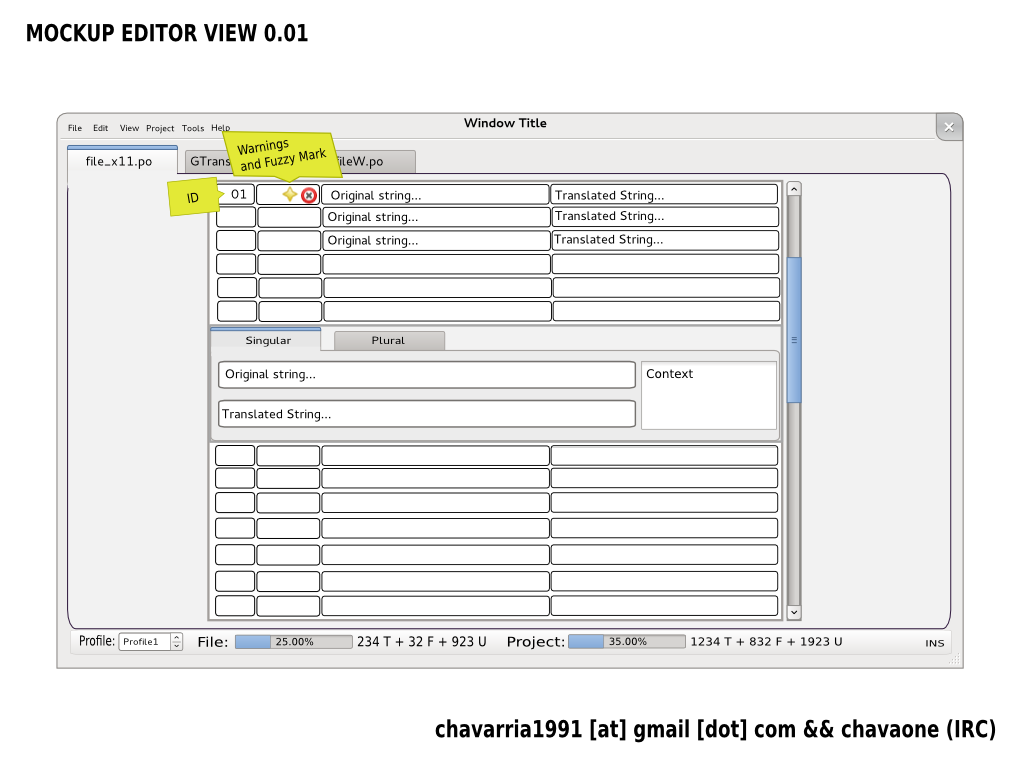
\includegraphics[width=\textwidth]{img/mockup_interface1.png}
    \caption{Mockup da interface presentado no reporte.}
    \label{fig:mockup_int1}
\end{figure}

Os consellos é un sistema lle amosa ao usuario posibles fallos que este tivo durante a tradución. Por outra pare as pistas son posibles traducións que se lle amosan ao usuario estas traducións poden vir de memorias de tradución, de outros linguaxes semellantes ou do propio ficheiro que se está a traducir, por exemplo.

Ademais tamén se fixo algun mockup da interface de usuario como o que se publicou no blog e se pode ver na Figura~\ref{fig:mockup_int1}. Estes deseños son bastante semellantes a interface do aplicativo Virtaal.

\subsubsection{Implementación da clase abstracta ficheiro}
Empeza a implementar parte do núcleo do sistema. Implementase unha clase abstracta ficheiro e unha clase \emph{DemoFile} que vai servir como mock para poder implementar a interface.

Esta clase implementase tendo en mente o concepto de extensibilidade xa que este programa aínda que se centra na edición de ficheiros PO por ser estes os "oficiais" de GNOME tamén queremos que este programa sexa útil para a comunidade de traductores en xeral.

\subsubsection{Reporte e feedback}
Escribironse un total de 3 reportes. Un\footnote{\href{http://aquelando.info/startinggsocprojec/}{Starting the GSoC Project!!}} facendo referencia as peticións obtidas por parte dos equipos de tradución e dous\footnote{\href{http://aquelando.info/valacat-some-design-aspects/}{ValaCAT. Some design aspects}}\footnote{\href{http://aquelando.info/valacat-some-design-aspects-part-2/}{ValaCAT. Some design aspects (Part 2)}} con algúns detalles que se tiveron en conta durante o deseño do programa. Houbo bastantes comentarios no blog e entre outras cousas os usuarios destacaron:

\begin{itemize}
  \item A importancia de non usar o patrón Singleton.
  \item Non facer os widgets dependentes da aplicación para que estos poidan ser reutilizados en outras aplicacións como Anjuta.
  \item Usar gettext-po para implementar os ficheiros po.
  \item Empregar unha interface máis semellante a anterior de GTranslator.
  \item Eliminar a columna de ID pois non se consider útil.
  \item Autoexpandir o tamaño dos campos cando as cadeas sexan grandes.
\end{itemize}

Con respecto a estas ideas modificouse a interface que se ía facer para buscar un deseño moi parecido ao de GTranslator empregando ingluso a mesma biblioteca GNOME Docking Library que permite modificar os bloques da interface. Ademais eliminouse por completo o ID da cadea da interface. En canto a biblioteca gettext-po xa tiñamos en mente empregala.

\subsubsection{Tarefas e seguimento}

As tarefas que se realizaron durante esta iteración foron as seguintes:

\begin{itemize}
  \item Análise de Requisitos
    \begin{itemize}
      \item Estudio de ferramentas existentes.
      \item Enviar correos a diferentes equipos de traductores.
      \item Analizar respostas dos equipos.
    \end{itemize}
  \item Deseño xenerico do aplicativo.
  \item Deseño e implementación do ficheiros xenérico.
  \item Escribir primeiros reportes.
\end{itemize}

Planificaronse un total de 50 horas e fixeronse 60 debido a ter que esperar por que os traductores deran as súas opinións.

\subsection{Segunda Iteración: Linguaxes, Filtros e Interface}

A segunda iteración durou dende o 1 de Xullo ata o 18 de Xullo. Nesta iteración profundizase no núcleo do sistema e empezamos a traballar na interface de ususario.

\subsubsection{Linguaxes}
Implementación da clase linguaxe e da clase forma plural. Fixemos un par de ficheiros con cada linguaxe e con cada forma plural existente. A idea detras destes ficheiros é engadir información adicional a cada linguaxe e a cada forma plural. 

Nas formas plurais incluimos unhas etiquetas para explicar en forma de texto a que corresponde cada tipo de plural. Por exemplo para os plurais do galego, a forma plural 0 tería unha etiqueta ``Singular (1 elemento)'' e a forma plural tería a forma ``Plural (0 ou máis de 1 elementos)''. Desta forma resultará máis sinxelo identificar cada forma plural e non ter que usar só o número.

\subsubsection{Filtros para as cadeas}
Os filtros para as cadeas corresponde a idea de que cada consello poda incluir a función de resaltar certas partes da mensaxe para reforzar a información que nos dá. Estos filtros funcionan como un patrón decorador que colocan uns tags html antes e despois da parte resaltada de forma que despois se poda parsear esta información e mostrala ao usuario cambiando os estilos.

\subsubsection{Interface de usuario}
Empezase a traballar na interface do usuario. Nesta iteración crease a estrutura xeral e os widget de listar mensaxes, de editar mensaxes e de mostar o contexto da mensaxe. O aspecto final da interface despois desta iteración pódese ver na Figura~\ref{fig:gsoc1_iter2_ui}.

\begin{figure}[h]
    \centering
    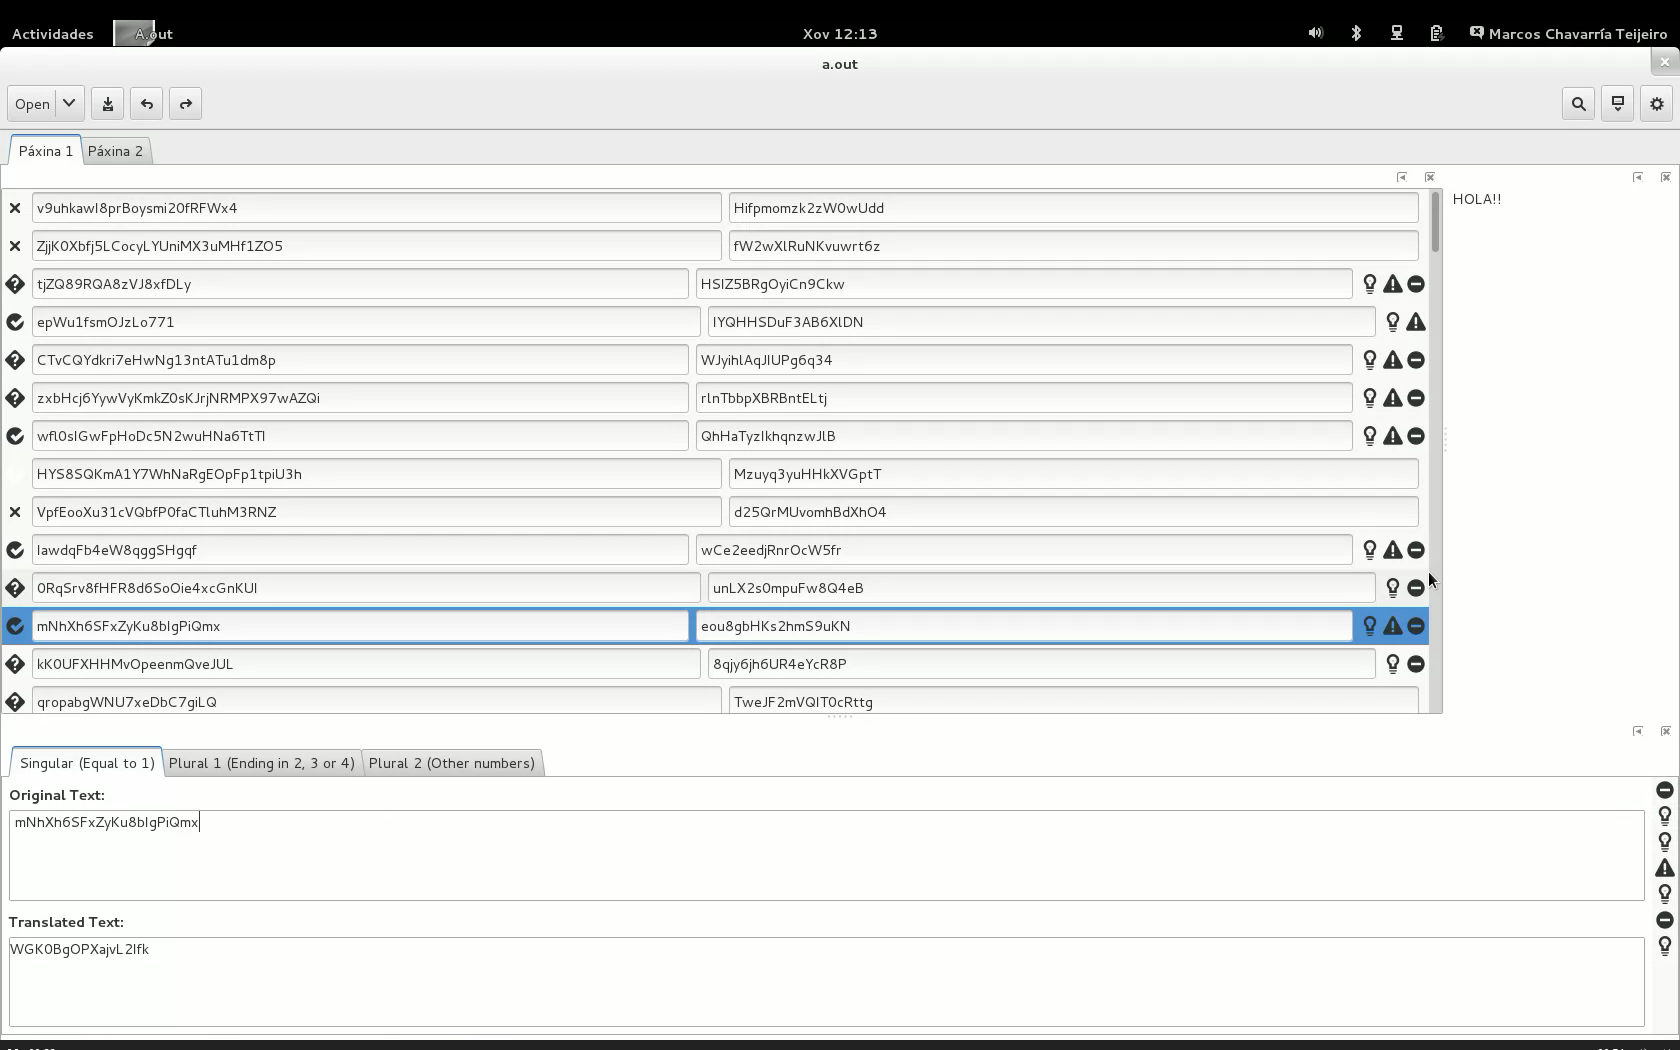
\includegraphics[width=0.8\textwidth]{img/gsoc1_it2_ui.png}
    \caption{Primeira implementación da interface.}
    \label{fig:gsoc1_iter2_ui}
\end{figure}

\subsubsection{Reporte e feedback}
Escribiuse un\footnote{\href{http://aquelando.info/valacat-application-current-status/}{ValaCAT application current status}} reporte onde se puxo un vídeo no que se amosaba o estado do programa e todas as caracteristicas implementadas. Recibimos un comentario preguntando para que sirven certas partes da aplicación que aparecen no vídeo e respondese explicando as ideas empregadas e reforzandoo con outro video centrado nesas partes.

\subsubsection{Tarefas e Seguimento}

As tarefas que realizamos durante esta iteración foron as seguintes:

\begin{itemize}
  \item Deseño e Implementación do módulo de Linguaxes.
    \begin{itemize}
      \item Creación dos ficheiros JSON coa lista de formas plurais e de linguaxes.
    \end{itemize}
  \item Interface de usuario.
    \begin{itemize}
      \item Implementación da lista de mensaxes.
      \item Implementación do editor de mensaxes.
      \item Implementación da barra de estado.
      \item Implementación da lapela xenerica.
      \item Implementación da lapela para ficheiros.
    \end{itemize}
  \item Creación do Makefile
  \item Creación de filtros para as cadeas.
  \item Escribir reportes.
\end{itemize}

Planificaronse un total de 70 horas para esta iteración e completaronse en 75 horas. Estas horas fixeronse traballando máis horas ao día polo que non supuxo un desvio. 

\subsection{Terceira Iteración: Interface, iteradores e buscas}

\subsubsection{Iteradores e Buscas}
Os iteradores son o sistema empregado para navegar a través das cadeas do documento. Construironse de forma qeu o usuario puidese navegar a través de todas as cadeas, das cadeas sin traducir ou das cadeas con tradución difusa. Ademais creouse o módulo para buscar texto no documento.

\subsubsection{Interface de usuario}
Seguimos traballando na interface de usuario. Cambiamos o widget de edición para empregar a biblioreca GtkSourceView que incorpora un widget que permite resaltado de sintaxe, de espacios en blanco entreo outros. Ademais empezamos a usar a clase GtkAplication e GtkAplicationWindow. Os filtros son substituidos por GtkTextTags que estan integrados dentro da librería GTK. Engadimos un dialogo para facer buscas onde se poden selecionar distintos parametros sobre qeu cadeas incluir nas búsquedas.

\begin{figure}[h]
    \centering
    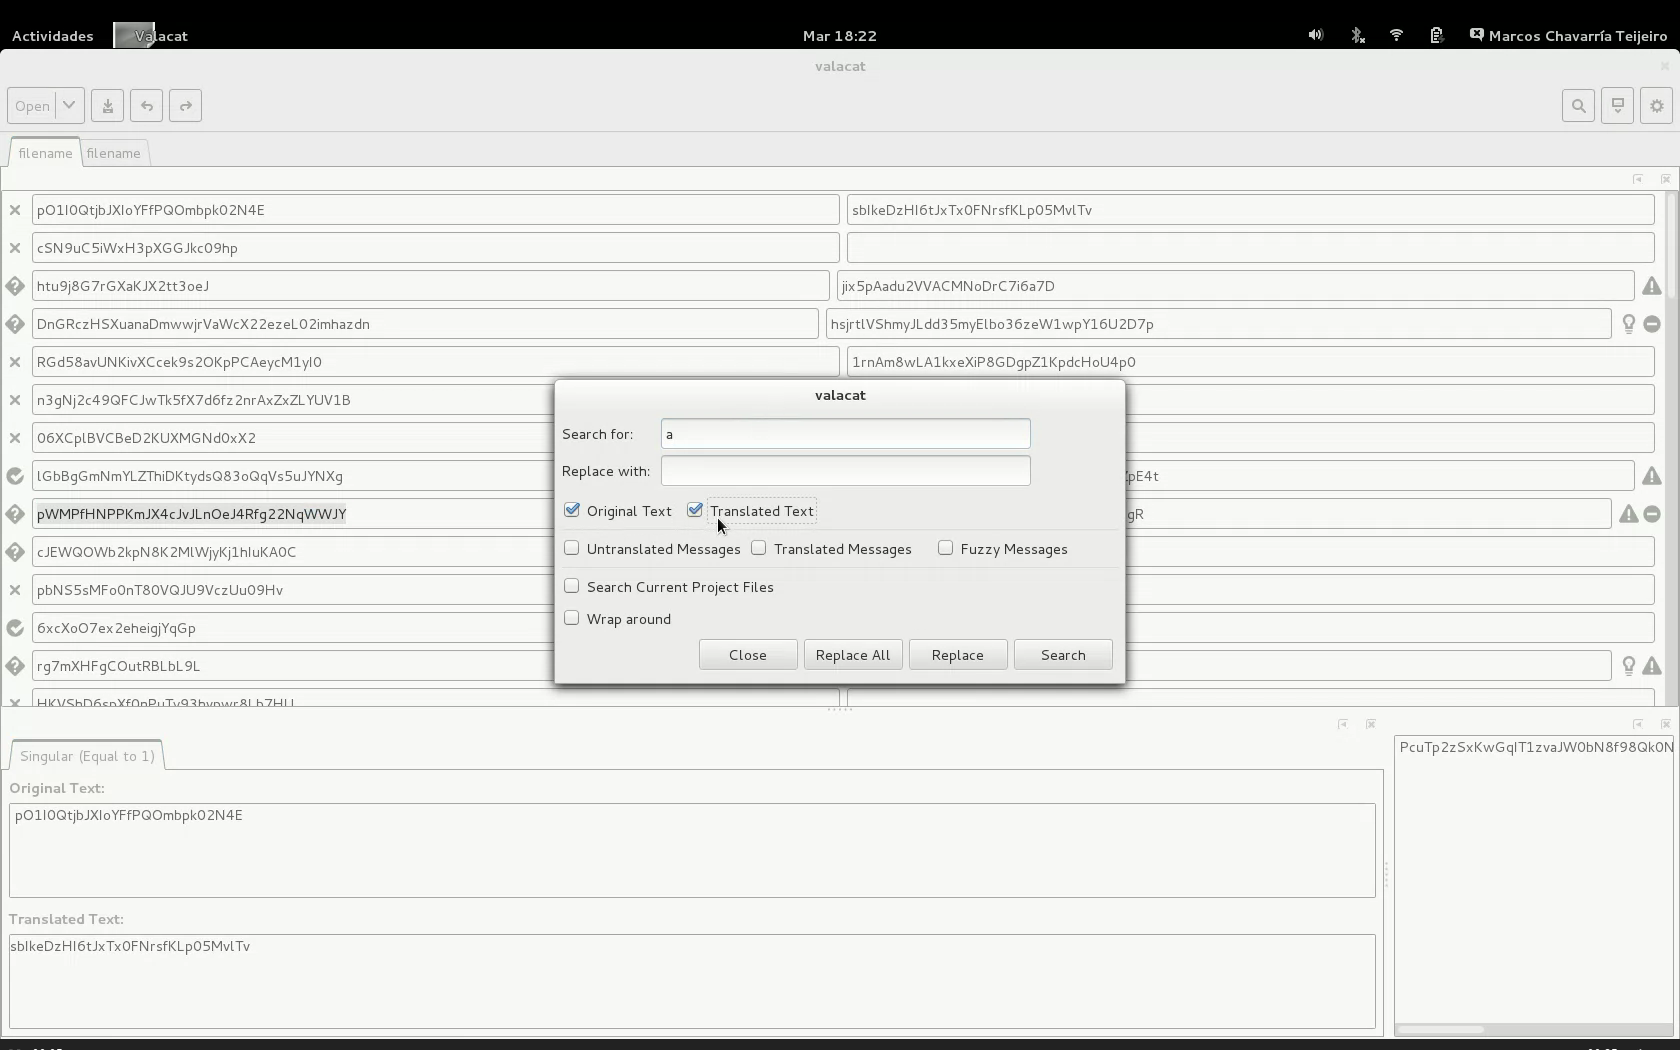
\includegraphics[width=0.8\textwidth]{img/gsoc1_it3_ui.png}
    \caption{Primeira implementación da interface.}
    \label{fig:gsoc1_iter3_ui}
\end{figure}

O aspecto que ten esta interface o finalizar esta iteración pódese ver na Figura~\ref{fig:gsoc1_iter3_ui}.

\subsubsection{Presentación GUADEC 2013 (Brno)}
A GUADEC e a xuntanza europea de desenvolvedores e usuarios de GNOME. Os participantes no GSoC están invitados a ir a dita reunión e expoñer o seu traballo nunha charla relámpago dun máximo de 3 minutos.

\begin{figure}[h!]
    \centering
    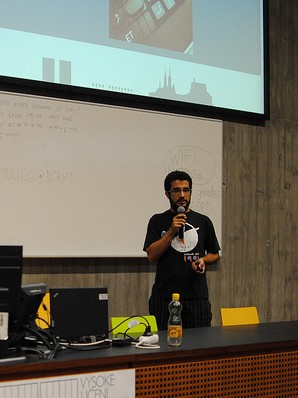
\includegraphics[width=0.275\textwidth]{img/guadec_2013_1.jpg}
    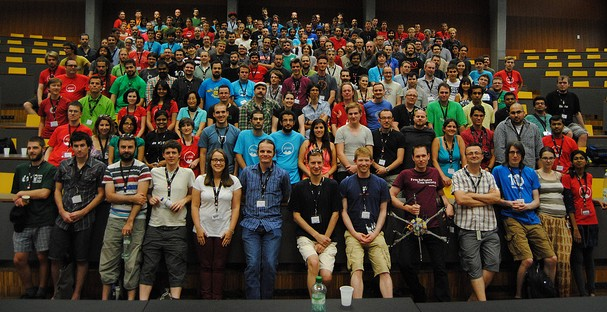
\includegraphics[width=0.715\textwidth]{img/guadec_2013_2.jpg}
    \caption{GUADEC 2013 (Brno)}
    \label{fig:guadec2012}
\end{figure}

Ademais de presentar o proxecto nesta xuntanza participei no evento como voluntario o que me permitiu coñecer a moita xente, algunha desa xente podo dicir que a día de hoxe son amigos meus.

\subsubsection{Reportes e Feedback}

A Fundación GNOME ponse en contacto conmigo a través do email para pedirme que, xa que esta vai ser o aplicativo oficial de GNOME, ten que ter a palabra GNOME no seu nome.

Escribironse dous reportes un\footnote{\href{http://aquelando.info/guadec-2013/}{GUADEC 2013}} falando da miña experiencia na GUADEC e outro\footnote{\href{http://aquelando.info/searching/}{Searching...}} falando dos avances no programa e pedindo ideas para o novo nome do aplicativo. Daniel Mustieles responde que ``GNOME Translator'' ou ``GNOME Translation Tool'' serían boas opcións.

\subsubsection{Tarefas e seguimento}

Nesta iteración continuamos traballando na interface, e implementaronse o sistema de navegación a través do documento e as buscas.

\begin{itemize}
  \item Deseño e implementación dos iteradores.
  \item Deseño e implementación do sistema de busca.
  \item Interface de usuario.
    \begin{itemize}
      \item Resaltado do texto ao facer click nos consellos.
      \item Modificar editor de mensaxes
    \end {itemize}
  \item Escribir reportes.
\end{itemize}

Esta iteración planificouse para un total de 50 horas e completouse en 60 horas debido ao tempo que tivemos que esperar polas respostas dos traductores e que se gastou analizando o código dos programas existentes.


\subsection{Cuarta Iteración: Ficheiros po, Autools, Proxectos, barra de busca}

\subsubsection{Ficheiros PO}
Ata este momento para probar a interface do programa viñamos empregando unha subclase da clase abstracta File de nome ``DemoFile'' e que funcionaba de \emph{mock} xerando aleatoriamente as cadeas. Agora implementamos o clase ``PoFile'' que representa un ficheiro po. Para facer esta implementación empregamos a biblioteca gettext-po.

Esta biblioteca está escrita en C polo que para usala con Vala temos que escribir uns bindings. Afortunadamente escribir uns bindings para Vala é bastante sinxelo se a biblioteca está escrita en C pois o propio Vala emprega C como linguaxe intermedio.

\subsubsection{Proxectos}
Un dos requisitos do programa é a aparición dos proxectos. Un proxecto é un conxunto de ficheiros que teñen algo en común e que estan na mesma carpeta. Nesta iteración implementamos este concepto.

\subsubsection{Autotools}
Durante a primeira iteración fixemos un pequeno script Makefile para compilar o programa mais según vai crecendo o aplicativo surxe a necesidade de usar un sistema de \emph{building} máis complexo. Escollese Autotools por varias recomendacións de outros desenvolvedores.

\subsubsection{Interface de usuario}
Continuamos traballando na interface. Engadese unha barra de busca e eleminase a barra de estado. Implementanse accións para facer e desfacer cambios, navegar a través do documento e outras cousas. Estas accións poderán ser activadasa a través de botóns na interface por agora e con atallos de teclado no futuro. Engádese soporte para abrir ficheiros dende a interface e ver os ficheiros recentes.

\subsubsection{Reportes e feedback}

Falando co anterior \emph{maintainer} de GTranslator a través de IRC, este aporta bastantes consellos sobre o programa como o uso de Autotools ou varios detalles da interface de usuario.

Realizaronse un total de dous reportes\footnote{\href{http://aquelando.info/gsoc-application-status-report/}{GSoC application status report}}\footnote{\href{http://aquelando.info/po-files-projects-navigation-and-other-stuff-i-have-been-doing/}{Po files, projects, navigation and other stuff I have been doing}} pero ninguén escribiu ningún comentario no blog.

\subsubsection{Tarefas e Seguimento}

As tarefas que se realizaron durante esta iteración foron as seguintes:

\begin {itemize}
  \item Implementación dos ficheiros po.
  \item Implementación de proxectos
  \item Implementación de accións
    \begin{itemize}
      \item Accións desfacer-refacer
      \item Accións de navegar polo documento.
    \end{itemize}
  \item Engadir barra de busca.
  \item Eliminar barra de estado.
  \item Substituir Makefile por Autools.
  \item Internacionalización do programa.
  \item Escribir reportes.
\end {itemize}

Planificaronse un total 90 horas para esta iteración e completouse en 110 horas debido as dificultades encontradas na implementación dos bindings da biblioteca de GetText e na implementación de Autotools. Estas horas alcanzaronse facendo máis horas cada día.

\subsection{Quinta Iteración: Preferencias, limpar código e documentación}
Durante esta iteración seguiuse traballando na interface, limpouse o código e creouse algo de documentación de cara a entraga final do Google Summer of Code.

\subsubsection{Preferencias}
Por agora moitas das opcións empregadas estaban \emph{hardcodeadas}, é dicir postas directamente no código. Para solucionar isto creamos as preferencias. Por un lado implementamos unha serie de preferencias empregando o compoñente de GLib GSettings que permite o almacenamento sinxelo de configuracíon das aplicacións mediante unha especie de tabla hash. Este compoñente permite o uso de diferentes \emph{backends} entre os cales destaca \emph{dconf} por ser o estandar de GNOME creado a tal efecto.

Ademais engadimos unha dialogo que permite editar estas preferencias dende o propio programa. Este dialogo copia os campos empregados anteriormete en GTranslator.

\begin{figure}[h]
    \centering
    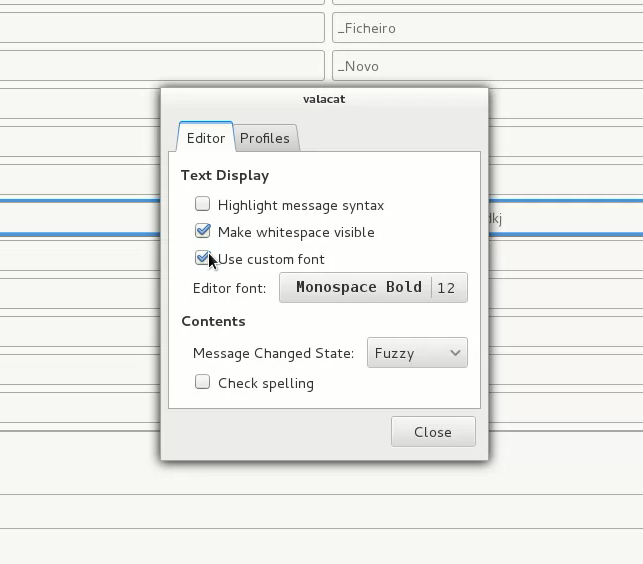
\includegraphics[width=0.7\textwidth]{img/gsoc1_it5_prefs.png}
    \caption{Diálogo de preferencias.}
    \label{fig:gsoc1_it5_prefs}
\end{figure}

Na Figura~\ref{fig:gsoc1_it5_prefs} pódese ver o aspecto deste dialogo.

\subsubsection{Mellorar a calidade do código e documentación}
Fixose unha revisión completa do código para manter un mesmo estilo ao largo de todo o código. Ademais actualizaronse os diagramas UML creados na primeira iteración.

\subsubsection{Reportes e Feedback}
Escibiuse un\footnote{\href{}{}} reporte

\subsubsection{Tarefas e seguimento}

\begin {itemize}
  \item Deseño e implementación das preferencias.
  \item Correxir Clase ficheiro.
  \item Correxir errores de estilos no código.
  \item Actualizar diagramas UML.
  \item Escribir reportes.
\end {itemize}

Planificaronse un total de  horas para a realización destas tarefas.

\subsection{Estado ao fin do GSoC 2013}
O finalizar esta iteración o mentor do GSoC avalía correctamente o proxecto presentado polo que o programa é completado con éxito. O programa entregado ten entre outras moitas as seguintes características:

\begin{itemize}
  \item Posibilidade de abrir ficheiros po.
  \item Navegación a través do documento.
  \item Posibilidade de buscar.
  \item Editor con resaltado de sintaxe e de espacios en branco.
  \item Preferencias.
\end{itemize}

Pero tamén presenta algúns fallos:

\begin{itemize}
  \item Lentitude ao cargar ficheiros moi grandes.
  \item Fallo ao gardar un ficheiro.
  \item O aspecto da interface non é satisfactorio.
  \item Problemas ao buscar.
\end{itemize}

Intentamos durante o curso seguinte nos tempos libres arreglar estos fallos.

\section{Primeiro cuatrimestre curso 2013/2014}

Durante este periodo intetouse continuar o proxecto durante o tempo libre polo que estas iteracións son maís longas no tempo xa que tráballase un menor número de horas. Distinguimos dúas iteracións que corresponden a dous momentos durante o curso na que a carga de traballo permitiume seguir co proxecto.

\subsection{Primeira iteración: cambios na interface}
A primeira iteración comprende os últimos días de septembro e o mes de octubro. Durante este tempo faise un rediseño da interface gráfica e implementanse as pistas e os comprobadores.

\subsubsection{Interface Gráfica}
Decidimos facer un re-deseño da interface para intentar conseguir un mellor resultado. Para facer esto empregamos os deseños iniciais que se asemellan máis o aspecto da aplicación Virtaal.

Xa tiñamos feitos os widgets de edición e a lista de mensaxes polo que facer o novo deseño consiste en misturar os dous conceptos. Na Figura~\ref{fig:curso2014_it1_ui} podese ver o resultado. Desta forma se facemos click nun dos mensaxes da lista este expandese e permitenos editar o contido.

\begin{figure}[h!]
    \centering
    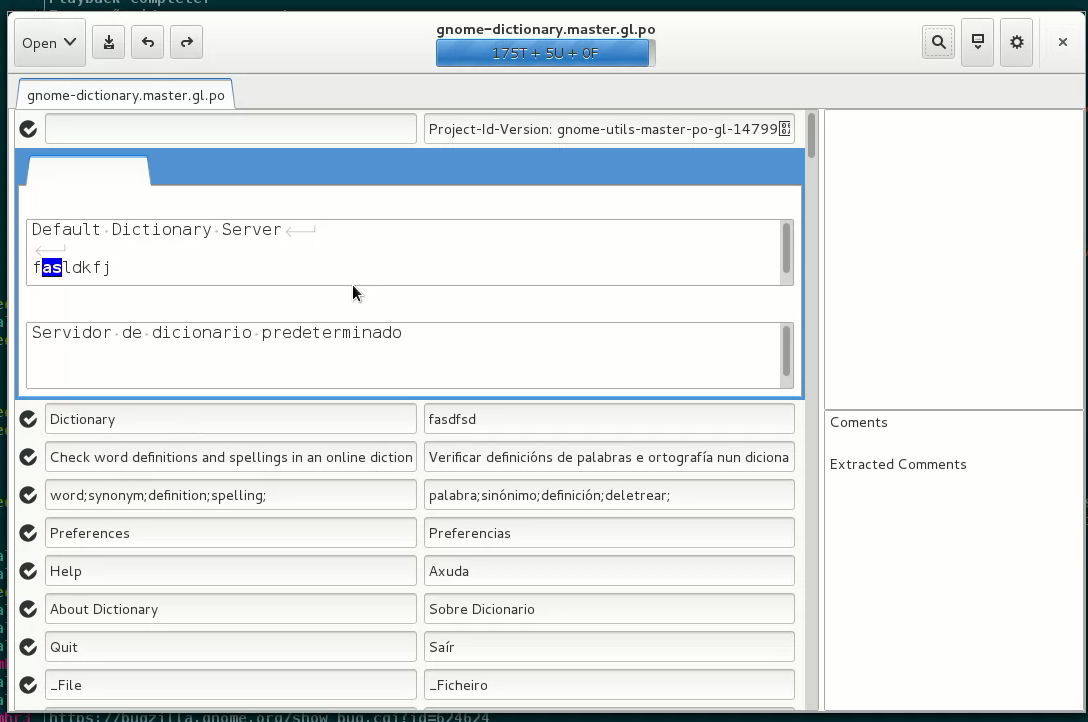
\includegraphics[width=0.8\textwidth]{img/curso2014_it1_ui.png} 
    \caption{Rediseño da interface}
    \label{fig:curso2014_it1_ui}
\end{figure}

Ademais deixamos de usar a biblioteca GDL xa que en conversacións a través de IRC chegouse a conclusión de que se o usuario tiña que usar esta biblioteca para modificar a interface isto é por que a interface está mal deseñada.


\subsubsection{Pistas e Comprobadores}
Como xa comentamos as pistas (\emph{hints}) son posibles traducións para unha cadea determinada. Nesta iteración creamos tanto o panel da interface que permite ver estas pistas como a clase que lle provee as pistas a dita interface. Por último creamos un mock para poder seguir traballando.

En canto aos comprobadores (\emph{checkers}), estos son os elementos do programa que aportan os consellos da mesma forma que cas pistas, implementamos a clase comprobador e crearmos un mock de nome \emph{DemoChecker}.

\subsubsection{Presentación GUADEC Hispana 2013 (Madrid)}

A GUADEC Hispana é unha reunión de usuarios e desarrolladores que falan castelán e que sirve tamén para a reunión anual (como obliga a lei) da organización GNOME Hispano. Ademais desta reunión fanse charlas sobre GNOME e outros temas relacionados.

\begin{figure}[h!]
    \centering
    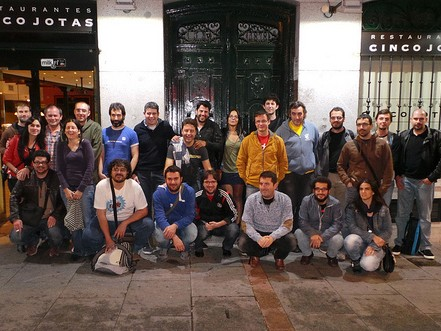
\includegraphics[width=0.495\textwidth]{img/guadec_es_2013_1.jpg}
    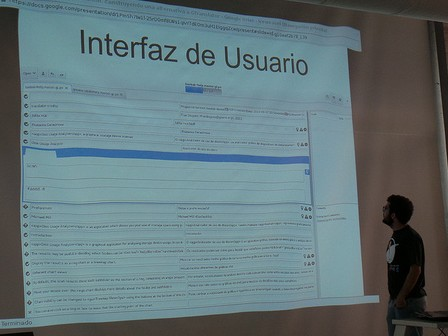
\includegraphics[width=0.495\textwidth]{img/guadec_es_2013_2.jpg} 
    \caption{GUADEC Hispana 2013 (Madrid)}
    \label{fig:guadec2012}
\end{figure}

Entre esas charlas deuse unha sobre o programa que se realiza neste proxecto na cal os asistentes amosaron o seu interes por que se seguira desenrolando.

\subsubsection{Reportes e feedback}
Escribiuse un reporte\footnote{\href{http://aquelando.info/changing-the-tool-ui/}{Changing the tool UI}} mais ninguén escribiu ningún comentario. Non obstante durante a GUADEC-es houbo xente que se interesou polo programa.

\subsubsection{Tarefas e seguimento}

As tarefas realizadas durante esta iteración foron as seguintes:

\begin{itemize}
  \item Implementar Pistas e Proveedor de Pistas.
  \item Implementar Comprobador.
  \item Interface de Usuario.
    \begin{itemize}
      \item Eliminar biblioteca GDL.
      \item Engadir widget de Pistas.
      \item Mezclar lista de mensaxes con editor de mensaxes.
    \end{itemize}
\end{itemize}

Para estas tarefas planificaronse 50 horas que se completaron con éxito.

\subsection{Segunda iteración: Refactorizar navegadores e melloras na interface}
Esta iteración sucede durante o mes de novembro e os primeiros días de decembro.

\subsubsection{Refactorización dos navegadores}

\subsubsection{Cambio de nome}
Como nos pediron dende a GNOME Foundation, cambiamos o aplicativo de nome. O nome escollido o final é GNOMECAT. Eleximos este nome pois pensamos que o programa non é un traductor xa que non traduce el solo e isto pode levar a enganos. Para facer este cambio modificamos tanto o código como os ficheiros de configuración.

\subsubsection{Interface de usuario}

\subsubsection{Reportes e Feedback}
Escribese un\footnote{\href{http://aquelando.info/welcome-gnomecat/}{Welcome GnomeCAT}} contando os últimos avances do aplicativo e o cambio de nome. Recibimos un comentario dicindo que GNOME escribese con letras maiusculas polo que temos que correxir o programa. Outra xente interesase polo significado de CAT.

\subsubsection{Tarefas e seguimento}

\begin{itemize}
  \item Cambiar nome do aplicativo.
  \item Refactorizar navegadores.
  \item Interface de usuario.
\end{itemize}

\subsection{Presentación para o GSoC 2014}
Debido a evidente falta de tempo para completar o programa durante os ratos libres decidese presentar o programa de novo o proxecto Google Summer of Code. Falase coa cordinadora dos programas de iniciación en GNOME para saber se isto é posible e repondenos afirmativamente. Como mentor falamos co \emph{maintainer} de GTranslator que nos di que non ten ningún problema en facer de mentor. Presentamos o proxecto e este sale aceptado.

\section{Google Summer of Code 2014}
%GSoC 2014 -> 19 de Maio - 11 Agosto -> 15 - 1 (guadec) - 1 (traballo r) -> 325h


\subsection{Primeira iteración: Rediseño UI}
 %19 May - 1 June

I have one exam on 22nd of May so I’m not going to be able to do something until the next day. I will discuss the open menu and settings panel redesign with the GNOME Design team and I will start to implement this changes 
%(#11, #19, #21). 

\subsection{Segunda Iteración: Rediseño UI}
%2 June - 15 June

I will finish this changes and I will implement file tab and project tab discussing the design previously with the Design team.  Some other UI related issues will be treated also this first month. . The final aspect of the application should be finished when this period ends.
%(#3, #9, #24) (#12, #14, #15, #23)

\subsection{Terceira Iteración: Buscas}
%16 June - 29 June

I will implement project search and I’m going to fix the failures related to file searches.. This increment deliverables are the search feature fully implemented.
% (#17, #23)

\subsection{Cuarta Iteración: Bindings GetText-PO e carga de ficheiros grandes.} %30 June - 13 July

I’m going to fix and improve the gettext-po bindings. The program works really slow with big files and this should be fixed someway. During this increment we should improve the speed load of the application and we should be able to open big f

\subsection{Quinta Iteración: Plugins e atallos de teclado} %14 July - 27 July

Implement plugins engine and keyboard shortcuts. And write some basic plugins like a simple translation memory. This period deliverable is the possibility of extend the application features using plugins.
% #4 e #5

\paragraph{Presentación GUADEC 2014 (Strasbourg)}

\begin{figure}[h!]
    \centering
    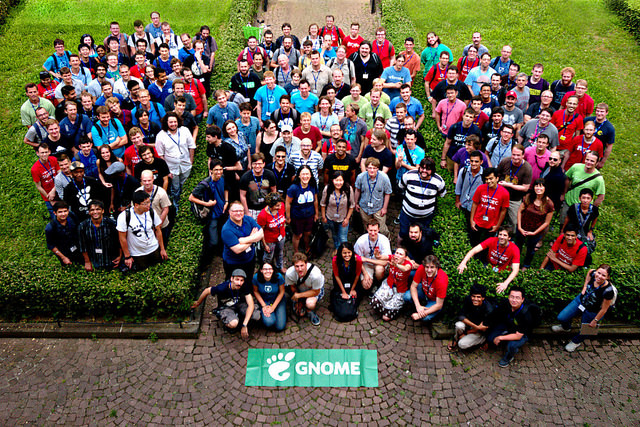
\includegraphics[width=0.999\textwidth]{img/guadec_2014.jpg}
    \caption{GUADEC 2014 (Strasbourg)}
    \label{fig:guadec2012}
\end{figure}


\subsection{Sexta Iteración: Detalles finais e escribir documentación} %28 July - 10 Agosto

Polish the final details and write documentation. By the end of this increment the application should be finished.
% #13 e  #25


\subsection{Estado ao fin do GSoC 2014}

\section{Segundo cuatrimestre 2014/2015}

        \chapter[Análise de Requisitos]{Análise de Requisitos globais}

Neste capítulo explicaremos o proceso de análise de requisitos levado a cabo para a construción da ferramenta.

\section{Consultas cos tradutores}
Para facer unha nova ferramenta de asistencia á tradución consultamos os usuarios principais da ferramenta. Para iso enviamos correos a unhas cantas listas de correo de tradutores de diferentes proxectos de software libre como os seguintes:

\paragraph{GNOME} Dentro do proxecto GNOME hai un grupo específico para a internacionalización dos programas da plataforma. Existen listas de correo para cada linguaxe e unha a nivel internacional. En concreto as listas ás que enviamos un correo preguntando por ideas para o novo programa, foron a lista \emph{internacional}, a lista de tradutores ó \emph{galego} e a lista de tradutores ó \emph{castelán}.

\paragraph{Proxecto Trasno} É unha comunidade de tradutores de proxectos de software libre ao Galego. Serve de punto de encontro para os tradutores galegos e realiza periodicamente reunións para a discusión da terminoloxía a usar e a presentación de novas ferramentas.

\paragraph{OpenSuse e Fedora} Estas dúas distribucións de Linux contan cos seus respectivos equipos de tradutores. Aínda que a maior parte dos programas destas distribucións son traducidos por outros proxectos, como pasa no caso do entorno de escritorio GNOME, si que hai partes do sistema que necesitan ser traducidas polos propios tradutores de cada distribución.

\paragraph{OpenOffice e LibreOffice} Tanto OpenOffice como o seu \emph{fork}, LibreOffice, contan con equipos internacionalización aos que se lles consultou para recoller ideas para o novo programa.

\paragraph{Mozilla} O proxecto Mozilla, autores do navegador Firefox e do xestor de correo electrónico Thunderbird, conta cun equipo de tradutores propio. Neste caso non usan ficheiros de tipo Gettext PO, senón tamén ficheiros XML.

Case en todos os correos enviados houbo xente que respondeu dando ideas sobre o que lles gustaría que se incorporase ó novo programa. Na seguinte sección podemos ver a maioría destas utilidades explicadas.

\subsection{Resumo das peticións}
	\paragraph{Abrir e gardar ficheiros en diferentes formatos.} O programa debería permitir abrir outros formatos de ficheiros aparte do formato Gettext po. Esta petición foi feita sobre todo por membros de equipos de tradutores que non son de GNOME. Existe unha biblioteca de nome \emph{translate-toolkit} que facilita a conversión entre formatos.

	\paragraph{Xestión de cabeceiras} Que o programa modifique automaticamente as cabeceiras con metainformación que tanto o formato Gettext PO como outros tipos de formatos teñen.

	\paragraph{Perfiles de usuarios} Permitir ter diversos perfiles de usuarios para diferentes proxectos de tradución ou para diferentes linguaxes.

	\paragraph{Vista de proxecto} Os tradutores consideran moi interesante agrupar os ficheiros relacionados en proxectos e poder ter estatísticas de proxectos.

	\paragraph{Buscar e buscar e reemplazar} O programa debe permitir buscar e reemplazar palabras dentro do documento.

	\paragraph{Dividir/Misturar ficheiros} Os tradutores consideran que é interesante que en ficheiros grandes exista a posibilidade de dividir e volver a unir ficheiros de tradución para que así sexa posible que máis dunha persoa traballe no mesmo ficheiro a vez.

	\paragraph{Medidas Económicas} É interesante incorporar unha ferramenta que permita calcular o custe da tradución efectuada por un tradutor. Istó é especialmente útil cando falamos de tradutores profesionais e non amateur.

	\paragraph{Resaltado da síntaxe} O programa debe resaltar aqueles elementos da cadea que non son traducibles e pertencen o dominio das linguaxes de programación. Por exemplo na seguinte cadea \lstinline[language=C]{"Temos %i coches."} o elemento \lstinline[language=C]{%i} debería estar resaltado xa que so parte do formatado da cadea por parte do programa.

	\paragraph{Comunicación con servidor web} Os tradutores consideran a posibilidade de que o programa permita certa comunicación con xestores de traducións en internet. No caso de GNOME o programa Damned Lies xestiona os ficheiros .po para todos os programas de GNOME e os tradutores deben baixar e subir os ficheiros dende esa plataforma.

	\paragraph{Navegación dentro do documento} A posibilidade de navegar a través das cadeas. Engadir a posibilidade de ir á seguinte cadea traducida, sen traducir ou con unha tradución difusa.

	\paragraph{Memoria de tradución} Engadir unha memoria de tradución que permita exportar e importar ficheiros en diferentes formatos. Ter varias memorias  de tradución con prioridade entre elas, engadir a posibilidade de editar a memoria de tradución e acceder a diversos servidores que xestionan memorias de tradución online como poden ser Trobador, amaGama, Open-tran ou Transvision.

	\paragraph{Glosario} Engadir a posibilidade de consultar a tradución de termos contra ficheiros unha base de datos local ou contra un servidor de glosario como pode ser Terminator.

	\paragraph{Busca de termos} Que o programa permita a busca nun dicionario tanto local como en internet. Cítanse dicionarios en internet como o que proporciona Wikipedia ou a Universidade de Santiago de Compostela para o galego.

	\paragraph{Previsualización das traducións} Moitas das interfaces que se fan actualmente empregan ferramentas de cuarta xeración que permitirían xerar a interface coas traducións. No caso de GNOME, Glade é o programa que permite a creación de interfaces e xa existe unha ferramenta online que permite a previsualización de traducións de nome Deckard. O que se pide é que o programa incorpore esa posibilidade dende a súa interface.

	\paragraph{Programa controlable totalmente a través do teclado} O programa en xeral, pero sobre todo a interface de edición de ficheiros, debe ser manexable totalmente a través do teclado para mellorar a produtividade dos tradutores. Os tradutores piden tamén a posibilidade de que se permita personalizar os atallos de teclado.

	\paragraph{Tradución doutras linguaxes} Hai linguas como o galego e o portugués que se parecen moito polo que, as veces, resulta moi útil poder, en vez de partir de cero, coller unha tradución dun idioma semellante e editala.

	\paragraph{Comprobacións} Os tradutores resaltaron a utilidade de que a ferramenta comprobe certos parámetros para comprobar a calidade da tradución. Entre outros:
		\begin{itemize}
			\item \textbf{Ortografía e Gramática.} O programa avisará se a cadea traducida ten erros tanto ortográficos como gramaticais.
			\item \textbf{Coherencia terminolóxica.} O programa avisará ó usuario cando este empregue unha tradución dun termo diferente o que se vén empregando no resto do ficheiro.
			\item \textbf{Etiquetado XML e marcas de formato.} O programa avisará ó usuario se faltan ou están mal escritos as diferentes etiquetas XML ou marcas de formato.
		\end{itemize}

	\paragraph{Multiplataforma} A aplicación debe estar dispoñible para varios sistemas operativos (BSD, Windows, MAC OS, etc.).

	\paragraph{Tradución automática} O aplicativo debe incorporar mecanismos de tradución automática empregando ferramentas como Google Translator, Bing Translator, Opentrad ou Apertium.

	\paragraph{Estatísticas} Débese amosar estatísticas tanto a nivel de ficheiro como de proxecto do número de cadeas ou palabras traducidas, sen traducir ou difusas.

\section{Análise doutros aplicativos do mercado}
Para facer o novo produto software para a tradución tamén consultamos outras ferramentas similares existentes no mercado para intentar imitar as súas vantaxes e evitar as súas deficiencias. O resultado desta análise pódese consultar na Sección~\ref{sec:ferramentascat}.

\section{Requisitos do aplicativo}
Con toda a información obtida realizamos unha lista de casos de uso que debe cumprir o programa.

\begin{itemize}
  \item \textbf{Abrir ficheiro.} O programa debe ser capaz de abrir ficheiros PO pero tamén ter un deseño extensible que permita abrir outros formatos.
  \item \textbf{Gardar ficheiro.} Debemos poder gardar ficheiros PO pero tamén ter un deseño extensible que permite gardar noutros formatos.
  \item \textbf{Amosar ficheiro.} Debemos amosar o contido dos ficheiros e dicir, as cadeas e as estatísticas deste ficheiro.
  \item \textbf{Editar ficheiro.} Debemos permitir editar o contido dos ficheiros.
  \item \textbf{Buscar cadeas.} A aplicación permitirá buscar entre as cadeas do ficheiro.
  \item \textbf{Navegar polas cadeas.} Permitiremos navegar polas cadeas do ficheiro podendo avanzar entre as cadeas traducidas, sen traducir, etc.
  \item \textbf{Xestionar perfiles.} Permitiremos xestionar diferentes perfiles para os tradutores.
  \item \textbf{Obter pistas.} Amosaremos ao usuario pistas que lle indiquen que está a facer algo mal.
  \item \textbf{Obter suxerencias.} Debemos amosar ao tradutor diferentes alternativas de traducións.
\end{itemize}

Na figura~\ref{fig:casosdeuso} podemos ver o Diagrama UML de casos de uso para este programa.

\begin{figure}[h!]
    \centering
    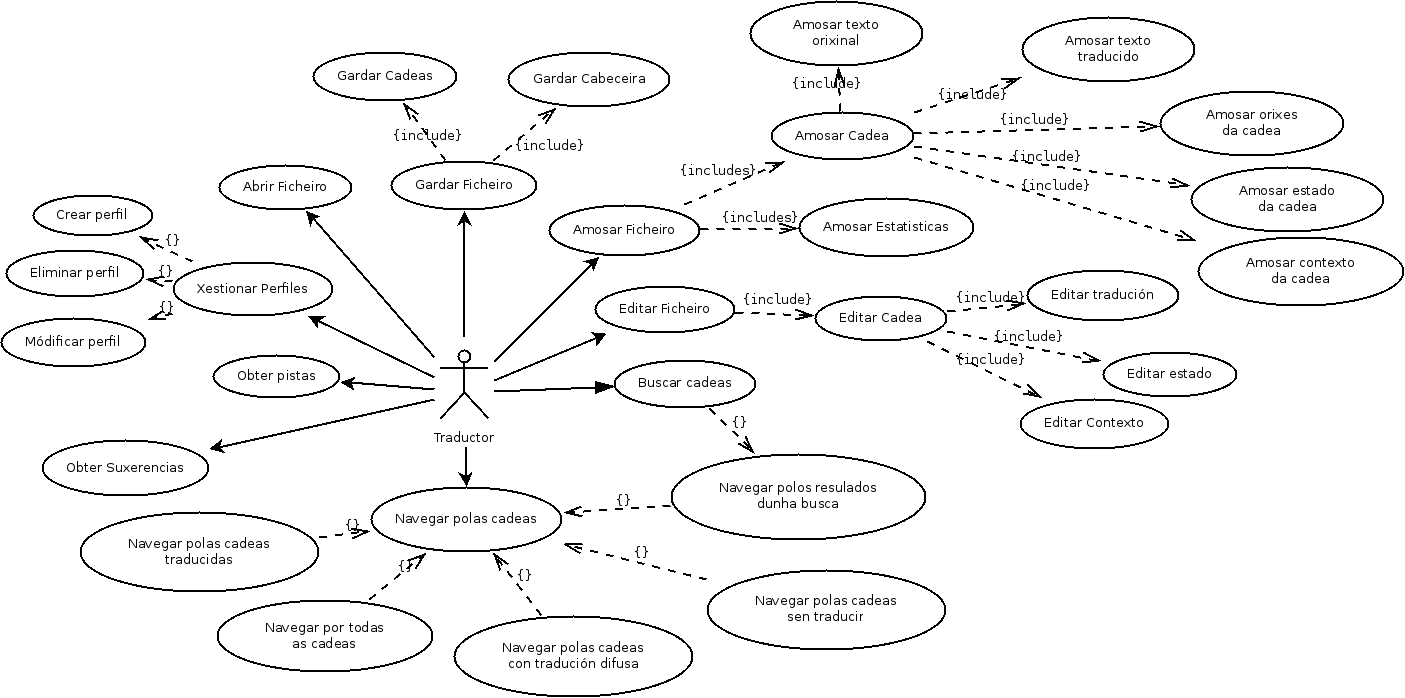
\includegraphics[width=0.9\textheight,angle=90]{img/casosdeuso.png}
    \caption{Diagrama UML de casos de uso do aplicativo}
    \label{fig:casosdeuso}
\end{figure}

%
% FIN DEL CAPÍTULO
%

        \chapter{Deseño e Implementación}

Neste capítulo veremos detalles do deseño e implementación de diferentes partes do programa.

\section{Módulo de Ficheiros}

O módulo de xestión de ficheiros é un do máis importantes e complexos de todo o programa, o cal é lóxico tendo en conta que o programa é un editor de ficheiros.

En canto ao deseño, ó principal obxectivo é a estensibilidade do mesmo pois, aínda que o programa está centrado na edición de ficheiros PO e son estes os únicos soportados na actualidade, preténdese que o programa sexa capaz de soportar varios tipos de ficheiros nun futuro. Na figura~\ref{fig:dia_class:files} pódese ver o diagrama de clases deste módulo.

\subsection{Implementación Xenérica}
A implementación da clase \lstinline{File} contén propiedades para conseguir información sobre o nome e \emph{path} onde está dito ficheiro, ademais garda estatísticas sobre o número de mensaxes traducidos, sen traducir ou con tradución difusa. Estas estatísticas actualízanse cada vez que se engade ou elimina unha cadea ou cada vez que esta se modifica. Tamén contén un valor booleano que permite saber se o ficheiro foi modificado. Aparte de métodos para engadir e eliminar cadeas, e para conseguir e modificar os metadatos do ficheiro esta clase ten un método para gardar e recuperar o ficheiro. O método para gardar~(\lstinline{save}) emprega o patrón \emph{Template Method}\cite{book:gang4pat} o cal nos permíte actualizar o estado do ficheiro a non modificado.

Un ficheiro contén instancias de mensaxes~(\lstinline{Message}). As mensaxes teñen como propiedades un estado, orixes, e consellos. A API prové métodos para conseguir e modificar tanto as cadeas orixinais como as traducións, na súa forma en singular ou nalgunha das formas plurais. A implementación do método para modificar unha tradución tamén emprega o patrón Template Method para actualizar o estado da mensaxe. Esta clase tamén ten métodos para engadir e eliminar consellos e para obter o contexto da mensaxe.

\begin{figure}[h!]
    \centering
    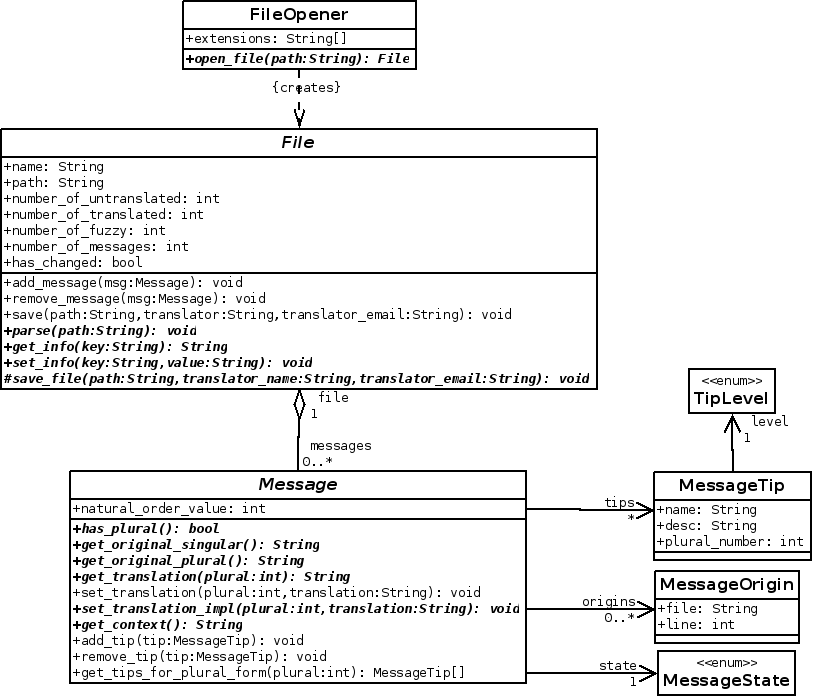
\includegraphics[width=\textwidth]{img/genericfile.png}
    \caption{Diagrama de Clases do módulo ficheiros}
    \label{fig:dia_class:files}
\end{figure}

Ademais a clase \lstinline{FileOpener} recolle un método para crear ficheiros e un conxunto de extensións que se poden abrir con este FileOpener.

\subsubsection{Consellos (Tips)}
Os consellos son a solución que damos para aportar información ao usuario sobre a tradución que está a realizar. Algunhas das cousas que poden axudar a indicar esta característica son se a tradución está a ser demasiado longa, se hai algunha palabra que está mal escrita na tradución ou se non emprega a terminoloxía adecuada.

Cada consello ten un nome que debe ser xenérico a cada clase de consello, unha descrición que ten que explicar o problema con detalle, un nivel que indica a gravidade do consello e unha referencia a forma plural a que corresponde dito consello. Ademais, pode conter unha ou máis referencias á localización exacta do problema que permitirá destacala na interface gráfica.

A creación de consellos farase ó modificarse unha cadea e farase a través de plugins.

\subsubsection{Pistas (Hints)}
As pistas amosaranlle ó usuario posibles traducións ou aproximacións ás traducións. Estas pistas poden ser obtidas de memorias de traducións, de traducións do mesmo ficheiro noutra linguaxe, ou da tradución directa, por exemplo.

Cada instancia dunha pista~(\lstinline{Hint}) contén a tradución suxerida, unha cadea que identifica a orixe de dita pista e un valor que indica a precisión de dita suxerencia.

De igual forma que no caso dos consellos a creación de pistas correrá ó cargo de plugins creados a tal propósito. Neste caso actualizaranse as pistas de cada mensaxe ao seleccionalo mesmo na interface.

\subsection{Ficheiro PO}
A implementación específica para ficheiros PO (Figura~\ref{fig:dia_class:pofile}) estende as clases \lstinline{File}, \lstinline{FileOpener} e \lstinline{Message} abstractas para implementar os métodos e permitir empregar ficheiros PO.

Para a análise e a actualización dos ficheiros PO empregaremos a biblioteca gettext-po. No momento no que se iniciou a implementación deste módulo, non existía implementación desta librería en Vala polo que tivemos que crear uns \emph{bindings} para poder empregala.

Tanto a clase PoFile como a clase PoMessage delegan a maior parte dos seus métodos nas instancias das clases dos bindings da biblioteca GettextPo File e Message respectivamente. Desta forma faise un claro uso do patrón \emph{Adapter}\cite{book:gang4pat}.

\begin{figure}[h!]
    \centering
    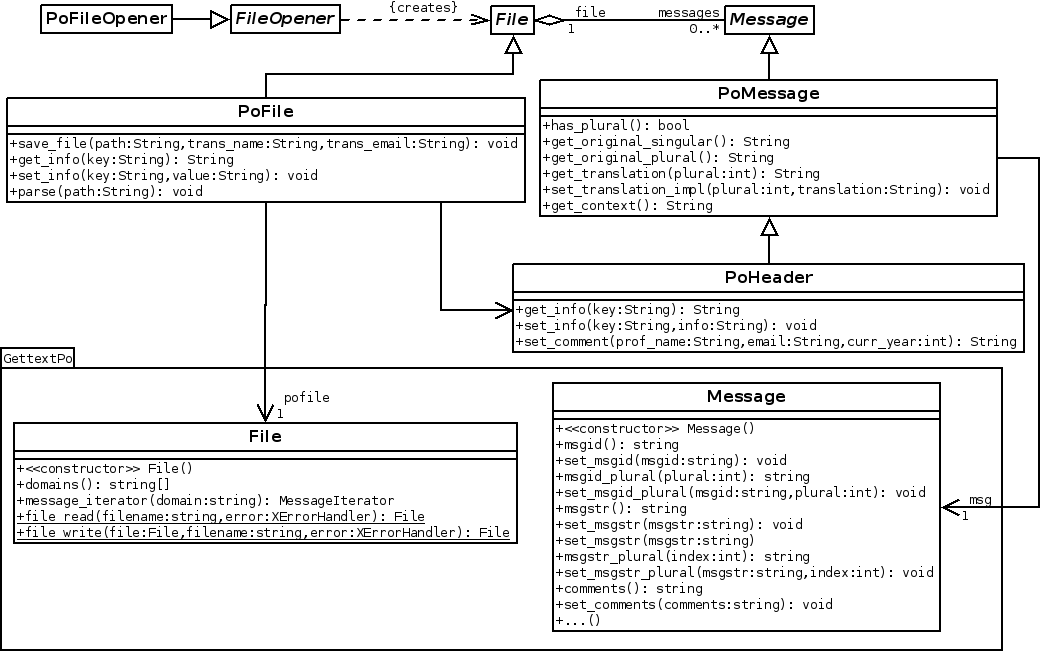
\includegraphics[width=\textwidth]{img/pofile.png}
    \caption{Diagrama de Clases do ficheiro PO}
    \label{fig:dia_class:pofile}
\end{figure}

De forma adicional, a clase PoFile contén unha instancia da clase PoHeader. Esta clase que estende a PoMessage ten os metadatos que se atopan nos ficheiros PO na tradución da cadea baleira. Ademais, esta, dipón de métodos para obter e modificar metadatos e para actualizar os datos dos autores das traducións de dito ficheiro. A clase PoFile delega nesta clase á hora de conseguir e modificar metadatos e tamén cando garda un ficheiro.

A clase \lstinline{PoFileOpener} só é capaz de abrir ficheiros con estensión PO e simplemente emprega o método parse da clase ficheiro para crear unha nova instancia.

\subsubsection{Implementación dos bindings}
Como xa mencionamos vímonos na obriga de crear nós os bindings para a biblioteca gettext-po. Vala é unha linguaxe deseñada para permitir o fácil acceso a outras bibliotecas escritas en C, especialmente se se trata de bibliotecas baseadas en GObject. Despois de todo Vala emprega C como linguaxe intermedio. A biblioteca gettext-po non é unha biblioteca baseada en GObject polo que a creación destes bindings é un pouco máis complicado.

Para poder empregar unha biblioteca escrita en C no noso programa escrito en Vala só temos que crear un ficheiro con extensión VAPI que conteña en sintaxe Vala as clases da biblioteca engadindo unhas etiquetas que permitan a súa tradución ó código C correcto. No Fragmento de código~\ref{lst:bindingsgettext} podemos ver parte dos bindings creados para a biblioteca gettextpo.

\lstset{language=[sharp]C}
\begin{lstlisting}[label=lst:bindingsgettext,caption=Bindings da biblioteca GettextPo]
[CCode (cprefix = "Po", lower_case_cprefix = "po_")]
namespace GettextPo {

    [CCode(cheader_filename = "gettext-po.h", cname="struct po_file", free_function="po_file_free")]
    [Compact]
    public class File {

        [CCode (CCode = "po_file_create")]
        public File();

        [CCode (array_length = false, array_null_terminated = true, cname="po_file_domains")]
        public unowned string[] domains ();

        [CCode (cname="po_file_write")]
        public static unowned GettextPo.File file_write (GettextPo.File file,
                            string filename,
                            XErrorHandler handler);
        [...]
    }

    [CCode(cheader_filename = "gettext-po.h", cname="struct po_message")]
    [Compact]
    public class Message  {

        [CCode (cname="po_message_create")]
        public Message();
        public unowned string msgid ();
        public unowned string? msgid_plural ();
        [...]
\end{lstlisting}

Como podemos ver, o traballo practicamente limítase a establecer o parámetro \lstinline{cname} en cada clase e método. Hai que ter en conta que non sempre é necesario especificar este parámetro pois as bibliotecas empregan case sempre unhas normas de nomeado que fan que usen primeiro o nome da biblioteca, despois o nome da clase e logo o nome do método separado por barras baixas. Desta forma no método da biblioteca \lstinline{po_message_msgid()}, \emph{po\_} corresponde o nome da biblioteca, \emph{message\_} ao nome da clase e \emph{msgid} ao nome do método. Os bingings de Vala empregan estas normas para nomear os métodos polo que, en ocasións, non é necesario especificar o parámetro \lstinline{cname}. Isto sucede, como se pode ver no Fragmento de código~\ref{lst:bindingsgettext}, no caso da clase Mensaxe (\lstinline{Message}).

Ademais, é necesario especificar o nome do ficheiro cabeceira que se emprega e no caso de que o tipo de retorno sexa un array temos que especificar máis parámetros, como acontece no método \lstinline{domains()} da clase File. Por último, é importe especificar a pertenza de cada valor e os métodos correctos para liberar as instancias, desta forma evitaremos que haxa perdas de memoria e fallos de segmentación.

\section{Módulo de Linguaxes}
O módulo de linguaxes xestiona os linguaxes e formas plurais existentes. Contén dúas clases, a clase \lstinline{Language} e a clase \lstinline{PluralForm}. Estas dúas clases provén un método estático para obter as instancias existentes. Estas instancias créanse a primeira vez que se carga a clase consultando unhas bases de datos que consisten nuns ficheiros JSON\footnote{\href{http://gl.wikipedia.org/wiki/JSON}{JSON}}.

\begin{figure}[h!]
    \centering
    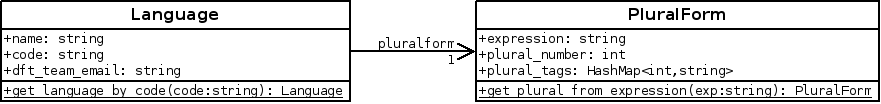
\includegraphics[width=\textwidth]{img/languages.png}
    \caption{Diagrama de Clases do módulo de Linguaxes}
    \label{fig:dia_class:languages}
\end{figure}

Como podemos ver na Figura~\ref{fig:dia_class:languages}, en cada instancia dunha linguaxe contén o nome da linguaxe, o seu código empregando a norma ISO 639-1, a súa forma plural e o email do equipo de tradución por defecto. Engadimos o idioma do equipo de tradución por defecto para autocompletar este campo no perfil do usuario. No Fragmento de Código~\ref{lst:languages} podemos ver un fragmento do ficheiro JSON contendo as linguaxes.

\begin{lstlisting}[label=lst:languages,caption=Fragmento da Base de Datos de Linguaxes]
  {
    "languages" : [
      [...]
      {
        "code" : "es",
        "name" : "Spanish; Castilian",
        "pluralform" : "nplurals=2; plural=(n != 1);",
        "default-team-email": "gnome-es-list@gnome.org"
      },
      [...]
    ]
  }
\end{lstlisting}

En canto á clase \lstinline{PluralForm}, esta clase inclúe o número de plurais, a expresión desa forma plural e un conxunto de etiquetas. Estas etiquetas pretenden facilitar ó usuario a identificación de que número corresponde a cada forma plural. No Fragmento de Código~\ref{lst:plurals} pódemos ver unha parte da base de datos de formas plurais.

\begin{lstlisting}[label=lst:plurals,caption=Fragmento da Base de Datos de Plurais]
  {
    "forms" : [
      {
        "expression" : "nplurals=2; plural=(n > 1);",
        "number_of_plurals" : 2,
        "tags" : [
          {
            "number" : 0,
            "tag" : "Equal to 0 or 1"
          },
          {
            "number" : 1,
            "tag" : "Greater than 1"
          }
        ]
      },
      [...]
    ]
  }
\end{lstlisting}

\section{Interface Gráfica}
A interface gráfica é unha das partes á que máis tempo lle dedicamos neste proxecto. O obxectivo dende o principio foi construír algo simple pero potente que permitira ó usuario editar os ficheiros PO de forma sinxela, pero que fose capaz de aportarlle moita información que lle axudase a facer a tradución.

\subsection{Evolución}
Durante a execución do proxecto probamos diferentes formas da interface gráfica ata chegar ó resultado actual. Estas versións pretenden imitar programas existenttes e obedecen xeralmente a conversacións con tradutores.

\subsubsection{Primeira Versión: moi semellante a GTranslator}
Para comezar a traballar, e tras amosar varios mockups nos reportes recibindo feedback sobre eles, decidimos facer unha interface de usuario moi parecida a de GTranslator. Esta interface inclúe bloques para a lista de mensaxes, editar ditos mensaxes e amosar o contexto. Estes bloques pódense mover por toda a interface e incluso separar da mesma xa que estamos empregando a biblioteca GNOME Docking Library. Na Figura~\ref{fig:ui:v1:general} podemos ver, o aspecto desta primeira versión da interface.

\begin{figure}[h!]
  \centering
    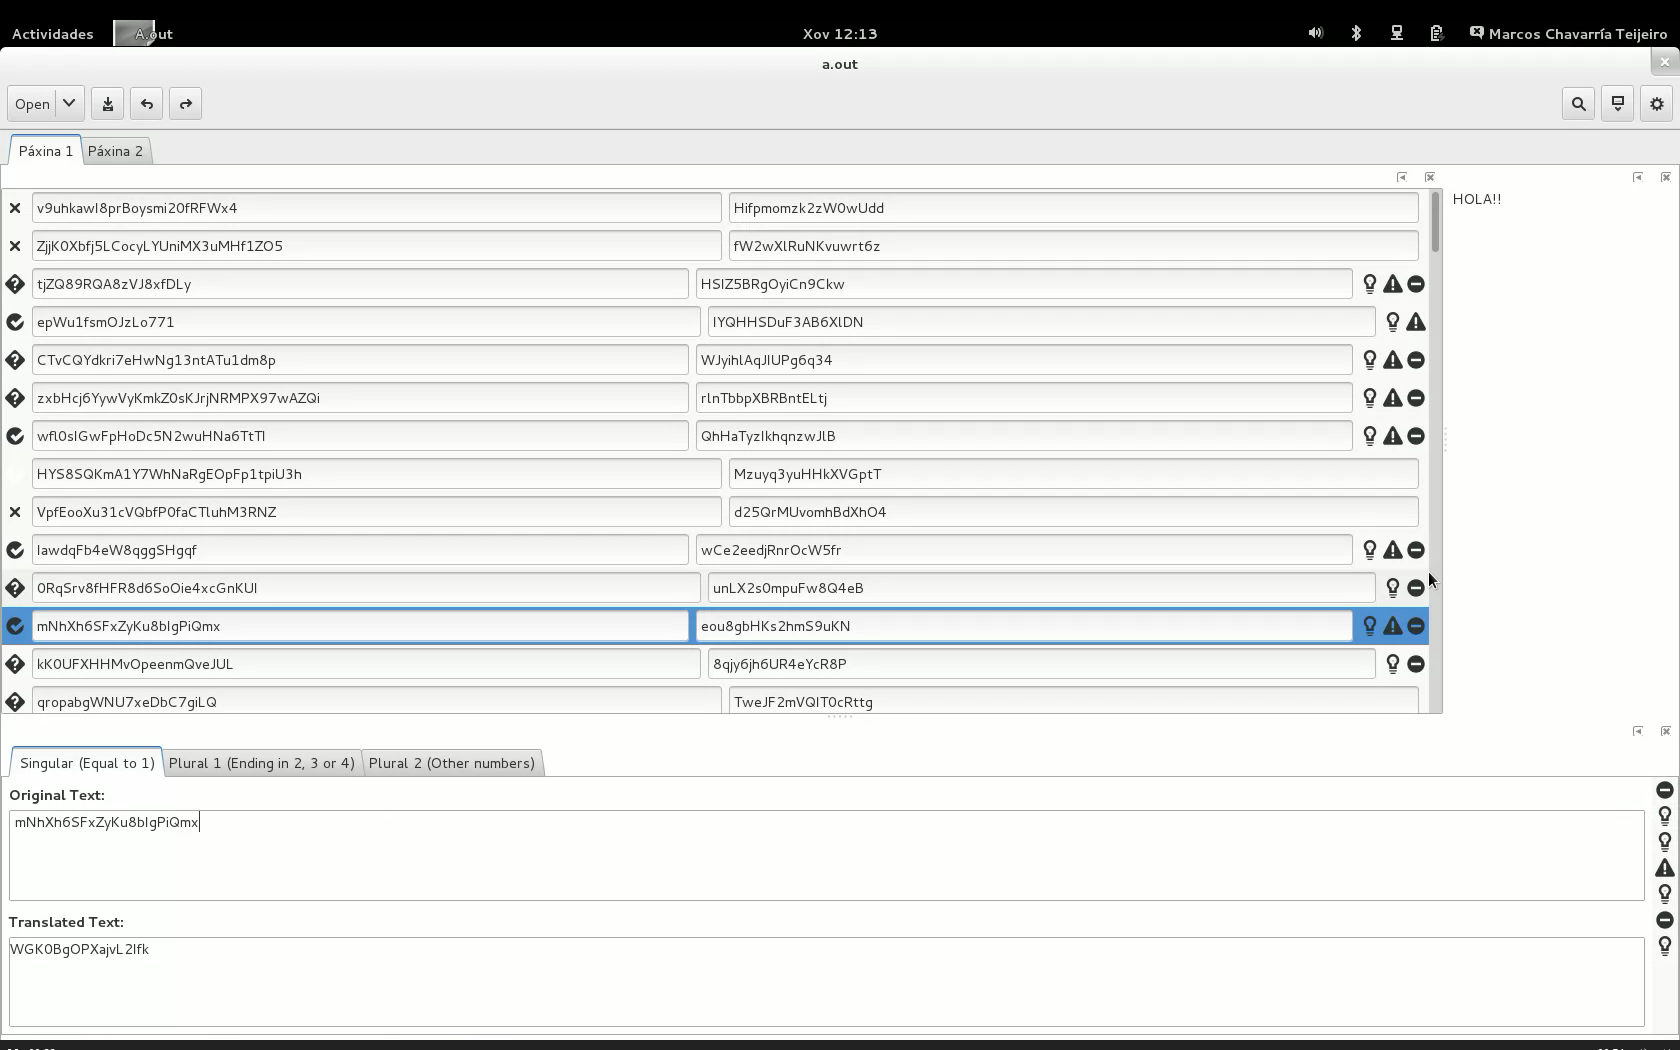
\includegraphics[width=\textwidth]{img/gsoc1_it2_ui.png}
    \caption{Primeira versión da interface de usuario}
    \label{fig:ui:v1:general}
\end{figure}

Como podemos ver a interface contén un barra de ferramentas que permite abrir ficheiros, gardalos, desfacer e refacer cambios, buscar no documento e ver as preferencias. Permite abrir diversos ficheiros en varias lapelas. En cada unha das lapelas podemos ver a lista de mensaxes e o widget de edición.

En cada mensaxe da lista, aparte das cadeas orixinal e traducida, podemos ver o estado da cadea e se está ten consellos (Tips) activos e de o nivel de estes. Por outro lado, no widget de edición podemos ver unha lapela por cada forma plural que podemos editar e unha lista vertical con iconas cos consellos. Ao pasar o rato polo consello veremos a súa descrición.

\begin{figure}[h!]
  \centering
  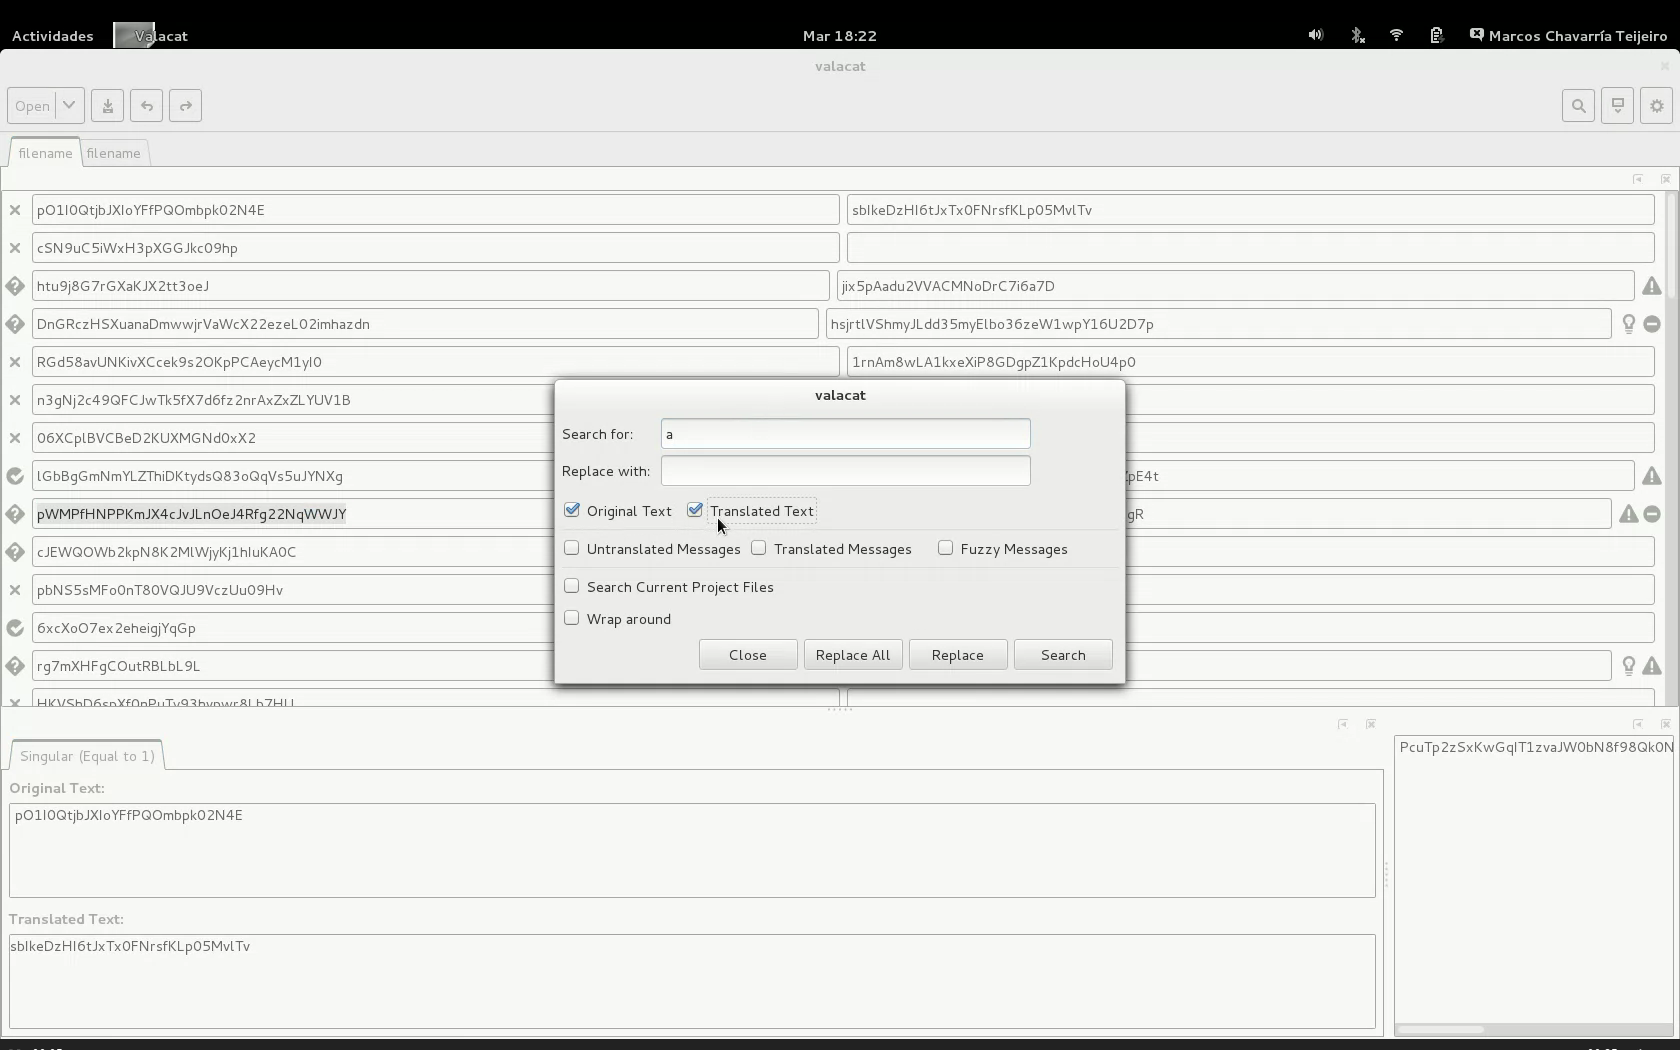
\includegraphics[width=0.4\textwidth]{img/gsoc1_it3_ui.png}
  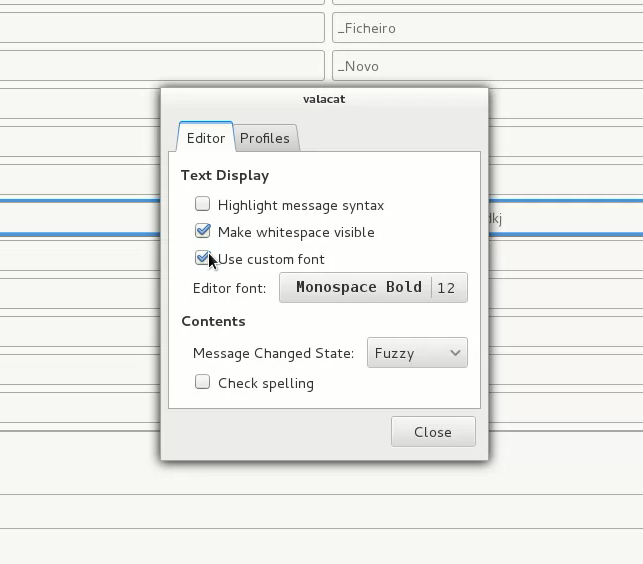
\includegraphics[width=0.4\textwidth]{img/gsoc1_it5_prefs.png}
  \caption{Diálogos da primeira versión da interface de usuario}
  \label{fig:ui:v1:dialogs}
\end{figure}

Como podemos ver na Figura~\ref{fig:ui:v1:dialogs} tanto á hora de xerar unha busca como para ver as preferencias, esta interface empregará uns diálogos non modais.

En conversacións en IRC con tradutores e anteriores mantedores de GTranslator chegamos á conclusión de que o uso de GNOME Docking Library era unha mala idea, pois significaba un erro de deseño xa que, se o usuario tiña que modificar o aspecto da interface, era debido a que o deseño non era correcto. Esta biblioteca, ademais, ten bastantes fallos polo que non era recomendable usala.

Ademais, durante a GUADEC, comentáronos da existencia dun widget moito mellor para xestionar a buscas, consistente nunha barra horizontal que se desplegaba cando a busca estaba activa.

Por outro lado, o resultado deste modelo de interface tampouco era demasiado satisfactorio polo que intentamos probar cunha versión máis próxima ó programa Virtaal.

\subsubsection{Segunda Versión: semellante a Virtaal}

Para lograr un aspecto máis parecido ó da aplicación Virtaal fusionamos o widget de edición e o widget de lista de cadeas.

A aplicación segue mantendo as lapelas que permiten abrir máis dun ficheiro ó mesmo tempo, pero eliminamos a posibilidade de personalizar a interface. En lugar diso crearemos unha interface con dúas columnas, na primeira teremos o widget para listar e editar as cadeas e na segunda un widget para ver o contexto e outro para ver as pistas.

Modificamos a barra de ferramentas que converteremos nun \lstinline{GTK.HeaderBar} que permite fusionar esta barra de ferramentas co marco da ventá. O uso de HeaderBars son un patrón de deseño recomendado por GNOME na súa Guía de Interfaces Humanas (\emph{HIG})\cite{website:gnomehig}. Na Figura~\ref{fig:ui:v2:general} podemos ver como quedou a nova inteface.

\begin{figure}[h!]
  \centering
    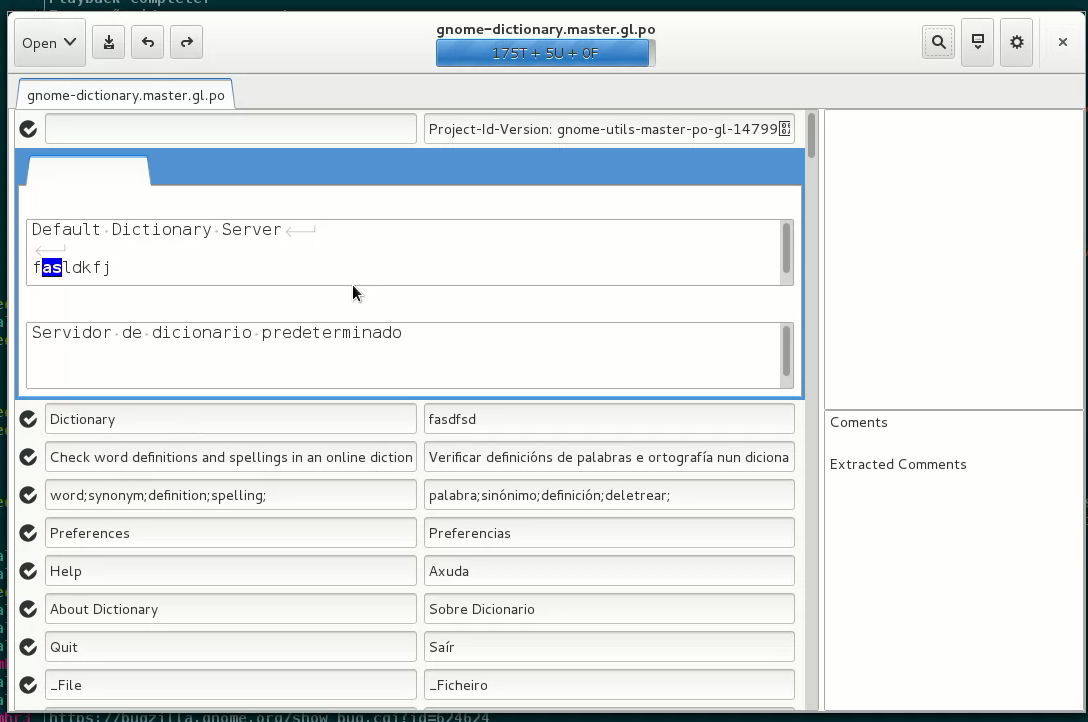
\includegraphics[width=\textwidth]{img/curso2014_it1_ui.png}
    \caption{Segunda versión da interface de usuario}
    \label{fig:ui:v2:general}
\end{figure}

Outro dos aspectos da interface no que se traballou foi na eliminación do diálogo de nova busca. Como se pode ver na Figura~\ref{fig:ui:v2:search}, ó activar a busca, desplégase unha barra horizontal que permite introducir termos para buscar.

\begin{figure}[h!]
  \centering
    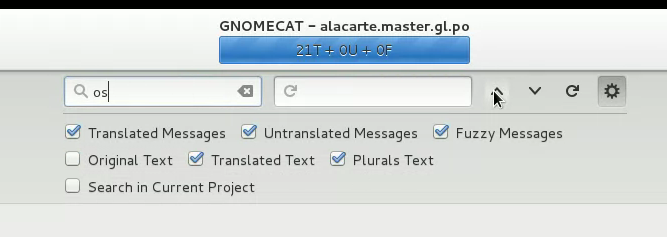
\includegraphics[width=0.8\textwidth]{img/curso2014_it2_search.png}
    \caption{Barra de busca}
    \label{fig:ui:v2:search}
\end{figure}

Para construír esta barra empregamos o widget \lstinline{GTK.SearchBar}. Creamos un modo de busca normal e un modo avanzado. O modo normal amosa unha caixa de texto para introducir a busca e frechas para avanzar na busca, e o modo avanzado engade unha segunda entrada de texto e un botón para a opción de buscar e remplazar e permite seleccionar que cadeas queremos incluír na busca.

Esta interface, aínda que máis pulida cá anterior, presentaba problemas á hora de editar longas cadeas de texto. Ademais, non deixaba demasiado espazo para engadir información sobre as cadeas. Debido a isto escribimos un artigo con algúns mockups baseados en algúns deseños feitos para GTranslator. Durante o GSoC 2014 creamos a que está pensada como a interface definitiva do programa.

\subsubsection{Terceira Versión}
Para a realización desta terceira versión e definitiva intentamos poñernos en contacto cos deseñadores de GNOME para que nos axuden co deseño da nova interface. Ante a baixa participación neste sentido por parte dos deseñadores, usamos uns deseños feitos por Daniel Korostil para un redeseño de GTranslator que nunca chegou a implementarse. Baseándonos nestes mockups e en ideas propias creamos un novo concepto de interface que ten como idea principal a de intentar eliminar onde sexa posible calquera diálogo externo ó programa.

A ventá pasa a compoñerse dunha barra de ferramentas integrada nun \lstinline{GTK.HeaderBar}, unha barra de notificacións e un conxunto de paneis.

\begin{figure}[h!]
  \centering
    
\includegraphics[width=0.8\textwidth]{img/editheaderbar.png}
    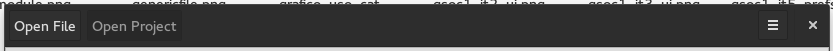
\includegraphics[width=0.8\textwidth]{img/openedfilesheaderbar.png}
    
\includegraphics[width=0.8\textwidth]{img/preferencesheaderbar.png}
    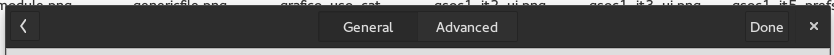
\includegraphics[width=0.8\textwidth]{img/profileheaderbar.png}
    \caption{Diferentes Barras de Ferramentas}
    \label{fig:ui:v3:headerbar}
\end{figure}

A barra de ferramentas é dinámica e os botóns que amosa dependen de que pantalla se estea mostrando no programa. Esta é unha das suxerencias que a Guía de Interfaces Humanas de GNOME fai.

Para lograr isto dentro do \lstinline{GTK.HeaderBar} introducimos un widget denominado \lstinline{GTK.Notebook}. Este widget é o mesmo que se empregaba en versións anterior da interface para ter diferentes ficheiros abertos en outras tantas lapelas, pero empregando a opción que este incorpora de ocultar as lapelas. Desta forma, cada páxina do GTK.Notebook é unha das opcións da barra de ferramentas. Na Figura~\ref{fig:ui:v3:headerbar} podemos ver algúnhas das diferentes formas da barra de ferramentas.

Os botóns da barra de tarefas xeran accións de GTK que serán manexadas pola ventá. A ventá manexará estas accións delegando no panel que esté activo nese momento facendo uso do patrón \emph{State}\cite{book:gang4pat}. No Fragmento de Código~\ref{lst:oneditsave} pódese ver un exemplo da implementación dun dos manexadores.

\lstset{language=[sharp]C}
\begin{lstlisting}[label=lst:oneditsave,caption=Implemenación do manexador da acción gardar]
  private void on_edit_save ()
  {
    (window_panels.get_nth_page (window_panels.page) as Panel).on_edit_save (this);
  }
\end{lstlisting}

Tamén empregamos un GTK.Notebook para cambiar entre paneis. Os paneis son as diferentes pantallas que se poden ver no programa. Desta forma, temos un panel para abrir ficheiros, un panel para as preferencias e un panel para editar os ficheiros entre outros. Na implementación cada panel ten que implementar a interface Panel. Esta interface pide que se defina un tipo de barra de tarefas e dá unha implementación xenérica ós manexadores das accións da ventá. Cada panel será libre de aportar unha implementación especifica destas accións. Na seguinte sección trataranse en detalle cada un dos paneis da interface.

En canto á barra de notificación, é a resposta que damos á necesidade de avisar ó usuario de certos eventos do programa. Por exemplo, avisamos ó usuario que está introducindo unha busca, de que non existe ningunha cadea que cumpra o criterio ou, se este está avanzando polas cadeas, que xa chegou á última. Para implementar esta parte fixemos uso do widget \lstinline{GTK.InfoBar}. Amosamos a notificación durante unha certa cantidade de tempo e despois ocultámolo. Na Figura~\ref{fig:ui:v3:infobar} vemos unha captura da barra de notificación.

\begin{figure}[h!]
  \centering
    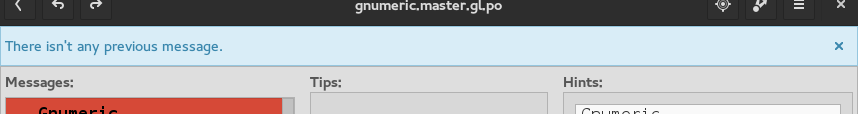
\includegraphics[width=0.7\textwidth]{img/gsoc2_it3_ui.png}
    \caption{Barra de Notificacións}
    \label{fig:ui:v3:infobar}
\end{figure}

Por último, tamén engadimos un menú de aplicación que permite acceder ó panel de preferencias, pechar o programa e iniciar un dialogo para obter información sobre quen fixo GNOMECAT e a súa licenza, entre outros. O uso de menús de aplicación en GNOME é unha recomendación da súa Guía de Interfaces Humanas. Pódese acceder ó menú de aplicación dende GNOME facendo click na icona da aplicación na barra superior do entorno de ventás.

\subsection{Paneis}
Os paneis empregados no programa son os seguintes:

\subsubsection{Panel de Benvida}

O panel de benvida amósaselle ó usuario cando non hai ningún perfil dispoñible no programa. Isto sucede se é a primeira vez que se inicia o programa ou se de forma externa se borrou a información dos perfiles.

\begin{figure}[h!]
    \centering
    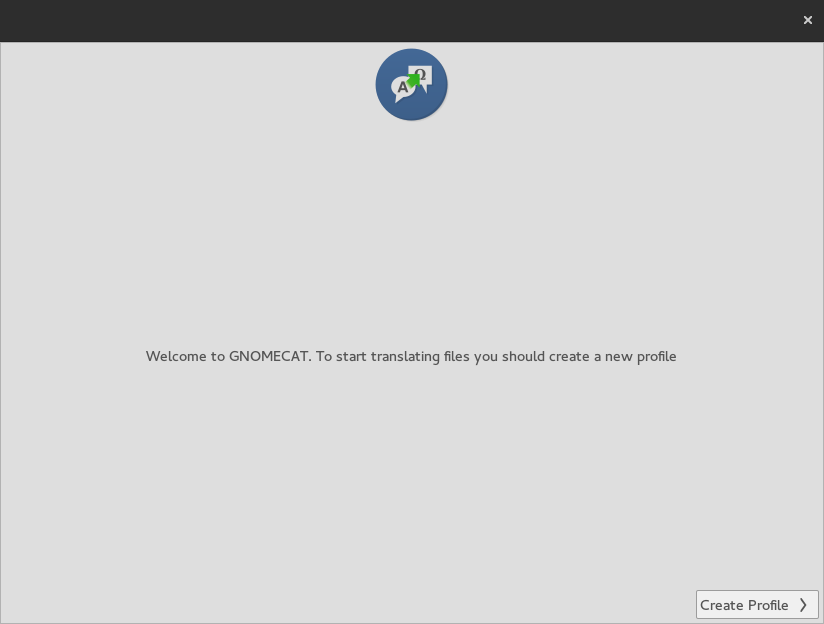
\includegraphics[width=0.8\textwidth]{img/panel_benvida.png}
    \caption{Panel de Benvida}
    \label{fig:ui:panel:welcome}
\end{figure}

Como podemos ver na Figura~\ref{fig:ui:panel:welcome}, amósaselle unha mensaxe de información ó usuario permíndolle acceder ó panel de creación do primeiro perfil.

A barra de ferramentas non inclúe ningún botón xa que a interface só permite avanzar cara ó panel de creación do primeiro perfil ou pechar o programa.

\subsubsection{Panel de ficheiros abertos}

Este panel, como o seu nome indica, amosa unha lista de ficheiros abertos. É o que primeiro se amosa cando abrimos o programa e xa temos perfil creado. Ademais, permite abrir novos ficheiros.

\begin{figure}[h!]
    \centering
    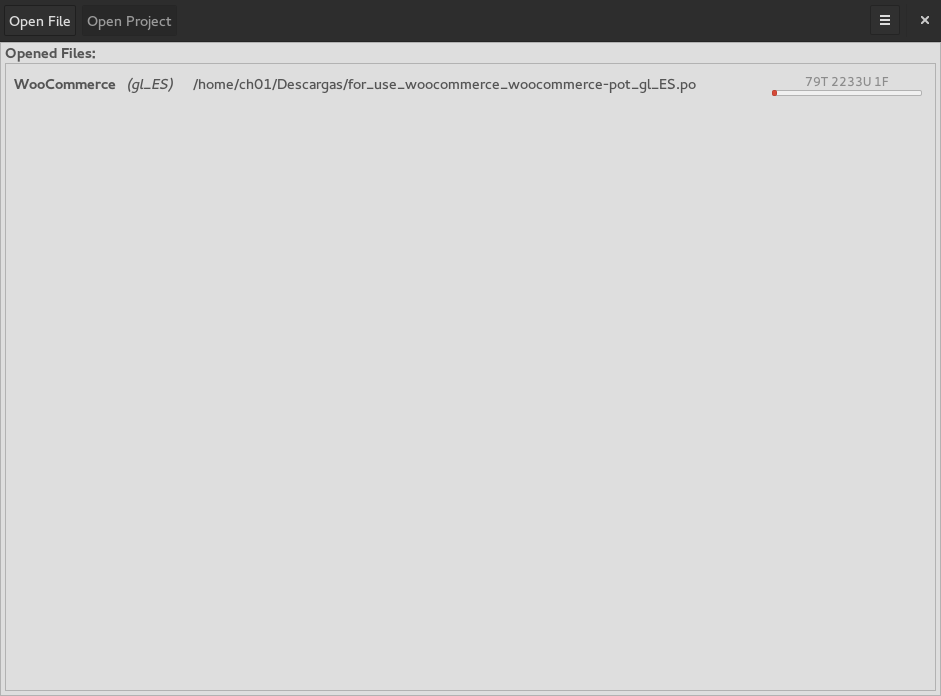
\includegraphics[width=0.8\textwidth]{img/panel_ficheiros_abertos.png}
    \caption{Panel de Ficheiros Abertos}
    \label{fig:ui:panel:openedfiles}
\end{figure}

Na Figura~\ref{fig:ui:panel:openedfiles} pódese ver este panel. Para cada un dos ficheiros abertos amosamos o nome do proxecto segundo aparece nos metadatos do ficheiro PO; a linguaxe deste ficheiro, o path absoluto onde este se atopa e as estatísticas de tradución.

Ademais de permitir abrir un novo ficheiro, a barra de ferramentas tamén permite acceder ó panel de preferencias.

\subsubsection{Panel de abrir ficheiro}

O panel de abrir ficheiros amosa os ficheiros abertos de forma recente e permite abrir novos ficheiros.

Para poder implementar a lista de ficheiros recentes tivemos que crear un widget personalizado. O novo widget emprega a clase \lstinline{GTK.RecentManager}. Esta clase, que funciona empregando o patrón \emph{Singleton}\cite{book:gang4pat}, controla os ficheiros que se abren en todo os sistema. O widget creado conectase á instancia de RecentManager para modificar a lista de ficheiros recentes cada vez que un ficheiro compatible é aberto.

A hora de amosar a información sobre os ficheiros amosamos os mesmos campos que no caso do panel de ficheiros abertos. Isto é debido a que nos dous casos empregamos un GTK.ListBox ao que lle introducimos un widget PoFileRow por cada un dos ficheiros.

\begin{figure}[h!]
  \centering
    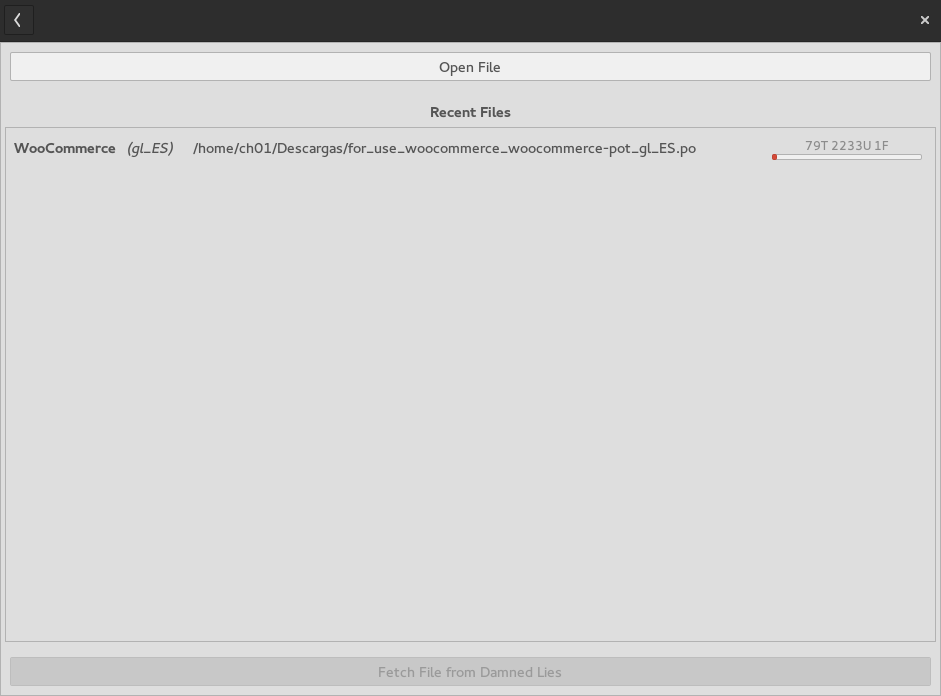
\includegraphics[width=0.8\textwidth]{img/panel_abrir_ficheiro.png}
    \caption{Panel de Abrir Ficheiro}
    \label{fig:ui:panel:openfile}
\end{figure}

Como podemos ver na Figura~\ref{fig:ui:panel:openfile} a barra de ferramentas permite volver a último panel que neste caso sempre será o panel de ficheiros abertos.

\subsubsection{Panel de edición}

O panel de edición é o máis importante deste programa e ao que lle dedicamos máis tempo. Como os seu nome indica permite editar os ficheiros. Está composto de tres columnas, unha lista de mensaxes, unha lista de pistas e unha columna central que contén os consellos, entradas para editar as cadeas e o contexto. As columnas que teñen a lista de mensaxes e de pistas teñen un ancho fixo e a columna central aproveitará todo o espazo restante.

\begin{figure}[hp!]
    \centering
    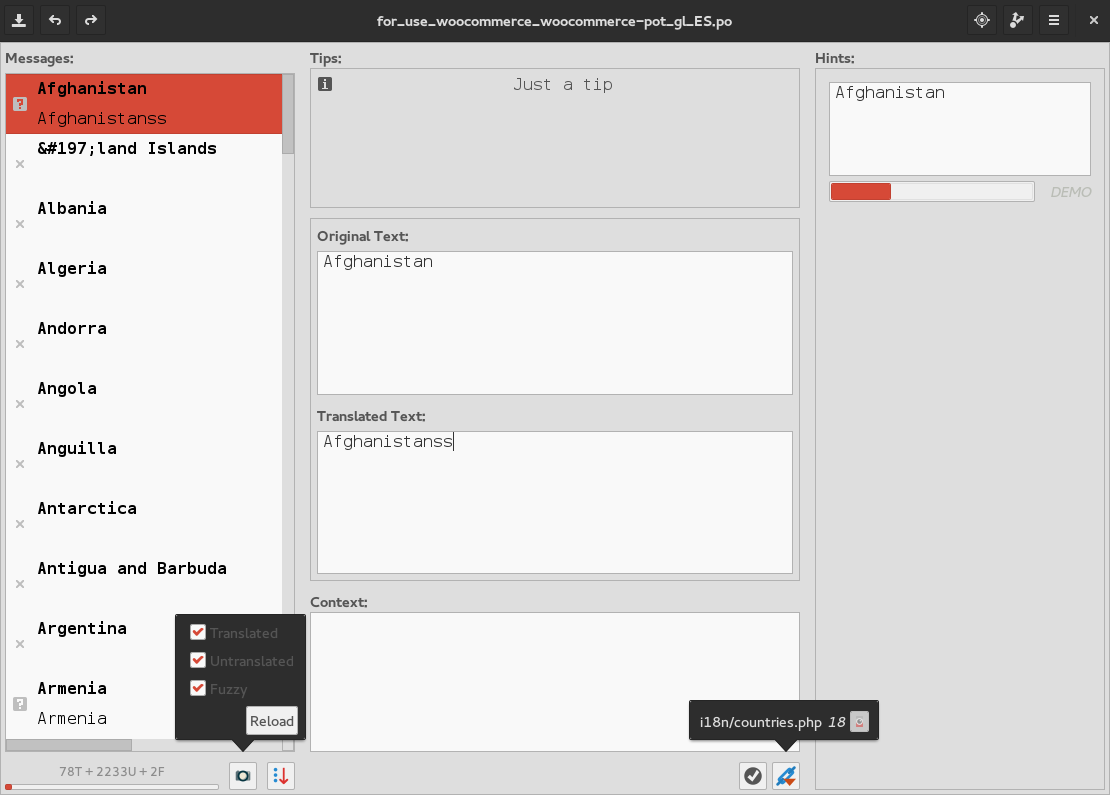
\includegraphics[angle=90,width=\textwidth]{img/panel_edicion.png}
    \caption{Panel de Edición de Ficheiros}
    \label{fig:ui:panel:edit}
\end{figure}

Como se pode comprobar nesta versión da interface, as caixas de edición de cadeas son considerablemente máis grandes que nas outras versións. Na Figura~\ref{fig:ui:panel:edit} podemos ver unha captura deste panel.

A parte que máis traballo nos supuxo foi implementar a lista de mensaxes. Inicialmente deseñamos este \emph{widget} como un \lstinline{GTK.ListBox} coas súas columnas. Este é un widget engadido na versión 3.10 de GTK+ e que empregamos moito no noso programa. A vantaxe de empregalo consiste en que é moi sinxelo personalizar cada columna e aínda que non o usamos no noso programa existiría a posibilidade de engadir columnas de diferentes tipos. O problema que atopamos cando construímos o widget de listar mensaxes con un \lstinline{ListBox} é que este funcionaba realmente mal cando o ficheiro tiña moitas cadeas. Primeiro pensamos que a lentitude debíase ao alto consumo de memoria cando cargabamos un destes ficheiros pero máis tarde falando con algún desenvolvedor de GTK+, démonos conta de que este widget non estaba deseñado para soportar tantas columnas e que debíamos empregar unha alternativa.

A alternativa escollida foi a de empregar un \lstinline{GTK.TreeView}. Este widget si que esta deseñado para soportar gran cantidade de columnas pero a personalización de cada columna e moito máis complicada. Para facelo tivemos que implementar un \lstinline{GTK.CellRenderer} para o renderizado das columnas. Nesta clase especificamos a man onde se debuxa cada elemento da columna e que tamaño ten.

A clase \lstinline{TreeView} incorpora métodos que permiten ordenar e filtrar de forma sinxela as columnas que se amosan neste widget. Isto permitiunos engadir estas opción a nosa interface. Como se pode ver na figura anterior debaixo da lista de mensaxe temos unha barra coas estatísticas do documento e dous botóns un permite filtrar os resultados ocultando ou amosando as cadeas traducidas, sen traducir ou con tradución difusa e o outro permite ordenar as mensaxes amosando primeiro as mensaxes sen traducir, despois as mensaxes con tradución difusa e por último as mensaxes traducidas.

En canto ao widget de lista de pistas, neste caso si que empregamos un \lstinline{GTK.ListBox} xa que o número de columnas nunca vai ser demasiado alto. En cada unha das columnas amosamos a información que temos de cada pista (\lstinline{Hint}). Isto é, a cadea suxerida, a orixe desta pista e a súa precisión. Para amosar a precisión empregamos unha barra de progreso. Ao facer dobre click nos Hints o texto a traducir substituirase polo pista. Ademais incorporamos atallos de teclado para as 4 primeiras pista de forma que se pulsamos as teclas Ctrl e un dos catro primeiros números activarase a correspondente pista.

Dentro da columna central a lista de consellos (\lstinline{Tip}) atopase na parte superior. Esta localización esta pensada para que o tradutor non teña que apartar demasiado a mirada do cadros de edición de mensaxes.

\begin{figure}[h!]
    \centering
    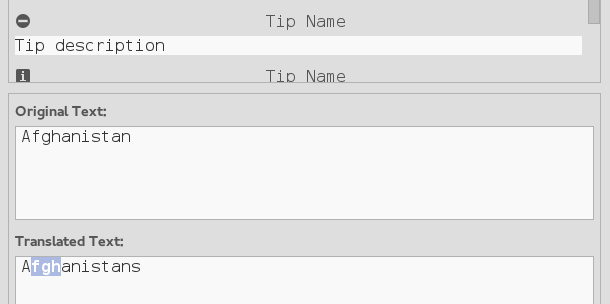
\includegraphics[width=0.6\textwidth]{img/selectedtip.png}
    \caption{Selección dun consello}
    \label{fig:ui:panel:edit:selectedtip}
\end{figure}

Desta forma cada columna amosará o nome do \lstinline{Tip} e o seu nivel de gravidade. O nome do consello debe ser suficiente para que o usuario se de conta do erro ao que se refire o consello. En caso de non ser suficiente o usuario pode premer encima do consello nese caso amosarase a descrición do consello e resaltarase a parte do texto á que refire o mesmo. Na Figura~\ref{fig:ui:panel:edit:selectedtip} podes mover ver unha captura desta situación.

Os cadros que permiten ver a cadeda orixinal están construídos co widget \lstinline{GTK.SourceView} este widget que non é parte da librería GTK extende o widget GTK.TextView e permite facer de forma sinxela, desfacer e refacer accións, resaltado de sintaxe e resaltado de espacios en blanco entre outros. Na Figura~\ref{fig:ui:panel:edit:pluralbox} podemos ver unha cadea con resaltado de sintaxe e de espazos en branco.

\begin{figure}[h!]
    \centering
    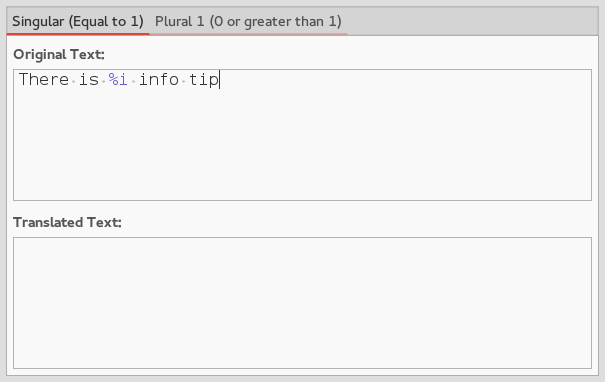
\includegraphics[width=0.6\textwidth]{img/editbox.png}
    \caption{Cadro de edición de mensaxes con plurais}
    \label{fig:ui:panel:edit:pluralbox}
\end{figure}

No caso de que a mensaxes a traducir teña plurais amosaremos cada plural nunha lapela. Como se pode ver na Figura~\ref{fig:ui:panel:edit:pluralbox}, no texto que amosa a lapela, aparte do número de plural amosaremos unha etiqueta explicando a que números se refire ese plural.

Debaixo do cadro de texto que amosa o contexto, temos botóns para ver as orixes da mensaxe actual e para cambiar o estado da mensaxe entre traducida e difusa. Para ver as orixes tamén se usa un widget \lstinline{GTK.Popover}.

A barra de tarefas ten botóns para volver a lista de ficheiros, gardar o ficheiro actual, facer e desfacer as accións, buscar, navegar a través do documento e ver as preferencias. Os botóns de volver a lista de ficheiros e de gardar son intercambiables de forma que so un deles se amosa en cada momento. Se o ficheiro foi modificado o botón que se amosa e o de gardar. Desta forma para ir a lista de ficheiros gardados deberemos salvar os cambios.


\subsubsection{Panel de Preferencias}
O panel de preferencias permite modificar como se algunhas opcións do programa, manexar os perfiles e activar ou desactivar plugins. Como podemos ver nas capturas da Figura~\ref{fig:ui:panel:preferences} temos tres pantallas para modificar as preferencias do programa.

\begin{figure}[h!]
  \centering
  \begin{subfigure}[b]{0.56\textwidth}
    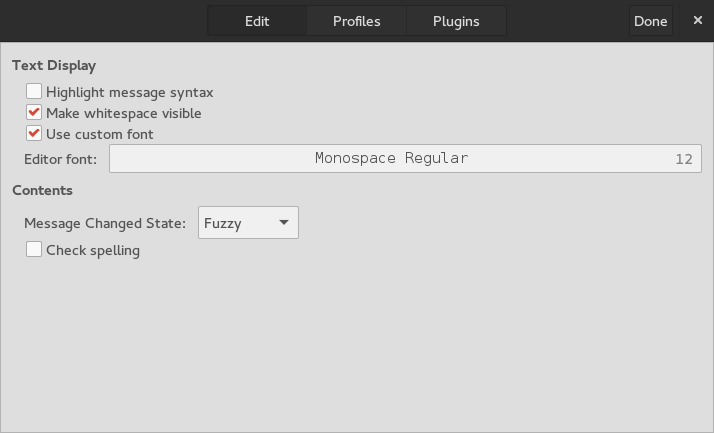
\includegraphics[width=\textwidth]{img/panel_preferencias_edicion.png}
    \caption{Edición}
  \end{subfigure}
  \begin{subfigure}[b]{0.56\textwidth}
    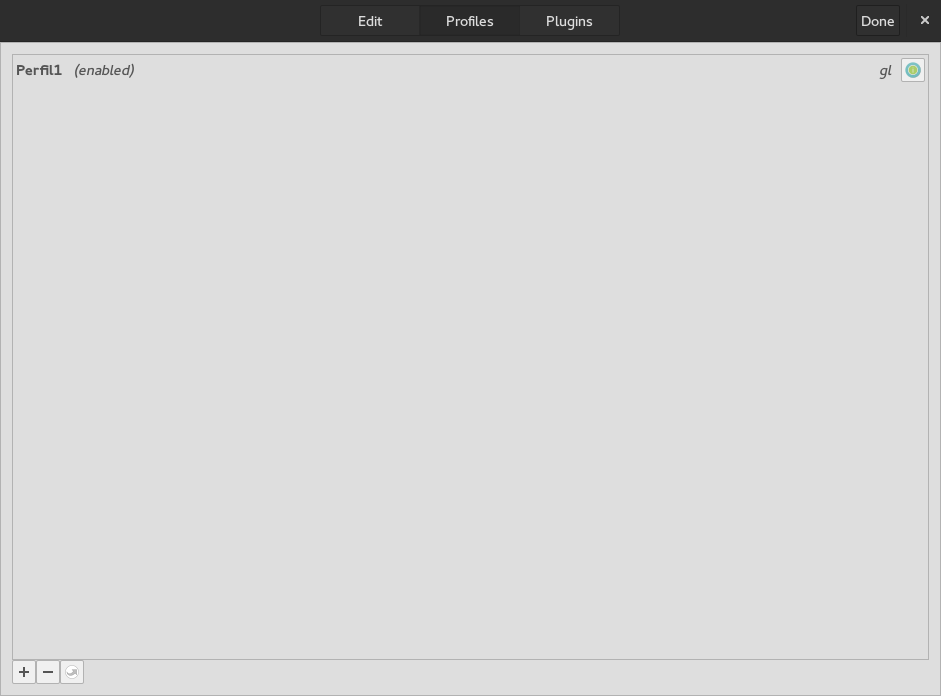
\includegraphics[width=\textwidth]{img/panel_preferencias_perfiles.png}
    \caption{Perfiles}
  \end{subfigure}
  \begin{subfigure}[b]{0.56\textwidth}
    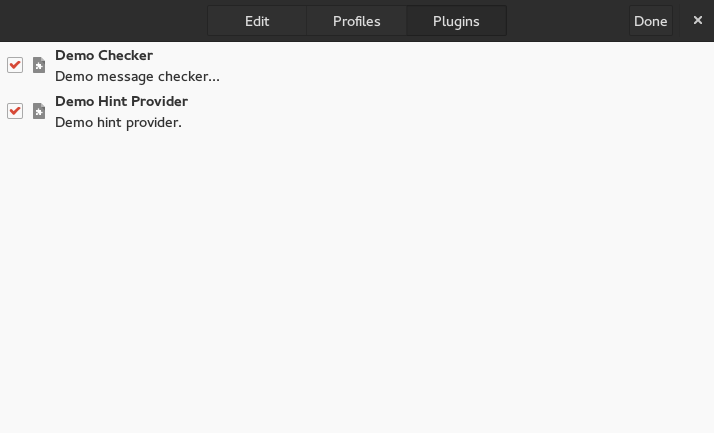
\includegraphics[width=\textwidth]{img/panel_preferencias_plugins.png}
    \caption{Plugins}
  \end{subfigure}
    \caption{Partes do panel preferencias}
    \label{fig:ui:panel:preferences}
\end{figure}

Navegamos entre estas tres pantallas empregando un widget \lstinline{GTK.StackSwitcher} incrustado na barra de ferramentas.

A pantalla de edición permite modificar o tipo de letra de algunhas partes do programa, o uso de resaltado de sintaxe ou o de espazos en branco. Ademais permite establecer cal é o estado ao que pasa unha cadea cando se traduce. O panel de perfil permite ver os perfiles existentes crear novos perfiles a través do panel de perfil, modificalos, eliminalos e activalos. Por último ca pantalla de plugins podemos ver a lista de plugins existentes e activalos ou desactivalos.


\subsubsection{Panel de Perfil}
O panel perfil permite a creación e modificación de perfiles. Esta dividido en dous subpaneis, un cos datos básicos do perfil e outro con datos avanzados. Estes dous paneis pódense ver na Figura~\ref{fig:ui:panel:profile}.
\begin{figure}[h!]
  \centering
  \begin{subfigure}[b]{0.5\textwidth}
    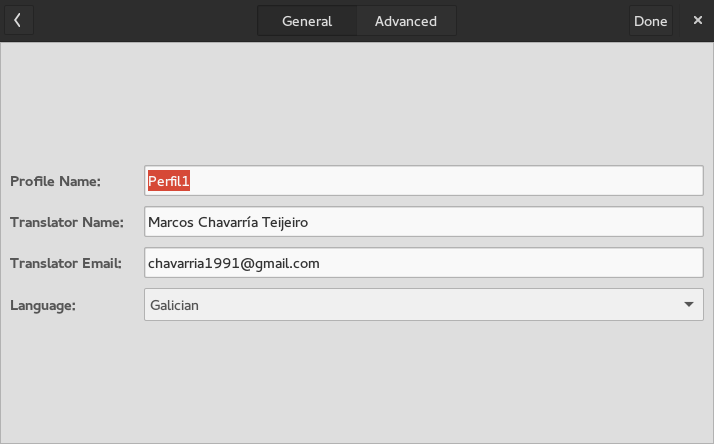
\includegraphics[width=\textwidth]{img/panel_pefil_xeral.png}
    \caption{Opcións básicas}
  \end{subfigure}
  \begin{subfigure}[b]{0.5\textwidth}
    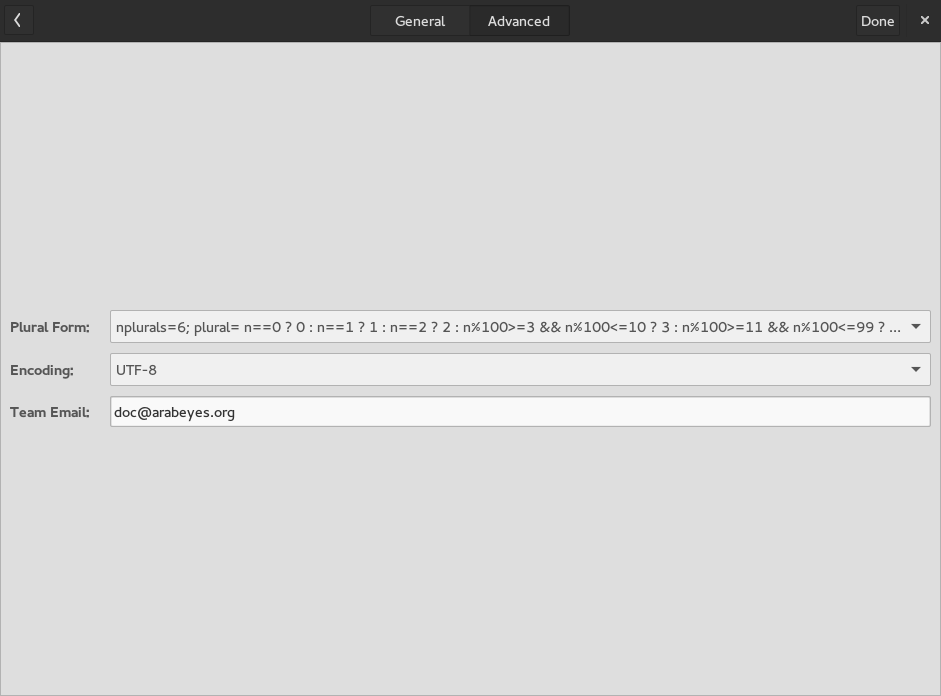
\includegraphics[width=\textwidth]{img/panel_perfil_avanzado.png}
    \caption{Opcións Avanzadas}
  \end{subfigure}
    \caption{Panel de perfil}
    \label{fig:ui:panel:profile}
\end{figure}

Esta división intenta mellorar a experiencia de usuario pois os valores avanzados autocompletanse cos valores por defecto no momento no que se selecciona a linguaxe.

\section{Navegación e Busca a través do documento}

Unha das partes importantes para facilitar a usabilidade da aplicación é que esta permita que o tradutor navegue polo ficheiro e busque termos de forma sinxela e rápida. Para facer isto creamos a clase abstracta \lstinline{Navigator}. Esta clase ten métodos sen argumentos que permiten avanzar ao seguinte, ao anterior, ao primeiro ou ao último elemento. O valor de volta destes métodos é un valor booleano que indica se esta operación foi posible.

\begin{figure}[h!]
  \centering
  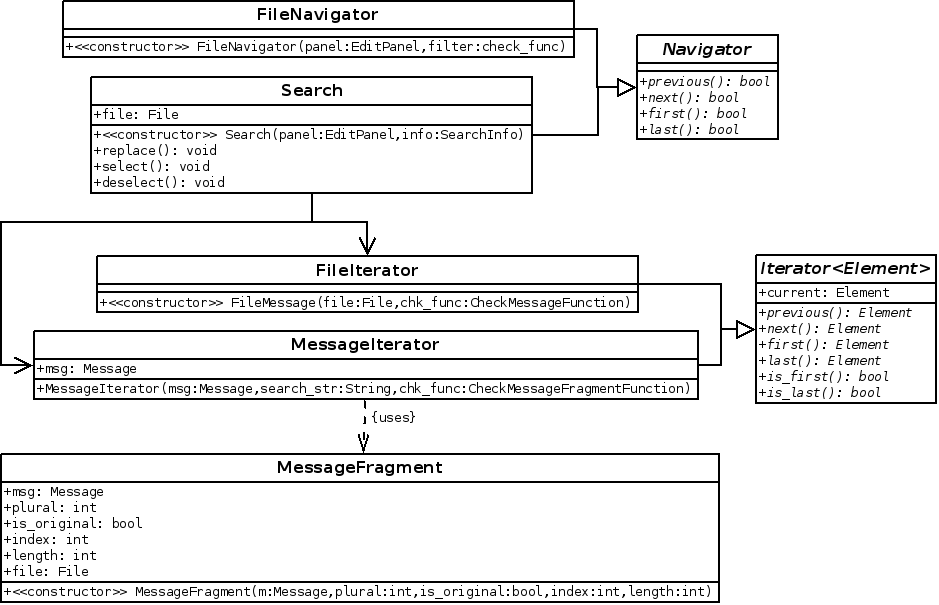
\includegraphics[width=\textwidth]{img/navigator_diagram.png}
  \caption{Diagrama de Clases de Navegación e Busca}
  \label{fig:nav:diagram}
\end{figure}

Para a implementación a busca dentro do documento creamos a clase \lstinline{Search}. Para implementar os métodos para avanzar a través dos resultados da busca empregamos dous iteradores, un que itera dentro dos mensaxes que cumpren os criterios e outro que itera dentro dos fragmentos das mensaxes.

Como podemos ver na Figura~\ref{fig:nav:diagram} os iteradores teñen métodos para conseguir o elemento actual, o primeiro, o último, o seguinte e o anterior. Ademais incorporan metodos para comprobar se o elemento actual é o último ou o primeiro.

As buscas permiten especificar o estado das mensaxes que queremos buscar e se o texto de busca está na cadea orixinal ou na traducida e se está na forma singular ou na plural. esta forma cando se inicia unha busqueda crease un iterador de ficheiro que itera entre os mensaxes que cumpren os requisitos e por cada mensaxe que cumpra os requisitos creamos un iterador de mensaxe que iterará devolvendo os fragmentos de mensaxe que cumpran os requisitos. Un \lstinline{MessageFragment} inclúe unha mensaxe, a forma plural do fragmento, se o fragmento está na cadea orixinal ou na tradución e o índice e lonxitude do fragmento.

Para seleccionar un fragmento da busca empregamos o método \lstinline{select()} do panel de edición.

En canto a implementación da navegación entre ficheiros a clase FileNavigator empregouse os métodos propios do widget TreeView de GTK. Créanse catro navegadores deste tipo un para as cadeas traducidas, outro para as cadeas sen traducir, outro para as cadeas con tradución difusa e outro para calquera cadea.

\section{Preferencias}
Necesitamos almacenar certas opcións do programa como pode ser o tipo e tamaño da letra a empregar ou se facemos resaltado e sintaxe. Para gardar toda esta información e que este dispoñible entre diferentes sesións do programa empregamos GSettings. GSettings é unha API para a xestión de configuración que forma parte do modulo GIO (GNOME Input/Output) dentro de GLib.

GSettings prové de métodos para obter e almacenar valores a partir dunha clave. Para almacenar estes valores soporta varios sistemas. Nós en concreto usamos o estándar en GNOME, \emph{dconf}. Este sistema está altamente optimizado para facer lecturas (o caso de uso máis habitual) de valores de configuración. Para usar GSettings debemos crear un ficheiro coas claves e tipos dos valores que imos empregar. No Fragmento de Código~\ref{lst:gsettings} podemos ver unha parte deste ficheiro.

\begin{lstlisting}[language=XML,label=lst:gsettings,caption=Fragmento da dos esquemas creados de GSettings]
<?xml version="1.0" encoding="UTF-8"?>
<schemalist>
  <schema path="/org/gnome/gnomecat/editor/" id="org.gnome.gnomecat.Editor">
    <key name="custom-font" type="b">
      <default>true</default>
      <summary>Use custom font.</summary>
      <description></description>
    </key>
    <key name="message-changed-state" type="s">
      <choices>
        <choice value='fuzzy'/>
        <choice value='translated'/>
      </choices>
      <default>'fuzzy'</default>
      <summary>Message Changed State</summary>
      <description>The state to set when a message is translated.</description>
    </key>
    [...]
  </schema>
  [...]
</schemalist>
\end{lstlisting}

Este ficheiro temos que compilalo e instalalo cas ferramentas que nos dá o módulo. Unha vez instalado obtemos unha instancia da clase GSettings que emprega o patrón Singleton e usamos esta instancia para obter e almacenar os valores.

Unha das vantaxes de GSettings é que permite enlazar unha propiedade dun obxecto de GObject con un valor de GSettings de forma que se modificamos o valor dun dos dous o outro vese reflexado. Empregamos esta característica para implementar a interface de preferencias na nosa aplicación de forma sinxela.

\subsection{Módulo de Perfiles}
Como vimos anteriormente ao falar da interface gráfica, os perfiles permiten configurar o nome e email co que se gardan os ficheiros e a linguaxe actual. Aínda que poden existir varios perfiles gardados so un estará activo en cada momento. Para almacenar estes perfiles tamén empregaremos GSettings.

\section{Plugins}
Os plugins permiten estender o programa engadíndolle funcionalidade. Dous dos puntos máis sinxelos para engadir funcionalidade son as pistas e os consellos. Estes dous elementos que están pensados para axudar os tradutores son aportados polos plugins. Existen dúas sinais de nomes \lstinline{check_message} e \lstinline{provide_hints} que son usadas para crear instancias de pistas e de consellos. Estas sinais son chamadas dende os plugins.

Para implementar estes plugins empregamos a biblioteca \emph{LibPeas}. Esta biblioteca foi creada para poder incluír extensións en GEdit, o editor de texto de GNOME. Trátase dun motor de plugins baseado en GObject. Permite a carga de plugins en varios linguaxes de programación como Vala, C, Python ou JavaScript.

Os plugins son unha unidade de compilación diferente ao programa principal. Para que desde esta unidade independente de compilación coñeza parte da API creada para ficheiros, perfiles e linguaxes debemos incluír estes ficheiros tamén nesta unidade de compilación. Creamos ademais unha pequena interface que inclúe as dúas sinais que citamos anteriormente. Esta interface é implementada pola clase aplicación.

A biblioteca LibPeas emprega o patrón Singleton para darnos unha instancia dun motor de plugins. A este motor temos que indicarlle a ruta do sistema onde ten que buscar os plugins e cargar os plugins que atopen. Ademais cargamos un obxecto de clase

Para implementar un plugin temos que crear dous ficheiros. O primeiro ficheiro contén no nome do plugin información sobre o plugin como a descrición, o autor ou autores e o Copyright. No Fragmento de Código~\ref{lst:plugin:metadata} pódese ver un exemplo deste ficheiro.

\begin{lstlisting}[label=lst:plugin:metadata,caption=Ficheiro de metadatos do plugin]
[Plugin]
Module=demochecker
Name=Demo Checker
Description=Demo message checker...
Authors=Marcos Chavarría Teijeiro <chavarria1991@gmail.com>
Copyright=Copyright (C) 2014 Marcos Chavarría Teijeiro
\end{lstlisting}

O outro ficheiro é a implementación do propio plugin. Debemos implementar unha ou máis extensións e unha función onde as rexistraremos. A función ten que ter o nome \lstinline{peas_register_types()} e usará a etiqueta \lstinline{ModuleInit} de forma que se executará cando se inicialice o módulo.

\begin{lstlisting}[label=lst:plugin:code,caption=Fragmento da implementación do plugin DemoChecker]
public class DemoChecker : Peas.ExtensionBase,  Peas.Activatable
{
    public Object object  { owned get; construct; }

    public void activate ()
    {
      (object as GNOMECAT.API).check_message.connect (on_check_message);
    }

    public void deactivate ()
    {
      (object as GNOMECAT.API).check_message.disconnect (on_check_message);
    }

    public void update_state ()
    {
    }

    [...]
}

[ModuleInit]
public void peas_register_types (GLib.TypeModule module)
{
  var objmodule = module as Peas.ObjectModule;
  objmodule.register_extension_type (typeof (Peas.Activatable),
                                     typeof (DemoPlugins.DemoChecker));
}
\end{lstlisting}

Para implementar unha extensión temos que implementar unha clase que implemente a interface Activable e herede da clase ExtensionBase. A interface Activable inclúe os métodos que se executarán cando se active e desactive o plugin. No Fragmento de Código~\ref{lst:plugin:code} amosase parte do código empregado para o plugin de exemplo \emph{DemoPlugin}. Podemos ver como nos métodos para activar e desactivar conectamos e desconectamos a sinal \lstinline{check_message} para poder xerar os Tips de exemplo.


        \chapter{Conclusións e Traballo futuro}

\section{Conclusións}

\section{Traballo Futuro}
Como calquera proxecto de software libre este programa é un proxecto inconcluso. Por unha parte moitos dos requisitos establecidos ao inicio do proxecto ou presentan deficiencias ou están elaborados con pouco detalle. Ademais aínda que neste proxecto a interface gráfica supuxo un esforzo importante, aínda hai algunhas partes que poden ser mellorables.

Por outro lado as contribución externas a este proxecto foron moi limitadas pois so contribuiron dúas persoas con cambios triviales. Para que un proxecto destas caracteristicas teña futuro é necesario crear unha comunidade arredor del. Polo que unha das liñas de traballo ten que ser buscar contribuidores para o proxecto e integralo dentro da infraestructura de GNOME.

Se falamos de liñas de traballo en canto a implementación de novas caracteristicas existen varias lineas de traballo moi interesantes:

\paragraph{Integración con Damned Lies.} Damned Lies é a plataforma oficial de GNOME para xestionar as traducións. Nela podense baixar os ficheiros para traducir, subir os ficheiros traducidos, revisar os mesmos, e ver as estatisticas xerais de tradución para cada linguaxe. Sería realmente útil que todas estas tarefas se puidesen facer dende GNOMECAT. Para isto non so bastaría con implementar novas vistas en GNOMECAT senón tamén a creación dunha API pública para a plataforma web Damned Lies que está escrita en Python empregando o framework Django.

\paragraph{Glosario.} Implementación dun glosario de termos na interface de edición de GNOMECAT. Este glosario debería permitir importar e exportar diversas bases de datos tanto online como offline.

\paragraph{Previsualización das traducións.} Como xa se comentou anteriormente esta é unha caracteristica moi interesante para unha ferramenta CAT pois permite que os traductores vexan como pode quedar a tradución no programa final. Aínda que existen varias alternativas para implementar esta funcionalidade semella que a máis axeitada para tecnoloxías GNOME é empregar o motor de renderizado Glade como se fixo na aplicación web Deckard.


  % INCLUIMOS LOS APÉNDICES...
        \appendix
        \chapter{Escoller a licencia do programa}

A hora de escoller unha licencia para o novo programa temos que ter en conta as licencias das bibliotecas empregadas no noso programa. Na siguente lista podense ver as bibliotecas empregadas para o programa así como a licencia de cada unha delas.

\begin{itemize}
  \item \textbf{GLib} GNU Lesser General Public License v2.1
  \item \textbf{GTK+} GNU Lesser General Public License v2.1
  \item \textbf{LibGee}  GNU Lesser General Public License v2.1
  \item \textbf{LibPeas} GNU Lesser General Public License v2.1
  \item \textbf{GettextPo} GNU General Public License v2
  \item \textbf{GTKSourceView} GNU Lesser General Public License v2.1
  \item \textbf{JSON-GLib} GNU Lesser General Public License v2.1
\end{itemize}

Como podemos ver excepto a biblioteca GettextPO, que emprega unha licencia GNU GPLv2, o resto de bibliotecas empregadas usan unha licencia GNU LGPL v2.1. A licencia GNU Lesser GPL permite empregar calquera licencia en productos derivados. Por outra parte a licencia GNU GPL v.2 obliga a empregar a licencia GNU GPL v2 ou versións posteriores da mesma licencia.

No noso caso eleximos a licencia GNU General Public Licence v3 que é unha versión máis actualizada da licencia para programas de GNU. No seguinte apéndice podese ver o texto completo desta licecia.


       % \section{Licencia GPLv3}
\begin{center}
{\parindent 0in

Copyright \copyright\  2007 Free Software Foundation, Inc. \texttt{http://fsf.org/}

\bigskip
Everyone is permitted to copy and distribute verbatim copies of this

license document, but changing it is not allowed.}

\end{center}

\begin{center}
{\Large \sc Preamble}
\end{center}
The GNU General Public License is a free, copyleft license for
software and other kinds of works.

The licenses for most software and other practical works are designed
to take away your freedom to share and change the works.  By contrast,
the GNU General Public License is intended to guarantee your freedom to
share and change all versions of a program--to make sure it remains free
software for all its users.  We, the Free Software Foundation, use the
GNU General Public License for most of our software; it applies also to
any other work released this way by its authors.  You can apply it to
your programs, too.

When we speak of free software, we are referring to freedom, not
price.  Our General Public Licenses are designed to make sure that you
have the freedom to distribute copies of free software (and charge for
them if you wish), that you receive source code or can get it if you
want it, that you can change the software or use pieces of it in new
free programs, and that you know you can do these things.

To protect your rights, we need to prevent others from denying you
these rights or asking you to surrender the rights.  Therefore, you have
certain responsibilities if you distribute copies of the software, or if
you modify it: responsibilities to respect the freedom of others.

For example, if you distribute copies of such a program, whether
gratis or for a fee, you must pass on to the recipients the same
freedoms that you received.  You must make sure that they, too, receive
or can get the source code.  And you must show them these terms so they
know their rights.

Developers that use the GNU GPL protect your rights with two steps:
(1) assert copyright on the software, and (2) offer you this License
giving you legal permission to copy, distribute and/or modify it.

For the developers' and authors' protection, the GPL clearly explains
that there is no warranty for this free software.  For both users' and
authors' sake, the GPL requires that modified versions be marked as
changed, so that their problems will not be attributed erroneously to
authors of previous versions.

Some devices are designed to deny users access to install or run
modified versions of the software inside them, although the manufacturer
can do so.  This is fundamentally incompatible with the aim of
protecting users' freedom to change the software.  The systematic
pattern of such abuse occurs in the area of products for individuals to
use, which is precisely where it is most unacceptable.  Therefore, we
have designed this version of the GPL to prohibit the practice for those
products.  If such problems arise substantially in other domains, we
stand ready to extend this provision to those domains in future versions
of the GPL, as needed to protect the freedom of users.

Finally, every program is threatened constantly by software patents.
States should not allow patents to restrict development and use of
software on general-purpose computers, but in those that do, we wish to
avoid the special danger that patents applied to a free program could
make it effectively proprietary.  To prevent this, the GPL assures that
patents cannot be used to render the program non-free.

The precise terms and conditions for copying, distribution and
modification follow.

\begin{center}
{\Large \sc Terms and Conditions}
\end{center}


\begin{enumerate}

\addtocounter{enumi}{-1}

\item Definitions.

``This License'' refers to version 3 of the GNU General Public License.

``Copyright'' also means copyright-like laws that apply to other kinds of
works, such as semiconductor masks.

``The Program'' refers to any copyrightable work licensed under this
License.  Each licensee is addressed as ``you''.  ``Licensees'' and
``recipients'' may be individuals or organizations.

To ``modify'' a work means to copy from or adapt all or part of the work
in a fashion requiring copyright permission, other than the making of an
exact copy.  The resulting work is called a ``modified version'' of the
earlier work or a work ``based on'' the earlier work.

A ``covered work'' means either the unmodified Program or a work based
on the Program.

To ``propagate'' a work means to do anything with it that, without
permission, would make you directly or secondarily liable for
infringement under applicable copyright law, except executing it on a
computer or modifying a private copy.  Propagation includes copying,
distribution (with or without modification), making available to the
public, and in some countries other activities as well.

To ``convey'' a work means any kind of propagation that enables other
parties to make or receive copies.  Mere interaction with a user through
a computer network, with no transfer of a copy, is not conveying.

An interactive user interface displays ``Appropriate Legal Notices''
to the extent that it includes a convenient and prominently visible
feature that (1) displays an appropriate copyright notice, and (2)
tells the user that there is no warranty for the work (except to the
extent that warranties are provided), that licensees may convey the
work under this License, and how to view a copy of this License.  If
the interface presents a list of user commands or options, such as a
menu, a prominent item in the list meets this criterion.

\item Source Code.

The ``source code'' for a work means the preferred form of the work
for making modifications to it.  ``Object code'' means any non-source
form of a work.

A ``Standard Interface'' means an interface that either is an official
standard defined by a recognized standards body, or, in the case of
interfaces specified for a particular programming language, one that
is widely used among developers working in that language.

The ``System Libraries'' of an executable work include anything, other
than the work as a whole, that (a) is included in the normal form of
packaging a Major Component, but which is not part of that Major
Component, and (b) serves only to enable use of the work with that
Major Component, or to implement a Standard Interface for which an
implementation is available to the public in source code form.  A
``Major Component'', in this context, means a major essential component
(kernel, window system, and so on) of the specific operating system
(if any) on which the executable work runs, or a compiler used to
produce the work, or an object code interpreter used to run it.

The ``Corresponding Source'' for a work in object code form means all
the source code needed to generate, install, and (for an executable
work) run the object code and to modify the work, including scripts to
control those activities.  However, it does not include the work's
System Libraries, or general-purpose tools or generally available free
programs which are used unmodified in performing those activities but
which are not part of the work.  For example, Corresponding Source
includes interface definition files associated with source files for
the work, and the source code for shared libraries and dynamically
linked subprograms that the work is specifically designed to require,
such as by intimate data communication or control flow between those
subprograms and other parts of the work.

The Corresponding Source need not include anything that users
can regenerate automatically from other parts of the Corresponding
Source.

The Corresponding Source for a work in source code form is that
same work.

\item Basic Permissions.

All rights granted under this License are granted for the term of
copyright on the Program, and are irrevocable provided the stated
conditions are met.  This License explicitly affirms your unlimited
permission to run the unmodified Program.  The output from running a
covered work is covered by this License only if the output, given its
content, constitutes a covered work.  This License acknowledges your
rights of fair use or other equivalent, as provided by copyright law.

You may make, run and propagate covered works that you do not
convey, without conditions so long as your license otherwise remains
in force.  You may convey covered works to others for the sole purpose
of having them make modifications exclusively for you, or provide you
with facilities for running those works, provided that you comply with
the terms of this License in conveying all material for which you do
not control copyright.  Those thus making or running the covered works
for you must do so exclusively on your behalf, under your direction
and control, on terms that prohibit them from making any copies of
your copyrighted material outside their relationship with you.

Conveying under any other circumstances is permitted solely under
the conditions stated below.  Sublicensing is not allowed; section 10
makes it unnecessary.

\item Protecting Users' Legal Rights From Anti-Circumvention Law.

No covered work shall be deemed part of an effective technological
measure under any applicable law fulfilling obligations under article
11 of the WIPO copyright treaty adopted on 20 December 1996, or
similar laws prohibiting or restricting circumvention of such
measures.

When you convey a covered work, you waive any legal power to forbid
circumvention of technological measures to the extent such circumvention
is effected by exercising rights under this License with respect to
the covered work, and you disclaim any intention to limit operation or
modification of the work as a means of enforcing, against the work's
users, your or third parties' legal rights to forbid circumvention of
technological measures.

\item Conveying Verbatim Copies.

You may convey verbatim copies of the Program's source code as you
receive it, in any medium, provided that you conspicuously and
appropriately publish on each copy an appropriate copyright notice;
keep intact all notices stating that this License and any
non-permissive terms added in accord with section 7 apply to the code;
keep intact all notices of the absence of any warranty; and give all
recipients a copy of this License along with the Program.

You may charge any price or no price for each copy that you convey,
and you may offer support or warranty protection for a fee.

\item Conveying Modified Source Versions.

You may convey a work based on the Program, or the modifications to
produce it from the Program, in the form of source code under the
terms of section 4, provided that you also meet all of these conditions:
  \begin{enumerate}
  \item The work must carry prominent notices stating that you modified
  it, and giving a relevant date.

  \item The work must carry prominent notices stating that it is
  released under this License and any conditions added under section
  7.  This requirement modifies the requirement in section 4 to
  ``keep intact all notices''.

  \item You must license the entire work, as a whole, under this
  License to anyone who comes into possession of a copy.  This
  License will therefore apply, along with any applicable section 7
  additional terms, to the whole of the work, and all its parts,
  regardless of how they are packaged.  This License gives no
  permission to license the work in any other way, but it does not
  invalidate such permission if you have separately received it.

  \item If the work has interactive user interfaces, each must display
  Appropriate Legal Notices; however, if the Program has interactive
  interfaces that do not display Appropriate Legal Notices, your
  work need not make them do so.
\end{enumerate}
A compilation of a covered work with other separate and independent
works, which are not by their nature extensions of the covered work,
and which are not combined with it such as to form a larger program,
in or on a volume of a storage or distribution medium, is called an
``aggregate'' if the compilation and its resulting copyright are not
used to limit the access or legal rights of the compilation's users
beyond what the individual works permit.  Inclusion of a covered work
in an aggregate does not cause this License to apply to the other
parts of the aggregate.

\item Conveying Non-Source Forms.

You may convey a covered work in object code form under the terms
of sections 4 and 5, provided that you also convey the
machine-readable Corresponding Source under the terms of this License,
in one of these ways:
  \begin{enumerate}
  \item Convey the object code in, or embodied in, a physical product
  (including a physical distribution medium), accompanied by the
  Corresponding Source fixed on a durable physical medium
  customarily used for software interchange.

  \item Convey the object code in, or embodied in, a physical product
  (including a physical distribution medium), accompanied by a
  written offer, valid for at least three years and valid for as
  long as you offer spare parts or customer support for that product
  model, to give anyone who possesses the object code either (1) a
  copy of the Corresponding Source for all the software in the
  product that is covered by this License, on a durable physical
  medium customarily used for software interchange, for a price no
  more than your reasonable cost of physically performing this
  conveying of source, or (2) access to copy the
  Corresponding Source from a network server at no charge.

  \item Convey individual copies of the object code with a copy of the
  written offer to provide the Corresponding Source.  This
  alternative is allowed only occasionally and noncommercially, and
  only if you received the object code with such an offer, in accord
  with subsection 6b.

  \item Convey the object code by offering access from a designated
  place (gratis or for a charge), and offer equivalent access to the
  Corresponding Source in the same way through the same place at no
  further charge.  You need not require recipients to copy the
  Corresponding Source along with the object code.  If the place to
  copy the object code is a network server, the Corresponding Source
  may be on a different server (operated by you or a third party)
  that supports equivalent copying facilities, provided you maintain
  clear directions next to the object code saying where to find the
  Corresponding Source.  Regardless of what server hosts the
  Corresponding Source, you remain obligated to ensure that it is
  available for as long as needed to satisfy these requirements.

  \item Convey the object code using peer-to-peer transmission, provided
  you inform other peers where the object code and Corresponding
  Source of the work are being offered to the general public at no
  charge under subsection 6d.
  \end{enumerate}

A separable portion of the object code, whose source code is excluded
from the Corresponding Source as a System Library, need not be
included in conveying the object code work.

A ``User Product'' is either (1) a ``consumer product'', which means any
tangible personal property which is normally used for personal, family,
or household purposes, or (2) anything designed or sold for incorporation
into a dwelling.  In determining whether a product is a consumer product,
doubtful cases shall be resolved in favor of coverage.  For a particular
product received by a particular user, ``normally used'' refers to a
typical or common use of that class of product, regardless of the status
of the particular user or of the way in which the particular user
actually uses, or expects or is expected to use, the product.  A product
is a consumer product regardless of whether the product has substantial
commercial, industrial or non-consumer uses, unless such uses represent
the only significant mode of use of the product.

``Installation Information'' for a User Product means any methods,
procedures, authorization keys, or other information required to install
and execute modified versions of a covered work in that User Product from
a modified version of its Corresponding Source.  The information must
suffice to ensure that the continued functioning of the modified object
code is in no case prevented or interfered with solely because
modification has been made.

If you convey an object code work under this section in, or with, or
specifically for use in, a User Product, and the conveying occurs as
part of a transaction in which the right of possession and use of the
User Product is transferred to the recipient in perpetuity or for a
fixed term (regardless of how the transaction is characterized), the
Corresponding Source conveyed under this section must be accompanied
by the Installation Information.  But this requirement does not apply
if neither you nor any third party retains the ability to install
modified object code on the User Product (for example, the work has
been installed in ROM).

The requirement to provide Installation Information does not include a
requirement to continue to provide support service, warranty, or updates
for a work that has been modified or installed by the recipient, or for
the User Product in which it has been modified or installed.  Access to a
network may be denied when the modification itself materially and
adversely affects the operation of the network or violates the rules and
protocols for communication across the network.

Corresponding Source conveyed, and Installation Information provided,
in accord with this section must be in a format that is publicly
documented (and with an implementation available to the public in
source code form), and must require no special password or key for
unpacking, reading or copying.

\item Additional Terms.

``Additional permissions'' are terms that supplement the terms of this
License by making exceptions from one or more of its conditions.
Additional permissions that are applicable to the entire Program shall
be treated as though they were included in this License, to the extent
that they are valid under applicable law.  If additional permissions
apply only to part of the Program, that part may be used separately
under those permissions, but the entire Program remains governed by
this License without regard to the additional permissions.

When you convey a copy of a covered work, you may at your option
remove any additional permissions from that copy, or from any part of
it.  (Additional permissions may be written to require their own
removal in certain cases when you modify the work.)  You may place
additional permissions on material, added by you to a covered work,
for which you have or can give appropriate copyright permission.

Notwithstanding any other provision of this License, for material you
add to a covered work, you may (if authorized by the copyright holders of
that material) supplement the terms of this License with terms:
  \begin{enumerate}
  \item Disclaiming warranty or limiting liability differently from the
  terms of sections 15 and 16 of this License; or

  \item Requiring preservation of specified reasonable legal notices or
  author attributions in that material or in the Appropriate Legal
  Notices displayed by works containing it; or

  \item Prohibiting misrepresentation of the origin of that material, or
  requiring that modified versions of such material be marked in
  reasonable ways as different from the original version; or

  \item Limiting the use for publicity purposes of names of licensors or
  authors of the material; or

  \item Declining to grant rights under trademark law for use of some
  trade names, trademarks, or service marks; or

  \item Requiring indemnification of licensors and authors of that
  material by anyone who conveys the material (or modified versions of
  it) with contractual assumptions of liability to the recipient, for
  any liability that these contractual assumptions directly impose on
  those licensors and authors.
  \end{enumerate}

All other non-permissive additional terms are considered ``further
restrictions'' within the meaning of section 10.  If the Program as you
received it, or any part of it, contains a notice stating that it is
governed by this License along with a term that is a further
restriction, you may remove that term.  If a license document contains
a further restriction but permits relicensing or conveying under this
License, you may add to a covered work material governed by the terms
of that license document, provided that the further restriction does
not survive such relicensing or conveying.

If you add terms to a covered work in accord with this section, you
must place, in the relevant source files, a statement of the
additional terms that apply to those files, or a notice indicating
where to find the applicable terms.

Additional terms, permissive or non-permissive, may be stated in the
form of a separately written license, or stated as exceptions;
the above requirements apply either way.

\item Termination.

You may not propagate or modify a covered work except as expressly
provided under this License.  Any attempt otherwise to propagate or
modify it is void, and will automatically terminate your rights under
this License (including any patent licenses granted under the third
paragraph of section 11).

However, if you cease all violation of this License, then your
license from a particular copyright holder is reinstated (a)
provisionally, unless and until the copyright holder explicitly and
finally terminates your license, and (b) permanently, if the copyright
holder fails to notify you of the violation by some reasonable means
prior to 60 days after the cessation.

Moreover, your license from a particular copyright holder is
reinstated permanently if the copyright holder notifies you of the
violation by some reasonable means, this is the first time you have
received notice of violation of this License (for any work) from that
copyright holder, and you cure the violation prior to 30 days after
your receipt of the notice.

Termination of your rights under this section does not terminate the
licenses of parties who have received copies or rights from you under
this License.  If your rights have been terminated and not permanently
reinstated, you do not qualify to receive new licenses for the same
material under section 10.

\item Acceptance Not Required for Having Copies.

You are not required to accept this License in order to receive or
run a copy of the Program.  Ancillary propagation of a covered work
occurring solely as a consequence of using peer-to-peer transmission
to receive a copy likewise does not require acceptance.  However,
nothing other than this License grants you permission to propagate or
modify any covered work.  These actions infringe copyright if you do
not accept this License.  Therefore, by modifying or propagating a
covered work, you indicate your acceptance of this License to do so.

\item Automatic Licensing of Downstream Recipients.

Each time you convey a covered work, the recipient automatically
receives a license from the original licensors, to run, modify and
propagate that work, subject to this License.  You are not responsible
for enforcing compliance by third parties with this License.

An ``entity transaction'' is a transaction transferring control of an
organization, or substantially all assets of one, or subdividing an
organization, or merging organizations.  If propagation of a covered
work results from an entity transaction, each party to that
transaction who receives a copy of the work also receives whatever
licenses to the work the party's predecessor in interest had or could
give under the previous paragraph, plus a right to possession of the
Corresponding Source of the work from the predecessor in interest, if
the predecessor has it or can get it with reasonable efforts.

You may not impose any further restrictions on the exercise of the
rights granted or affirmed under this License.  For example, you may
not impose a license fee, royalty, or other charge for exercise of
rights granted under this License, and you may not initiate litigation
(including a cross-claim or counterclaim in a lawsuit) alleging that
any patent claim is infringed by making, using, selling, offering for
sale, or importing the Program or any portion of it.

\item Patents.

A ``contributor'' is a copyright holder who authorizes use under this
License of the Program or a work on which the Program is based.  The
work thus licensed is called the contributor's ``contributor version''.

A contributor's ``essential patent claims'' are all patent claims
owned or controlled by the contributor, whether already acquired or
hereafter acquired, that would be infringed by some manner, permitted
by this License, of making, using, or selling its contributor version,
but do not include claims that would be infringed only as a
consequence of further modification of the contributor version.  For
purposes of this definition, ``control'' includes the right to grant
patent sublicenses in a manner consistent with the requirements of
this License.

Each contributor grants you a non-exclusive, worldwide, royalty-free
patent license under the contributor's essential patent claims, to
make, use, sell, offer for sale, import and otherwise run, modify and
propagate the contents of its contributor version.

In the following three paragraphs, a ``patent license'' is any express
agreement or commitment, however denominated, not to enforce a patent
(such as an express permission to practice a patent or covenant not to
sue for patent infringement).  To ``grant'' such a patent license to a
party means to make such an agreement or commitment not to enforce a
patent against the party.

If you convey a covered work, knowingly relying on a patent license,
and the Corresponding Source of the work is not available for anyone
to copy, free of charge and under the terms of this License, through a
publicly available network server or other readily accessible means,
then you must either (1) cause the Corresponding Source to be so
available, or (2) arrange to deprive yourself of the benefit of the
patent license for this particular work, or (3) arrange, in a manner
consistent with the requirements of this License, to extend the patent
license to downstream recipients.  ``Knowingly relying'' means you have
actual knowledge that, but for the patent license, your conveying the
covered work in a country, or your recipient's use of the covered work
in a country, would infringe one or more identifiable patents in that
country that you have reason to believe are valid.

If, pursuant to or in connection with a single transaction or
arrangement, you convey, or propagate by procuring conveyance of, a
covered work, and grant a patent license to some of the parties
receiving the covered work authorizing them to use, propagate, modify
or convey a specific copy of the covered work, then the patent license
you grant is automatically extended to all recipients of the covered
work and works based on it.

A patent license is ``discriminatory'' if it does not include within
the scope of its coverage, prohibits the exercise of, or is
conditioned on the non-exercise of one or more of the rights that are
specifically granted under this License.  You may not convey a covered
work if you are a party to an arrangement with a third party that is
in the business of distributing software, under which you make payment
to the third party based on the extent of your activity of conveying
the work, and under which the third party grants, to any of the
parties who would receive the covered work from you, a discriminatory
patent license (a) in connection with copies of the covered work
conveyed by you (or copies made from those copies), or (b) primarily
for and in connection with specific products or compilations that
contain the covered work, unless you entered into that arrangement,
or that patent license was granted, prior to 28 March 2007.

Nothing in this License shall be construed as excluding or limiting
any implied license or other defenses to infringement that may
otherwise be available to you under applicable patent law.

\item No Surrender of Others' Freedom.

If conditions are imposed on you (whether by court order, agreement or
otherwise) that contradict the conditions of this License, they do not
excuse you from the conditions of this License.  If you cannot convey a
covered work so as to satisfy simultaneously your obligations under this
License and any other pertinent obligations, then as a consequence you may
not convey it at all.  For example, if you agree to terms that obligate you
to collect a royalty for further conveying from those to whom you convey
the Program, the only way you could satisfy both those terms and this
License would be to refrain entirely from conveying the Program.

\item Use with the GNU Affero General Public License.

Notwithstanding any other provision of this License, you have
permission to link or combine any covered work with a work licensed
under version 3 of the GNU Affero General Public License into a single
combined work, and to convey the resulting work.  The terms of this
License will continue to apply to the part which is the covered work,
but the special requirements of the GNU Affero General Public License,
section 13, concerning interaction through a network will apply to the
combination as such.

\item Revised Versions of this License.

The Free Software Foundation may publish revised and/or new versions of
the GNU General Public License from time to time.  Such new versions will
be similar in spirit to the present version, but may differ in detail to
address new problems or concerns.

Each version is given a distinguishing version number.  If the
Program specifies that a certain numbered version of the GNU General
Public License ``or any later version'' applies to it, you have the
option of following the terms and conditions either of that numbered
version or of any later version published by the Free Software
Foundation.  If the Program does not specify a version number of the
GNU General Public License, you may choose any version ever published
by the Free Software Foundation.

If the Program specifies that a proxy can decide which future
versions of the GNU General Public License can be used, that proxy's
public statement of acceptance of a version permanently authorizes you
to choose that version for the Program.

Later license versions may give you additional or different
permissions.  However, no additional obligations are imposed on any
author or copyright holder as a result of your choosing to follow a
later version.

\item Disclaimer of Warranty.

\begin{sloppypar}
 THERE IS NO WARRANTY FOR THE PROGRAM, TO THE EXTENT PERMITTED BY
 APPLICABLE LAW.  EXCEPT WHEN OTHERWISE STATED IN WRITING THE
 COPYRIGHT HOLDERS AND/OR OTHER PARTIES PROVIDE THE PROGRAM ``AS IS''
 WITHOUT WARRANTY OF ANY KIND, EITHER EXPRESSED OR IMPLIED,
 INCLUDING, BUT NOT LIMITED TO, THE IMPLIED WARRANTIES OF
 MERCHANTABILITY AND FITNESS FOR A PARTICULAR PURPOSE.  THE ENTIRE
 RISK AS TO THE QUALITY AND PERFORMANCE OF THE PROGRAM IS WITH YOU.
 SHOULD THE PROGRAM PROVE DEFECTIVE, YOU ASSUME THE COST OF ALL
 NECESSARY SERVICING, REPAIR OR CORRECTION.
\end{sloppypar}

\item Limitation of Liability.

 IN NO EVENT UNLESS REQUIRED BY APPLICABLE LAW OR AGREED TO IN
 WRITING WILL ANY COPYRIGHT HOLDER, OR ANY OTHER PARTY WHO MODIFIES
 AND/OR CONVEYS THE PROGRAM AS PERMITTED ABOVE, BE LIABLE TO YOU FOR
 DAMAGES, INCLUDING ANY GENERAL, SPECIAL, INCIDENTAL OR CONSEQUENTIAL
 DAMAGES ARISING OUT OF THE USE OR INABILITY TO USE THE PROGRAM
 (INCLUDING BUT NOT LIMITED TO LOSS OF DATA OR DATA BEING RENDERED
 INACCURATE OR LOSSES SUSTAINED BY YOU OR THIRD PARTIES OR A FAILURE
 OF THE PROGRAM TO OPERATE WITH ANY OTHER PROGRAMS), EVEN IF SUCH
 HOLDER OR OTHER PARTY HAS BEEN ADVISED OF THE POSSIBILITY OF SUCH
 DAMAGES.

\item Interpretation of Sections 15 and 16.

If the disclaimer of warranty and limitation of liability provided
above cannot be given local legal effect according to their terms,
reviewing courts shall apply local law that most closely approximates
an absolute waiver of all civil liability in connection with the
Program, unless a warranty or assumption of liability accompanies a
copy of the Program in return for a fee.

\begin{center}
{\Large\sc End of Terms and Conditions}

\bigskip
How to Apply These Terms to Your New Programs
\end{center}

If you develop a new program, and you want it to be of the greatest
possible use to the public, the best way to achieve this is to make it
free software which everyone can redistribute and change under these terms.

To do so, attach the following notices to the program.  It is safest
to attach them to the start of each source file to most effectively
state the exclusion of warranty; and each file should have at least
the ``copyright'' line and a pointer to where the full notice is found.

{\footnotesize
\begin{verbatim}
<one line to give the program's name and a brief idea of what it does.>

Copyright (C) <textyear>  <name of author>

This program is free software: you can redistribute it and/or modify
it under the terms of the GNU General Public License as published by
the Free Software Foundation, either version 3 of the License, or
(at your option) any later version.

This program is distributed in the hope that it will be useful,
but WITHOUT ANY WARRANTY; without even the implied warranty of
MERCHANTABILITY or FITNESS FOR A PARTICULAR PURPOSE.  See the
GNU General Public License for more details.

You should have received a copy of the GNU General Public License
along with this program.  If not, see <http://www.gnu.org/licenses/>.
\end{verbatim}
}

Also add information on how to contact you by electronic and paper mail.

If the program does terminal interaction, make it output a short
notice like this when it starts in an interactive mode:

{\footnotesize
\begin{verbatim}
<program>  Copyright (C) <year>  <name of author>

This program comes with ABSOLUTELY NO WARRANTY; for details type `show w'.
This is free software, and you are welcome to redistribute it
under certain conditions; type `show c' for details.
\end{verbatim}
}

The hypothetical commands {\tt show w} and {\tt show c} should show
the appropriate
parts of the General Public License.  Of course, your program's commands
might be different; for a GUI interface, you would use an ``about box''.

You should also get your employer (if you work as a programmer) or
school, if any, to sign a ``copyright disclaimer'' for the program, if
necessary.  For more information on this, and how to apply and follow
the GNU GPL, see \texttt{http://www.gnu.org/licenses/}.

The GNU General Public License does not permit incorporating your
program into proprietary programs.  If your program is a subroutine
library, you may consider it more useful to permit linking proprietary
applications with the library.  If this is what you want to do, use
the GNU Lesser General Public License instead of this License.  But
first, please read \texttt{http://www.gnu.org/philosophy/why-not-lgpl.html}.

\end{enumerate}

       %\include{pfc_appendix_020}


  % INCLUIMOS LA BIBLIOGRAFÍA...
        \nocite{*}  % Se usa para indicar en la bibliograf? las referencias no citadas.
        \bibliography{pfc_biblio}
        \bibliographystyle{alpha}

\end{document}

